%Report Structure =============================================================
%		Chapter 1 Introduction 
%		Chapter 2 Hardware Design 
%		Chapter 3 Software architecture
% 		Chapter 4 Mechanical Design
%  	    Chapter 5 Experiments and simulation
%       Chapter 6 Userguide
%		Chapter 6 Conclusions and Future Outlook 
% 		References
%==============================================================================

\documentclass[12pt,BCOR=1cm,bibliography=totoc]{thesis}
\pdfminorversion=5 
\pdfcompresslevel=9 
\pdfobjcompresslevel=3
%\usepackage{showframe}

%\KOMAoptions{headings=small}
%\addtokomafont{disposition}{\rmfamily\mdseries}
%\renewcommand*{\contentsname}{Table of Contents}
%\setkomafont{chapterprefix}{\rmfamily\Large\bfseries}


% customize chapter format:
\KOMAoption{headings}{twolinechapter}
\renewcommand*\chapterformat{\color{blue}{Chapter \thechapter}\vspace{-0.6cm}}%\autodot

% customize dictum format:
\setkomafont{dictumtext}{\itshape\small}
\setkomafont{dictumauthor}{\tiny}
\renewcommand*\dictumwidth{0.5\linewidth}
\renewcommand*\dictumauthorformat[1]{--- #1}
\renewcommand*\dictumrule{}


\usepackage{float}
\usepackage{pdfpages}

%*****************************************************************************
\graphicspath{ {figures/} }

%** new commands ******************************************************
%!TEX root = myThesis.tex
%!TEX encoding = UTF-8 Unicode

%***************************************************************************************************
% create smaller pdf
% http://tex.stackexchange.com/questions/14429/pdftex-reduce-pdf-size-reduce-image-quality

%  gs -sDEVICE=pdfwrite -dCompatibilityLevel=1.4 -dPDFSETTINGS=/prepress -dNOPAUSE -dQUIET -dBATCH -sOutputFile=small.pdf Doktorarbeit.pdf

%  gs -sDEVICE=pdfwrite -dCompatibilityLevel=1.4 -dPDFSETTINGS=/ebook -dNOPAUSE -dQUIET -dBATCH -sOutputFile=small.pdf Doktorarbeit.pdf

% -dPDFSETTINGS=/screen   (screen-view-only quality, 72 dpi images)
% -dPDFSETTINGS=/ebook    (low quality, 150 dpi images)
% -dPDFSETTINGS=/printer  (high quality, 300 dpi images)
% -dPDFSETTINGS=/prepress (high quality, color preserving, 300 dpi imgs)
% -dPDFSETTINGS=/default  (almost identical to /screen)
%***************************************************************************************************


% settings -------------------------------------------------------------------
%try this to fix the margin problem
%http://tex.stackexchange.com/questions/10128/two-sided-document-reverse-page-margins-for-hardcopy
%***************************************************************************************************

\usepackage{mathtools} %for the dcases environment
%*****************************************************************************
\setlength{\marginparwidth}{0pt}

\newenvironment{myCompactItemize}
{ \begin{itemize}
    \setlength{\itemsep}{0pt}
    \setlength{\parskip}{0pt}
    \setlength{\parsep}{0pt}     }
{ \end{itemize}                  } 

% 'text' shortcuts -----------------------------------------------------------
\newcommand{\etal}{\textit{et al.\ }}
\newcommand{\kmeans}{$k$--{\ttfamily means} }
\newcommand{\kmeanspp}{$k$--{\ttfamily means++} }
\newcommand{\art}{\textit{i}{\scshape ArteC} }

% math stuff -----------------------------------------------------------------
\DeclareMathOperator{\sgn}{sgn}
\DeclareMathOperator*{\argmin}{arg\,min}
\newcommand{\s}[2]{\left\langle #1,#2\right\rangle} % scalar product
\newcommand{\n}[1]{\left\|#1\right\|}  							% norm
\newcommand{\abs}[1]{\left |#1\right |} 						%abs, magnitude


%commented out because it causes  the error:
%too many math alphabets used in version normal
%\usepackage{bm}
%\renewcommand{\vec}[1]{\ensuremath{\bm{#1}}}
%\newcommand{\matx}[1]{\ensuremath{\bm{#1}}}     		%matrix notation (ISO complying version)

\renewcommand{\vec}[1]{\ensuremath{\mathbf{#1}}} 	%vector notation
\newcommand{\matx}[1]{\ensuremath{\mathbf{#1}}} 		% matrix notation


%$\begin{bmatrix*}[r]
  %-1 & 3 \\
  %2 & -4
 %\end{bmatrix*}
%$

% environment redefenitions --------------------------------------------------
\newtheorem{defn}{Method}%{\bfseries}{\itshape}
\theoremstyle{definition} %plain | definition | remark
\newtheorem{definition}{Definition}

%shorthand for the nomenclature that prints the symbol/abbreviation and generates a list entry at the same time.
\newcommand*{\nom}[2]{#1\nomenclature{#1}{#2}}
%example: \nom{EST}{Eastern Standard Time}
%\nom{}{}

%\def\mydate{\leavevmode\hbox{\the\year-\twodigits\month-\twodigits\day}}
\def\mydate{\leavevmode\hbox{\the\year\twodigits\month\twodigits\day}}
\def\twodigits#1{\ifnum#1<10 0\fi\the#1}

%** listings settings ******************************************************

\lstset{basicstyle=\footnotesize\ttfamily,breaklines=true}
\lstset{framextopmargin=50pt,frame=bottomline}
\lstset{showstringspaces=false}%do not use "squat-u" symbole for space

\lstdefinelanguage{XML}{ 
    columns=fullflexible, 
    basicstyle=\footnotesize\ttfamily, 
    commentstyle=\ttfamily\color{green!50!black}, 
    morestring=[s]{"}{"}, 
        alsoletter={ },
    morecomment=[s]{?}{?}, 
    morecomment=[s]{!--}{--}, 
    morecomment=[s]{!DOCTYPE}{]}, 
    moredelim=[s][\color{black}]{>}{<}, 
    moredelim=[s][\bfseries\color{black}]{\ }{=}, 
    stringstyle=\color{blue}, 
    identifierstyle=\bfseries\color{violet} 
} 

\lstdefinelanguage{terCmd}{
        basicstyle=\footnotesize\ttfamily, 
    sensitive=false,
    alsoletter={.},
    alsoletter={\$},
    morestring=[s]{"}{"}, 
    stringstyle=\color{blue}, 
    morestring=[s]{'}{'}, 
    %stringstyle=\color{violet}, 
    moredelim=[s][\color{red}]{<}{>},
    moredelim=[s][\color{blue}]{[}{]},
    %  moredelim=[is][\color{orange}]{:}{:},
    keywords=[10]{roslaunch,model,rospack,find,source,cd,sudo,usermod,chmod},
    keywordstyle=[10]{\color{magenta}},
}

\lstset{language=C++,
    basicstyle=\footnotesize\ttfamily,
    keywordstyle=\color{blue}\ttfamily,
    stringstyle=\color{red}\ttfamily,
    commentstyle=\color{teal}\ttfamily,
    morecomment=[l][\color{magenta}]{\#}
}
\usepackage[colorinlistoftodos]{todonotes}
\usepackage{tasks}
\begin{document}
\pagestyle{empty}

%\titlehead{\centering\includegraphics[width=0.15\textwidth]{myFrontMatter/figures/zuLogo}
%    
\includegraphics[width=0.2\textwidth]{myFrontMatter/figures/engLogo}}
\begin{titlepage}
\centering
\includegraphics[width=0.15\textwidth]{myFrontMatter/figures/zuLogo} \qquad 
\includegraphics[width=0.2\textwidth]{myFrontMatter/figures/engLogo}\\
{\usekomafont{titlehead}   Zagazig University, Faculty of Engineering,\\Computer and Systems Engineering Dept.}

  \vskip 10ex
{\LARGE\usekomafont{title} {\LARGE  ZagHexa: Design, Construction and Control of a Hexapod Walking Robot} }
\vskip 8ex
\emph{Graduation project for the degree Bachelor of Science (B.Sc.)\\
Submitted to Computer and Systems Engineering Dept., Faculty of Engineering, Zagazig University, Egypt}

\vskip 8ex
{\usekomafont{subtitle} By}
\vskip 1ex
{\usekomafont{author} 
    Mahmoud Mohammed Elsayed\\
    Khaled Mohammed  Risha\\
    Mohammed Alaa Mohammed\\
    Hend Khairy Abdelhamed\\
    Nehad Abdelsalam Mohammed\\
    Amira Elsayed Soliman
}

\vskip 6ex
{\usekomafont{subtitle} Supervisor}
\vskip 1ex

{\usekomafont{author}
    \emph{\normalsize  Asst. Prof. Dr.Ing.}\\
    \textbf{Mohammed Nour A. Ahmed} \\
     {\itshape\small Computer and Systems Engineering Dept.\\
    Faculty of Engineering, Zagazig University, Zagazig, Egypt}
}

\vfill
July, 2017
\end{titlepage}
%%% Rückseite der Titelseite %%%%%%%%%%%%%%%%%%%%%%%%%%%%%%%%%%%%%%%%%%%
%\uppertitleback{Graduation Project Report to be submitted to\\
%Zagazig University, faculty of Engineering\\
%in partial fulfillment of the requirements for the degree \\
%Bachelor of Science in Engineering (B.Sc.)\\
%\textcopyright 2017\\
%
%\vspace{2cm}
%   {\footnotesize
%      Copyright \textcopyright 2017 Dr.Ing. Mohammed Nour Abdelgwad Ahmed as part of the course work and learning material. All Rights Reserved. 
%      Where otherwise noted, this work is licensed under 
%      \href{https://creativecommons.org/licenses/by-nc-sa/4.0/}{ a Creative Commons Attribution-NonCommercial-ShareAlike 4.0 International License}.}
% 
\includegraphics[width=0.2\textwidth]{byncsa}
%
%}
%
%
%
%\lowertitleback{\textbf{Date of Presentation}\\
%  18. July 2017\\~\\
%  
%  \textbf{Supervisors}\\
%Dr.Ing. \textbf{Mohammed Nour Abdel Gwad Ahmed}\\
%\footnotesize{\itshape 
% Computer and Systems Engineering Department,\\
%  Faculty of Engineering, Zagazig University, Egypt}\\~\\
%
%
%%\textbf{Defense Commete}\\
%%Prof. Dr. Xyz Wuv\\
%%Prof. Dr. Abc Def
%}
%

%% Rückseite der Titelseite %%%%%%%%%%%%%%%%%%%%%%%%%%%%%%%%%%%%%%%%%%%
\newpage
{Graduation Project Report submitted to\\
    \textbf{Zagazig University, faculty of Engineering, Computer and Systems Engineering Department}, Zagazig, Egypt\\
    in partial fulfillment of the requirements for the degree \\
    Bachelor of Science in Engineering (\textbf{B.Sc.})\\
    \textcopyright 2017\\~\\
    
      \vspace{1cm}
    {\footnotesize
        Copyright \textcopyright 2017 Asst. Prof. Dr.Ing. Mohammed Nour Abdelgwad Ahmed as part of his course work and learning material. All Rights Reserved. 
        Where otherwise noted, this work is licensed under 
        \href{https://creativecommons.org/licenses/by-nc-sa/4.0/}{ a Creative Commons Attribution-NonCommercial-ShareAlike 4.0 International License}.}\\
    
\includegraphics[width=0.15\textwidth]{myFrontMatter/figures/byncsa}}\\

  \vspace{1cm}
{\textbf{Date of Presentation}\\
  18. July 2017\\~\\
    
    
    
    {\textbf{Project Team Members}\\
        \noindent\begin{tabular}{ll}
             Mahmoud Mohammed Elsayed&        Khaled Mohammed  Risha\\
            Mohammed Alaa Mohammed&            Hend Khairy Abdelhamed\\
            Nehad Abdelsalam Mohammed&        Amira Elsayed Soliman
        \end{tabular}\\~\\
        
        \textbf{Project Leader}\\
        Asst. Prof. Dr.Ing. \textbf{Mohammed Nour A. Ahmed}\\
        {\itshape \footnotesize
            Computer and Systems Engineering Department,\\
            Faculty of Engineering, Zagazig University, Egypt}\\~\\
       
        
        
      
        \vfill
        {\tiny Revision git.198.50.\mydate   % get git version number to be used as the version no. of the doc.
            \immediate\write18{./myGitVer.sh.command \jobname.txt}
            Version: \input{\jobname.txt}}
    }

\dedication{to\\
%$\mathfrak{Yasmin}$, 
%$\mathfrak{Nour}$, 
%$\mathfrak{Adham}$, and 
%$\mathfrak{Lena}$.\\
\textbf{All}, \textbf{Whom}, \textbf{we}, and \textbf{love}.\\
The best in my life and after ...}
%\maketitle 						% Titelei wird erzeugt
\frontmatter %-------------------------------------------------------------
\pagestyle{fancy}

%\include{myFrontMatter/abstractEn}%\cleardoublepage{}
%\include{myFrontMatter/abstractAr}%\cleardoublepage{}
\markboth{Abstract}{}
\addcontentsline{toc}{chapter}{Abstract}
\chapter*{Abstract}
This report is a documentation of the final year graduation project in electrical engineering at zagazig university. The purpose of this project is to Design, Construction and Control of a six-legged walking robot that is capable of basic mobility tasks such as walking forward, backward, rotating in place and raising or lowering the body height.

The legs are of a modular design that have three degrees of freedom each. This robot will serve as a platform onto which additional sensory components could be added, or which could be programmed to perform increasingly complex tasks.

The components that make up our final design are discussed. Also, we describe the basic robot gaits of locomotion for efficient navigation. This locomotion is tuned to make the robot faster and at same time energy efficient to navigate and negotiate difficult terrain.

The robot is an integrated multi-legged walking robot based on de-facto standard Robotic Operating System (ROS) that employs novel and different walking patterns.

Our robot is teleoperated using hand-held devices such as a smart phone or tablet or a wireless joystick. Furthermore, it has its own navigation system and a camera for instant video recording and streaming.

The power to the entire system is supplied through two 5 volts NiMH batteries. There is an additional power bank to power up the Raspberry Pi and other electronic components. 
We have an interactive website for robot inspection and online control in addition to leaning materials such as robot building and implementation walkthroughs and as well as step-by-setup tutorials.\\


\textbf{Keywords} -- biologically inspired, legged robot, gait generation, design procedure, simulation


\markboth{Acknowledgements}{}

\chapter*{Acknowledgements}
\addcontentsline{toc}{chapter}{Acknowledgements}

This graduation project consumed huge amount of work, research and dedication. Still, accomplishment would not have been possible if we did not have a support of many individuals. Therefore we would like to extend our sincere gratitude to all of them.

%advisor
First of all, we would like to sincerely thank our advisors Dr.Ing. Mohammed Nour and Dr Ahmed Hamdy. They gave us the opportunity to work on great ideas with great people . When needing someone for the
discussion of any problem, ..... was always there and also solved a lot of .......... problems for/with us.



we are also grateful to our friends and colleagues, XYZ, ABC, and UVW. For getting into the basics of this project, we had a lot of support by XYZ who raised our first interest during the initial part of this work. ABC helped us a lot with the .........  and experiments. UVW helped so much in ......... We are indebted to ........... for making ............. easier to understand and to introduce ........ to us. 

%Experiments: 
we express our warm thanks to ......, ............., and ............. for making the ............. robot available to us and the time they spend assisting us to carry out the field experiments. Without their superior knowledge and experience, the experiments would not have that like in quality of outcomes, and thus their support has been essential. In addition, we wish to express our sincere gratitude to ............. for helping when we had questions as well as frustrations.


We would like to thank all the numerous people in the internet who ask questions and provide answers for programming problems (specifically in ROS) and for the very useful code and tools they share with others.

%family and friends
we would like to most importantly acknowledge the effort of our families, who encouraged us to pursue higher education and support us through the difficulties associated with such a goal even when we was not sure we would make it through. 

Last but not least, we would like to thank our friends for always encouraging us onwards. We can
never thank them enough for their love and faith.

%Egypt
This work was supported by a financial aid  from Zagazig University. We would like to thank the funders. They had no role in study design, data collection and analysis, decision to publish, or preparation of this work.
%\cleardoublepage{}

\tableofcontents
\listoffigures
%\begin{minipage}[b]{1\linewidth}
   %\listoftables
%\end{minipage}
%\begin{minipage}[b]{1\linewidth}
     %\listofalgorithms
%\end{minipage}

%\listoftables
%\listofalgorithms


\chapter*{List of Symbols and Abbreviations}

\begin{tabular}{l l}
	DOF      & Degree of freedom    \\
	PWM     & Pulse Width Modulation       \\
	$I^2C$  & Inter-Integrated Circuit     \\
	Hexapod & six-leg walking robot\\
	LTS     & Long Term Support     \\
	LiPo     & Lithium Polymer      \\
	RPi      & Raspberry Pi \\
	GPIO   & General-purpose input/output \\
	CLI    & Command Line Interface  \\
	GND   & Ground
\end{tabular} 


\mainmatter %-----------------------------------------------------
\pagestyle{fancy}
%------------------------------------------------------------------

\setchapterpreamble[o]{%
    \dictum[Niccolo Machiavelli, \textit{(Italian writer and statesman, Florentine patriot, author of 'The Prince', 1469-1527)}]{%
        ``There is nothing more difficult to take in hand, more perilous to conduct or more uncertain in its success than to take the lead in the introduction of a new order of things.''}}
\chapter{Introduction}\label{ch:introduction}
%!TEX root = finalReport.tex
%!TEX encoding = UTF-8 Unicode
%==============================================================================
\documentclass[a4paper]{article}

%% Language and font encodings
\usepackage[english]{babel}
\usepackage[utf8x]{inputenc}
\usepackage[T1]{fontenc}

%% Sets page size and margins
\usepackage[a4paper,top=3cm,bottom=2cm,left=3cm,right=3cm,marginparwidth=1.75cm]{geometry}

%% Useful packages
\usepackage{amsmath}
\usepackage{graphicx}
\usepackage[colorinlistoftodos]{todonotes}
\usepackage[colorlinks=true, allcolors=blue]{hyperref}
In today’s technological society, people have grown accustomed to daily use of several kinds of technology from personal computers to supercomputers, from personal vehicles to commercial airplanes, from mobile phones to communicating through the Internet and everything in between. Robotics technology has been a hot topic recent years.  As such, the use of robots has become increasingly common. As robots can be used to complete repeated tasks, increase manufacturing production, carry extra weight and many other common tasks that humans do. Therefore, robots can be found everywhere. 
So far, all mobile robots used in extraterrestrial surface exploration missions were wheel-driven systems. However, even if such a system is equipped with a suspension system, the capability to surmount obstacles and to conquer steep inclinations is limited. Also driving on fine-grained soil can become a problem for these kind of systems. Multi-legged walking systems, in contrast, are equipped with a highly flexible locomotor system. Along with appropriate control strategies it should offer them the capability to securely maneuver in rough and steep environments. Major counter arguments for legged systems are the higher complexity regarding the mechanical design and control as well as the comparatively high power consumption. Thus, the challenge lies in minimizing these drawbacks and in exploiting the potentialities of such systems. 
One of the most important part of a robot is its chassis. There are several basic chassis types: wheeled, tracked and legged chassis. Wheeled chassis are fast, but not suitable for rough terrain. Tracked chassis are slower, but more suitable to rugged terrain. Legged chassis are quite slow and more difficult to control, but extremely robust in rough terrain. Legged chassis are capable to cross-large holes and can operate even after losing a leg \cite{1}. Extensive research is conducted in this field because of its large potential. Legged chassis are especially ideal for space missions \cite{2,3} . There are also several projects in military research \cite{4,5}.
\begin{figure}[h]
    \centering
    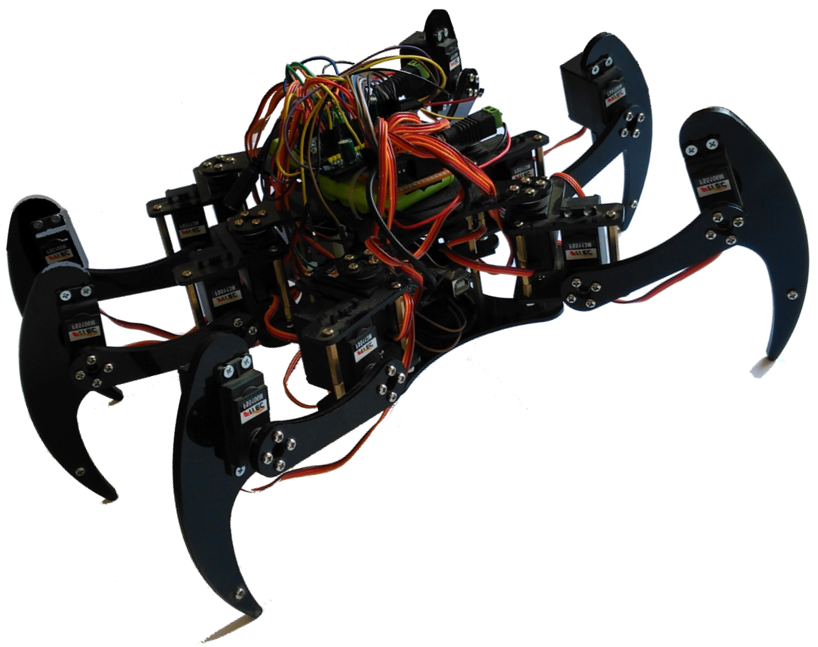
\includegraphics[width =0.8\textwidth]{Fig12}
    \caption{ A sex-legged walking robot.}
    \label{fig1}
\end{figure}

One of the interesting features of hexapod robots such as our ZagHexa (shown in Fig.\ref{fig1}) is that they can climb over obstacles larger than the equivalent sized wheeled or trucked vehicle. In fact, the use of wheels or crawlers limits the size of the obstacle that can be climbed to half the diameter of the wheels. On the contrary, legged robots can overcome obstacles that are comparable with the size of the machine leg\cite{2}. Hexapod walking robots also benefit from a lower impact on the terrain and have greater mobility in natural surroundings. This is especially important in dangerous environments like mine fields, or where it is essential to keep the terrain largely undisturbed for scientific reasons \cite{3}. \\

Hexapod legged robots have been used in exploration of remote locations and hostile environments such as seabed \cite{4}, in space or on planets \cite{5,6}  in nuclear power stations \cite{7}, and in search and rescue operations\cite{8}. Beyond this type of application, hexapod walking vehicles can also be used in a wide variety of tasks such as forests harvesting, in aid to humans in the transport of cargo, as service robots and entertainment. Development of hexapods is increasingly robust in the military sector. Armies all over the world are exploring ways of using hexapods to detect land mines, traverse rocky, unstable terrain, and carry out simple delivery missions in danger zones.

\section{History} 
Robots inspired by insects and other animals have previously been designed with physical antennae and tactile sensors to navigate their environment, as in the work by Brooks (1989) \cite{20,22}, Cowan et al. (2005), Hartmann (2001) \cite{27} and Lee et al. (2008) \cite{10}; the last three works employed the use of a single tactile element rather than a pair \cite{13}.
Because of their extreme mobility and agile adaptability to irregular terrain, insects have long been an inspiration for the designers of mobile and legged robots \cite{11,14}. Early hexapod robots such as Genghis and later creations such as Tarry implemented insect-like mobility based on observations of insect behaviors. The inter- leg coordination system developed by Holk Cruse \cite{30,23}  has been widely implemented   in legged hexapods and its basis is in behavioral experiments that qualitatively analyzed insect walking behaviors \cite{18}.

\subsection{Early Designs}
The first hexapods can be identified as robots based on a rigidly predetermined motion so that
an adaptation to the ground was not possible. Early researches in the 1950s were focused on assigning the motion control completely by a human operator manually\cite{11h}. 
\begin{figure}[h]
    \centering
    \begin{tabular}{ l l }
        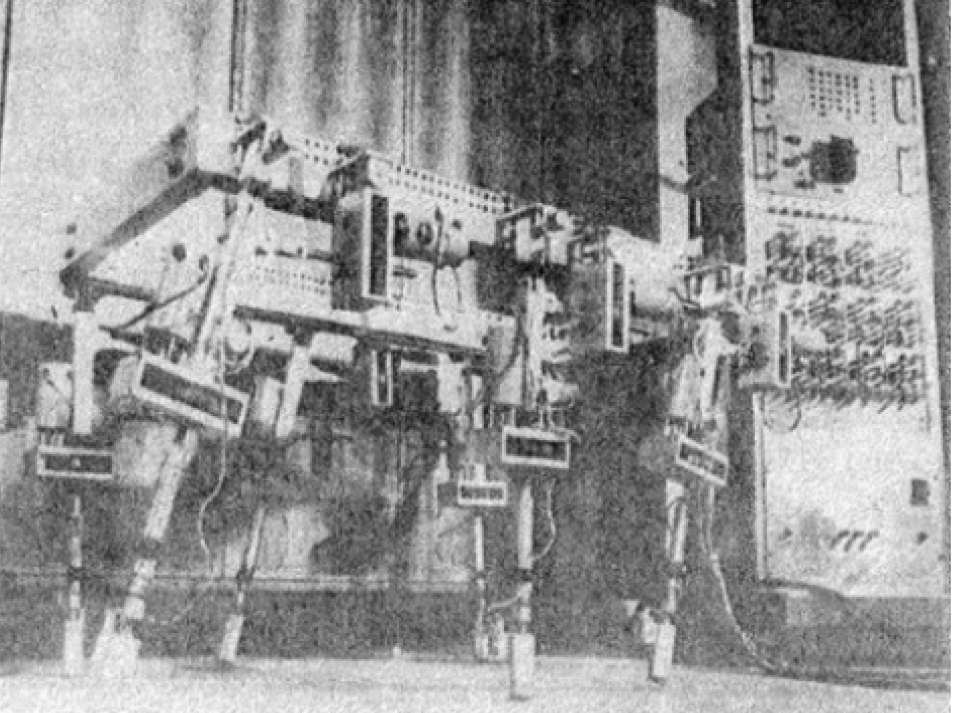
\includegraphics[width =.45\textwidth]{2_a} & 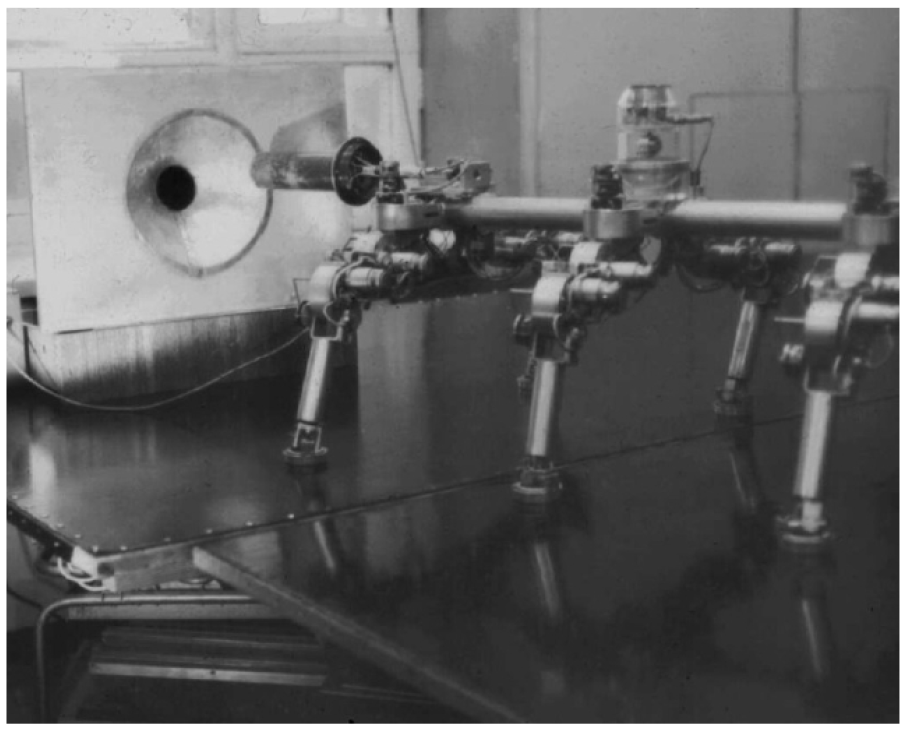
\includegraphics[width =.42\textwidth]{2_b} \\ 
        \hspace{3.5cm}(a) & \hspace{3.3cm}(b)\\
        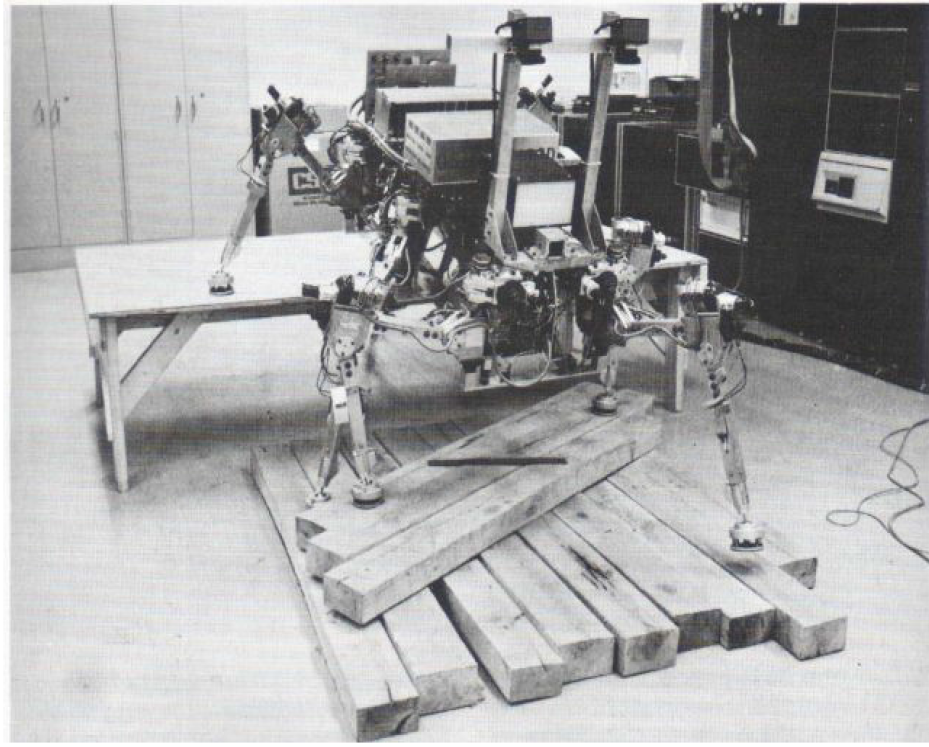
\includegraphics[width =.45\textwidth]{2_c} & \hspace{2cm} 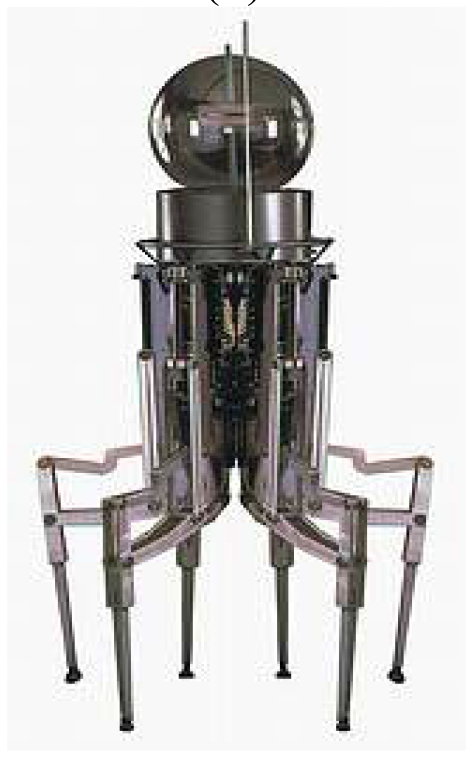
\includegraphics[width =.23\textwidth]{2_d} \\ 
        \hspace{3.5cm}(c) & \hspace{3.3cm}(d)\\
    \end{tabular}
    \caption{Early hexapod design: (a) University of Rome’s hexapod; (b) MASHA hexapod; (c) OSU hexapod; (d) ODEX I hexapod.}
    \label{fig2}
\end{figure}

One of the first successful hexapod robot was constructed at University of Rome in 1972 (Fig.\ref{fig2}a) as a computer-controlled walking machine with electric drives\cite{12h}. In the middle 70s, at the Russian Academy of Sciences in Moscow, a six-legged walking machine was developed with a mathematical model of motion control. It was equipped with a laser scanning range finder and was connected with a two-computer control system \cite{13h}. In 1976, Masha hexapod walking robot was designed at Moscow State University (Fig.\ref{fig2}b). The robot had a tubular axial chassis, articulated legs with three DoFs \cite{14h}. The hexapod was able to negotiate obstacles using contact on the feet and a proximity sensor. Ohio State University in 1977 developed a six-legged insect-like robot system called “OSU Hexapod” \cite{15h}. This hexapod was kept tethered and was made to walk short distances over obstacles (Fig.\ref{fig2}c).
In 1984, Odetic Inc., California, USA, developed Odex I \cite{17h}, a six-legged radially symmetric hexapod robot which used an onboard computer to play back pre-programmed motions (Fig.\ref{fig2}d).


\subsection{Recent Developments}
The two last decades have been characterized by a rapid development of control systems technology. Hexapod robots were equipped with various sensing systems. Artificial Intelligence systems were widely applied to the analysis of environment and motion of robots on a complex surface. A series of bio inspired robots was developed at Case Western Reserve University (USA) at the end the 90s, such as, for example, Robot III that had a total of 24 DoFs. Robot III architecture was based on the structure of cockroach, trying to imitate their behavior \cite{25h}. In particular, each rear leg had three DoFs, each middle leg four DoFs and each front leg five DoFs. Similarly, Biobot was a biomimetic robot physically modeled as the American cockroach (Periplaneta Americana) and powered by pressurized air \cite{26h}. This hexapod had a great speed and agility. \\
Each leg of the robot had three segments, corresponding to the three main segments of insect legs: coxa, femur, and tibia.
\begin{figure}[h]
    \centering
    \begin{tabular}{ l l }
        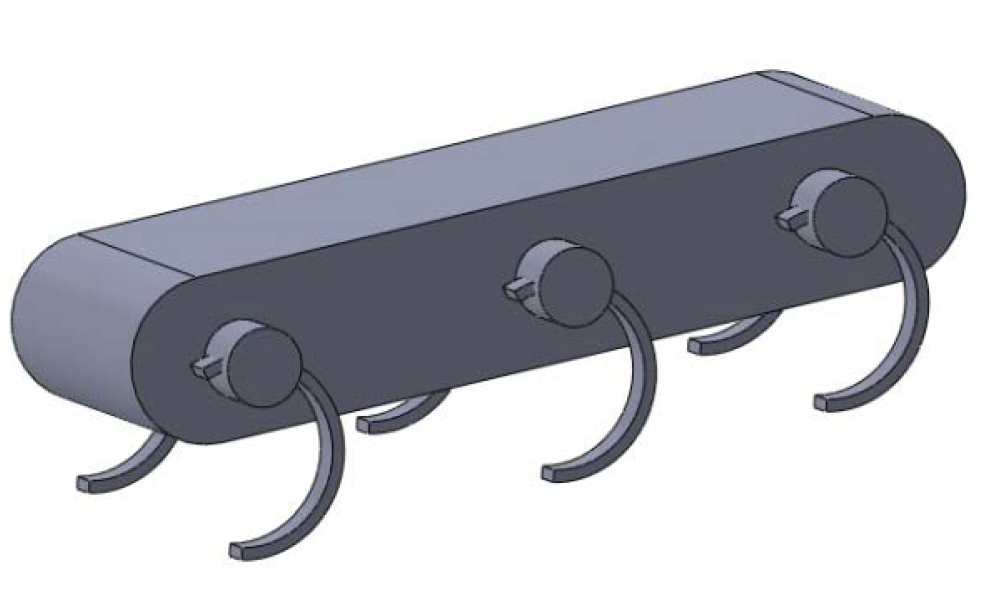
\includegraphics[width =0.45\textwidth,height=0.2\textheight]{3_a} & 
        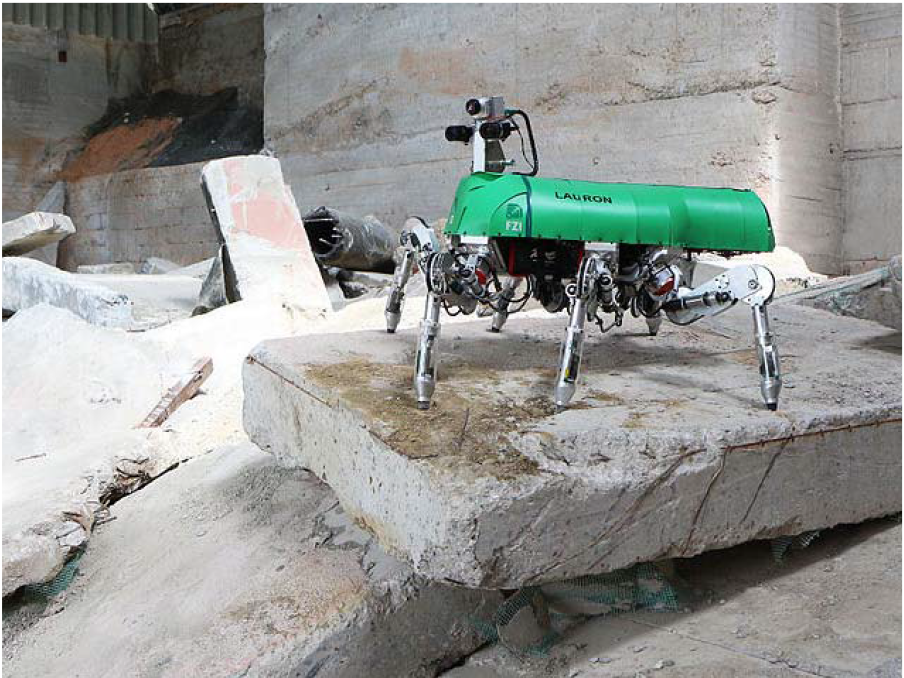
\includegraphics[width =0.45\textwidth,height=0.2\textheight]{3_b} \\ 
        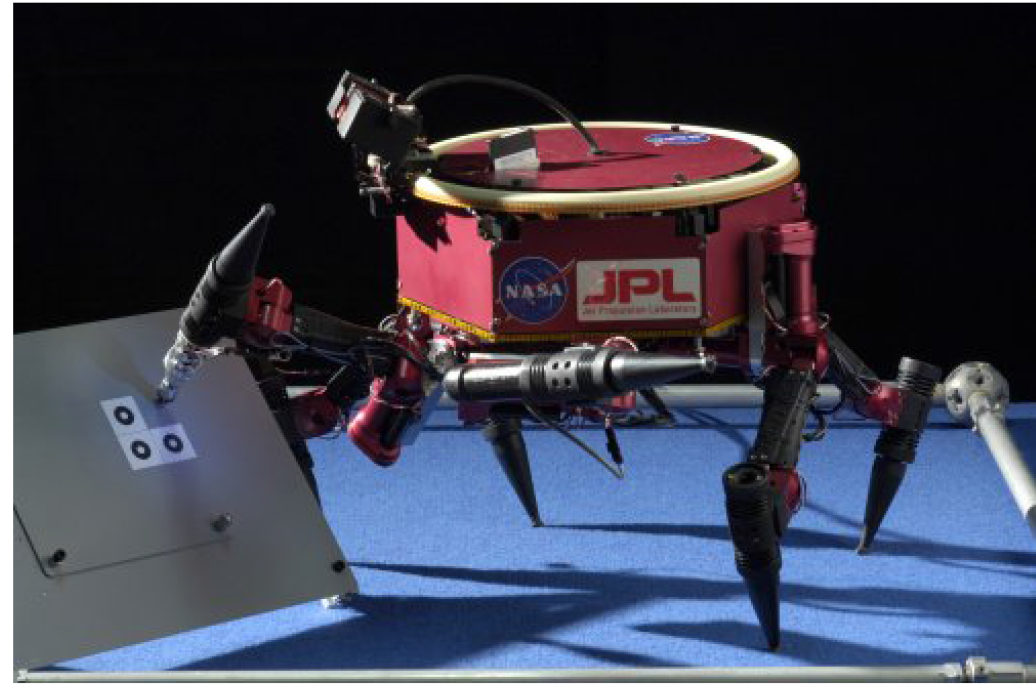
\includegraphics[width =0.45\textwidth,height=0.2\textheight]{3_c} & 
        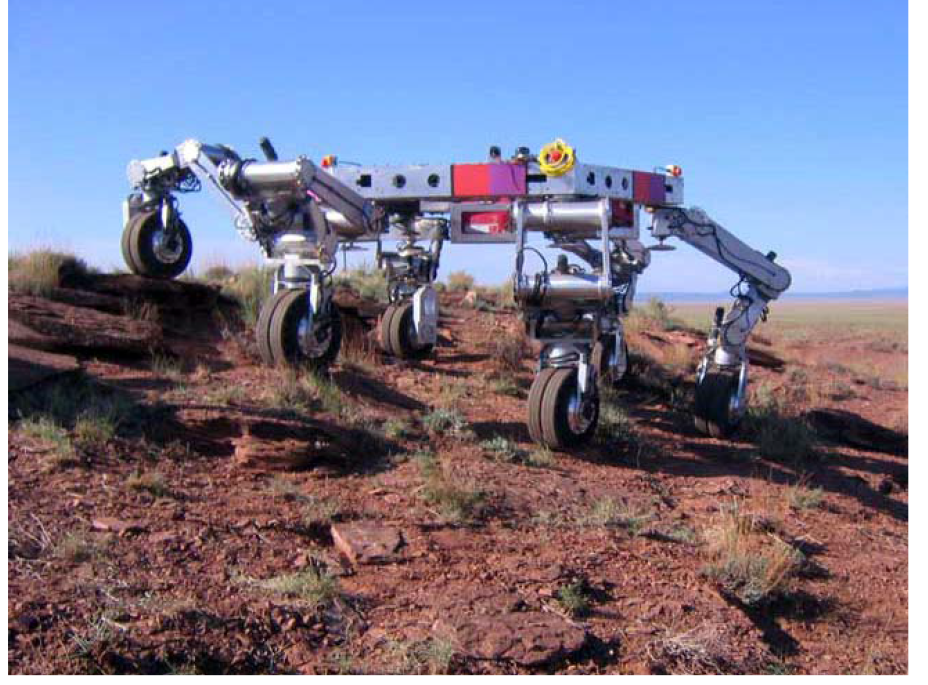
\includegraphics[width =0.45\textwidth,height=0.2\textheight]{3_d} \\ 
    \end{tabular}
    \caption{Some Example on recent developments in hexapod design}
    \label{fig3}
\end{figure}



%%%%%%%%%%%%%%%%%%%%%%%%%%%%%%%%%%%%%%%%%%%%%%%%%%%%%%%%%%%%%%%%%%%%%%%%%%%%%%%

\setchapterpreamble[o]{%
\dictum[Joseph Addison, \textit{(English essayist, poet, and politician, 1672--1719), Spectator, No. 253}]{% source: http://todayinsci.com/A/Addison_Joseph/AddisonJoseph-Quotations.htm
``It is impossible for us, who live in the latter ages of the world, to make observations in criticism, morality, or in any art or science, which have not been touched upon by others. We have little else left us but to represent the common sense of mankind in more strong, more beautiful, or more uncommon lights.''}\vspace{0.1em}}

\chapter{Hardware Design}\label{ch:design} %and Related Work
%Hardware design
In this chapter we will walk through the hardware design of our hexapod including both mechanical and electronic parts

\section{Design consideration}
Designing hexapod legged robots is far from trivial. A very numerous and a wide range of possibilities exist to design a hexapod. Designers must take several decisions which influence the operation and technical features. Some of the most important design issues and constraints according to \cite{48h} can be outlined as:

\begin{itemize}
	\item The mechanical structure of robot body.
	\item Leg architecture.
	\item Max sizes.
	\item Actuators and drive mechanisms.
	\item Control architecture.
	\item Power supply.
	\item Walking gaits and speed.
	\item Obstacle avoidance capability.
	\item Payload.
	\item Autonomy.
	\item Operation features.
	\item Cost.
\end{itemize}

The above mentioned design issues and constraints can be classified as design input (or key	features) and design output (or main design characteristics) as shown in the scheme of \ref{GD}.

\begin{figure}[H]		
	\centering
	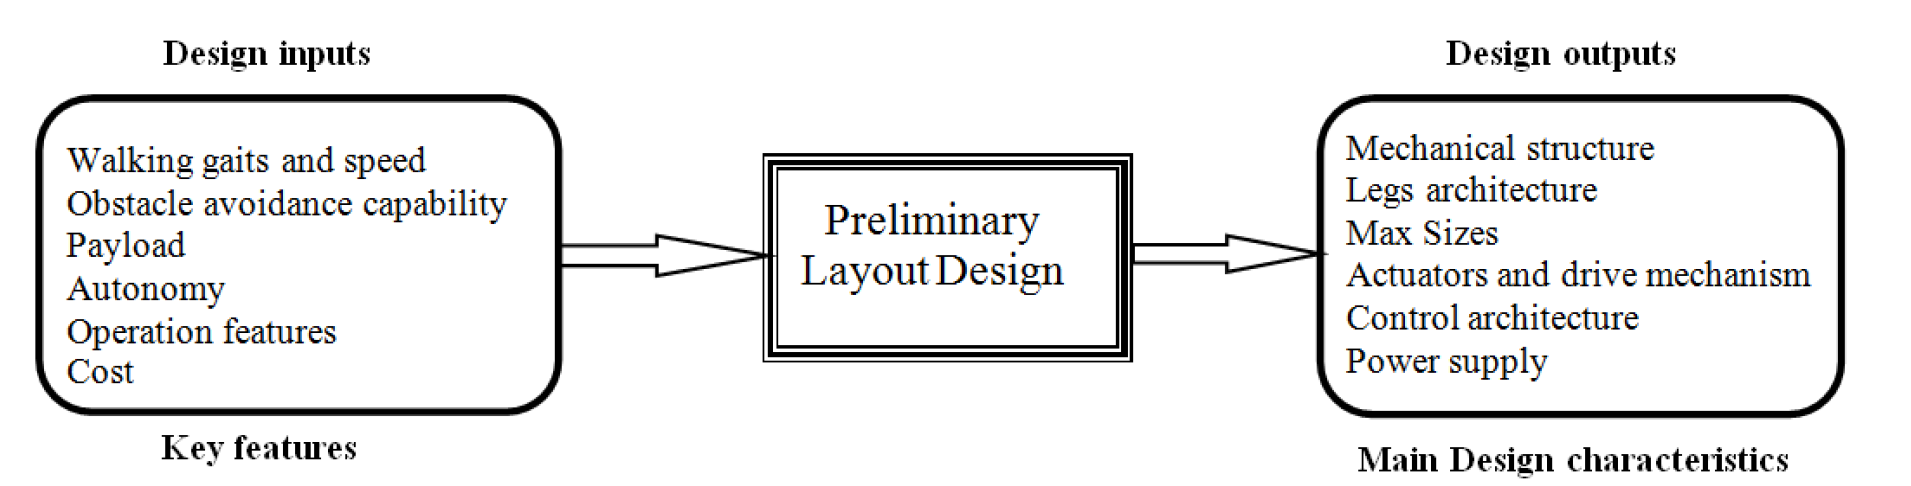
\includegraphics[width =.8\textwidth]{GD}
    \caption{ A scheme for preliminary layout design of hexapod walking robots.}
	\label{GD}
\end{figure}

\section{Hardware overview}
ZagHexa is a hexapod robot with 18 DOFs (three degrees of freedom (DOF) for each leg), it can walk in any direction (translation), or turn in place (rotation), or any combination of the two. The leg lift and ride height is adjustable as well. The robot uses a distributed walking control system based on the neurobiology of insects, stepping in the sagittal plane to angled stepping, which then induces turning in the robot.
It is an integrated multi-legged walking robot based on de-facto standard Robotic Operating System (ROS) that employs novel and different walking patterns.
Our robot is teleoperated using hand-held devices such as a smart phone or tablet or a wireless joystick (see Fig.\ref{fig4}). Furthermore, it has its own navigation system and a camera for instant video recording and streaming.
The power to the entire system is supplied through two 5 volts NiMH batteries. There is an additional power bank to power up the Raspberry Pi and other electronic components. 

\begin{figure}[H]
	\centering
	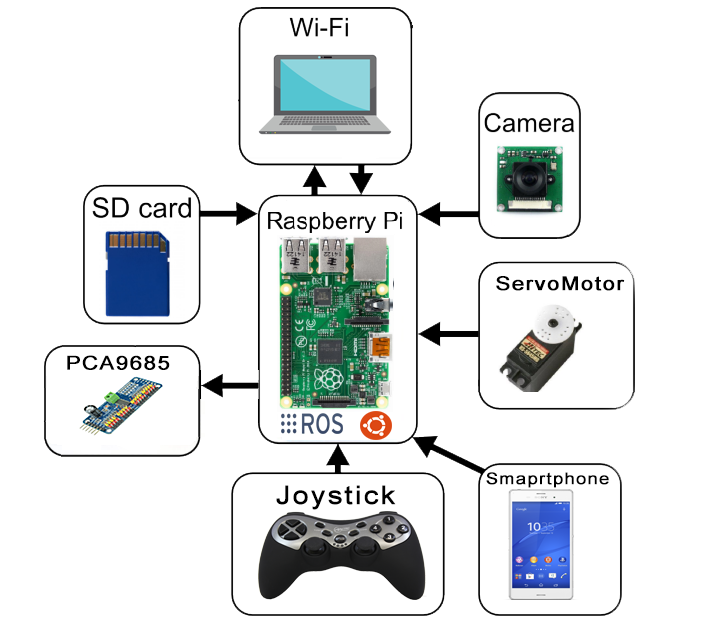
\includegraphics[width =.5\textwidth]{Fig2}
	\caption{ The electronic system of the robot.}
	\label{fig4}
\end{figure}

The final design of the ZagHexa robot constructed mainly with acrylic is shown in Fig.\ref{fig1}. ZagHexa body moves independently of its ground contact points. To make its center of gravity shift on a horizontal plane, forward/backward, and sideways moving functions are effective. These functions can also produce a smooth body movement independently of intermittent leg traveling. The robot has been designed with three degrees of freedom in the front, middle and rear legs respectively. The physical specifications are given in Table 2.
\begin{center}
\begin{tabular}{|c|c|}
    \hline
    Parameter       &       Description        \\ \hline
    Length         &           30cm           \\ \hline
    Width         &           27cm           \\ \hline
    Height         &           17cm           \\ \hline
    Weight         &           3Kg            \\ \hline
    Construction Material &                          \\ \hline
    Actuators       &     DC servo motors      \\ \hline
    Motion Control     & Servo Sequential Control \\ \hline
    Leg Stroke (Max)    &           6cm            \\ \hline
    Leg Lift (Max)     &           5cm            \\ \hline
\end{tabular}
\end{center}
\noindent
%Mechanical design
\section{Mechanical design}
\noindent In this section we will discuss the different designs of the robot including early ones as well as the final one.
\subsection{Micro ZagHexa}
We started by making a small hexapod with 18 micro servos to test our basic functions and walking algorithms. The basic parts of Micro ZagHexa is made of a 1 mm thick Aluminium sheet.

\begin{figure}[H]
	\centering
	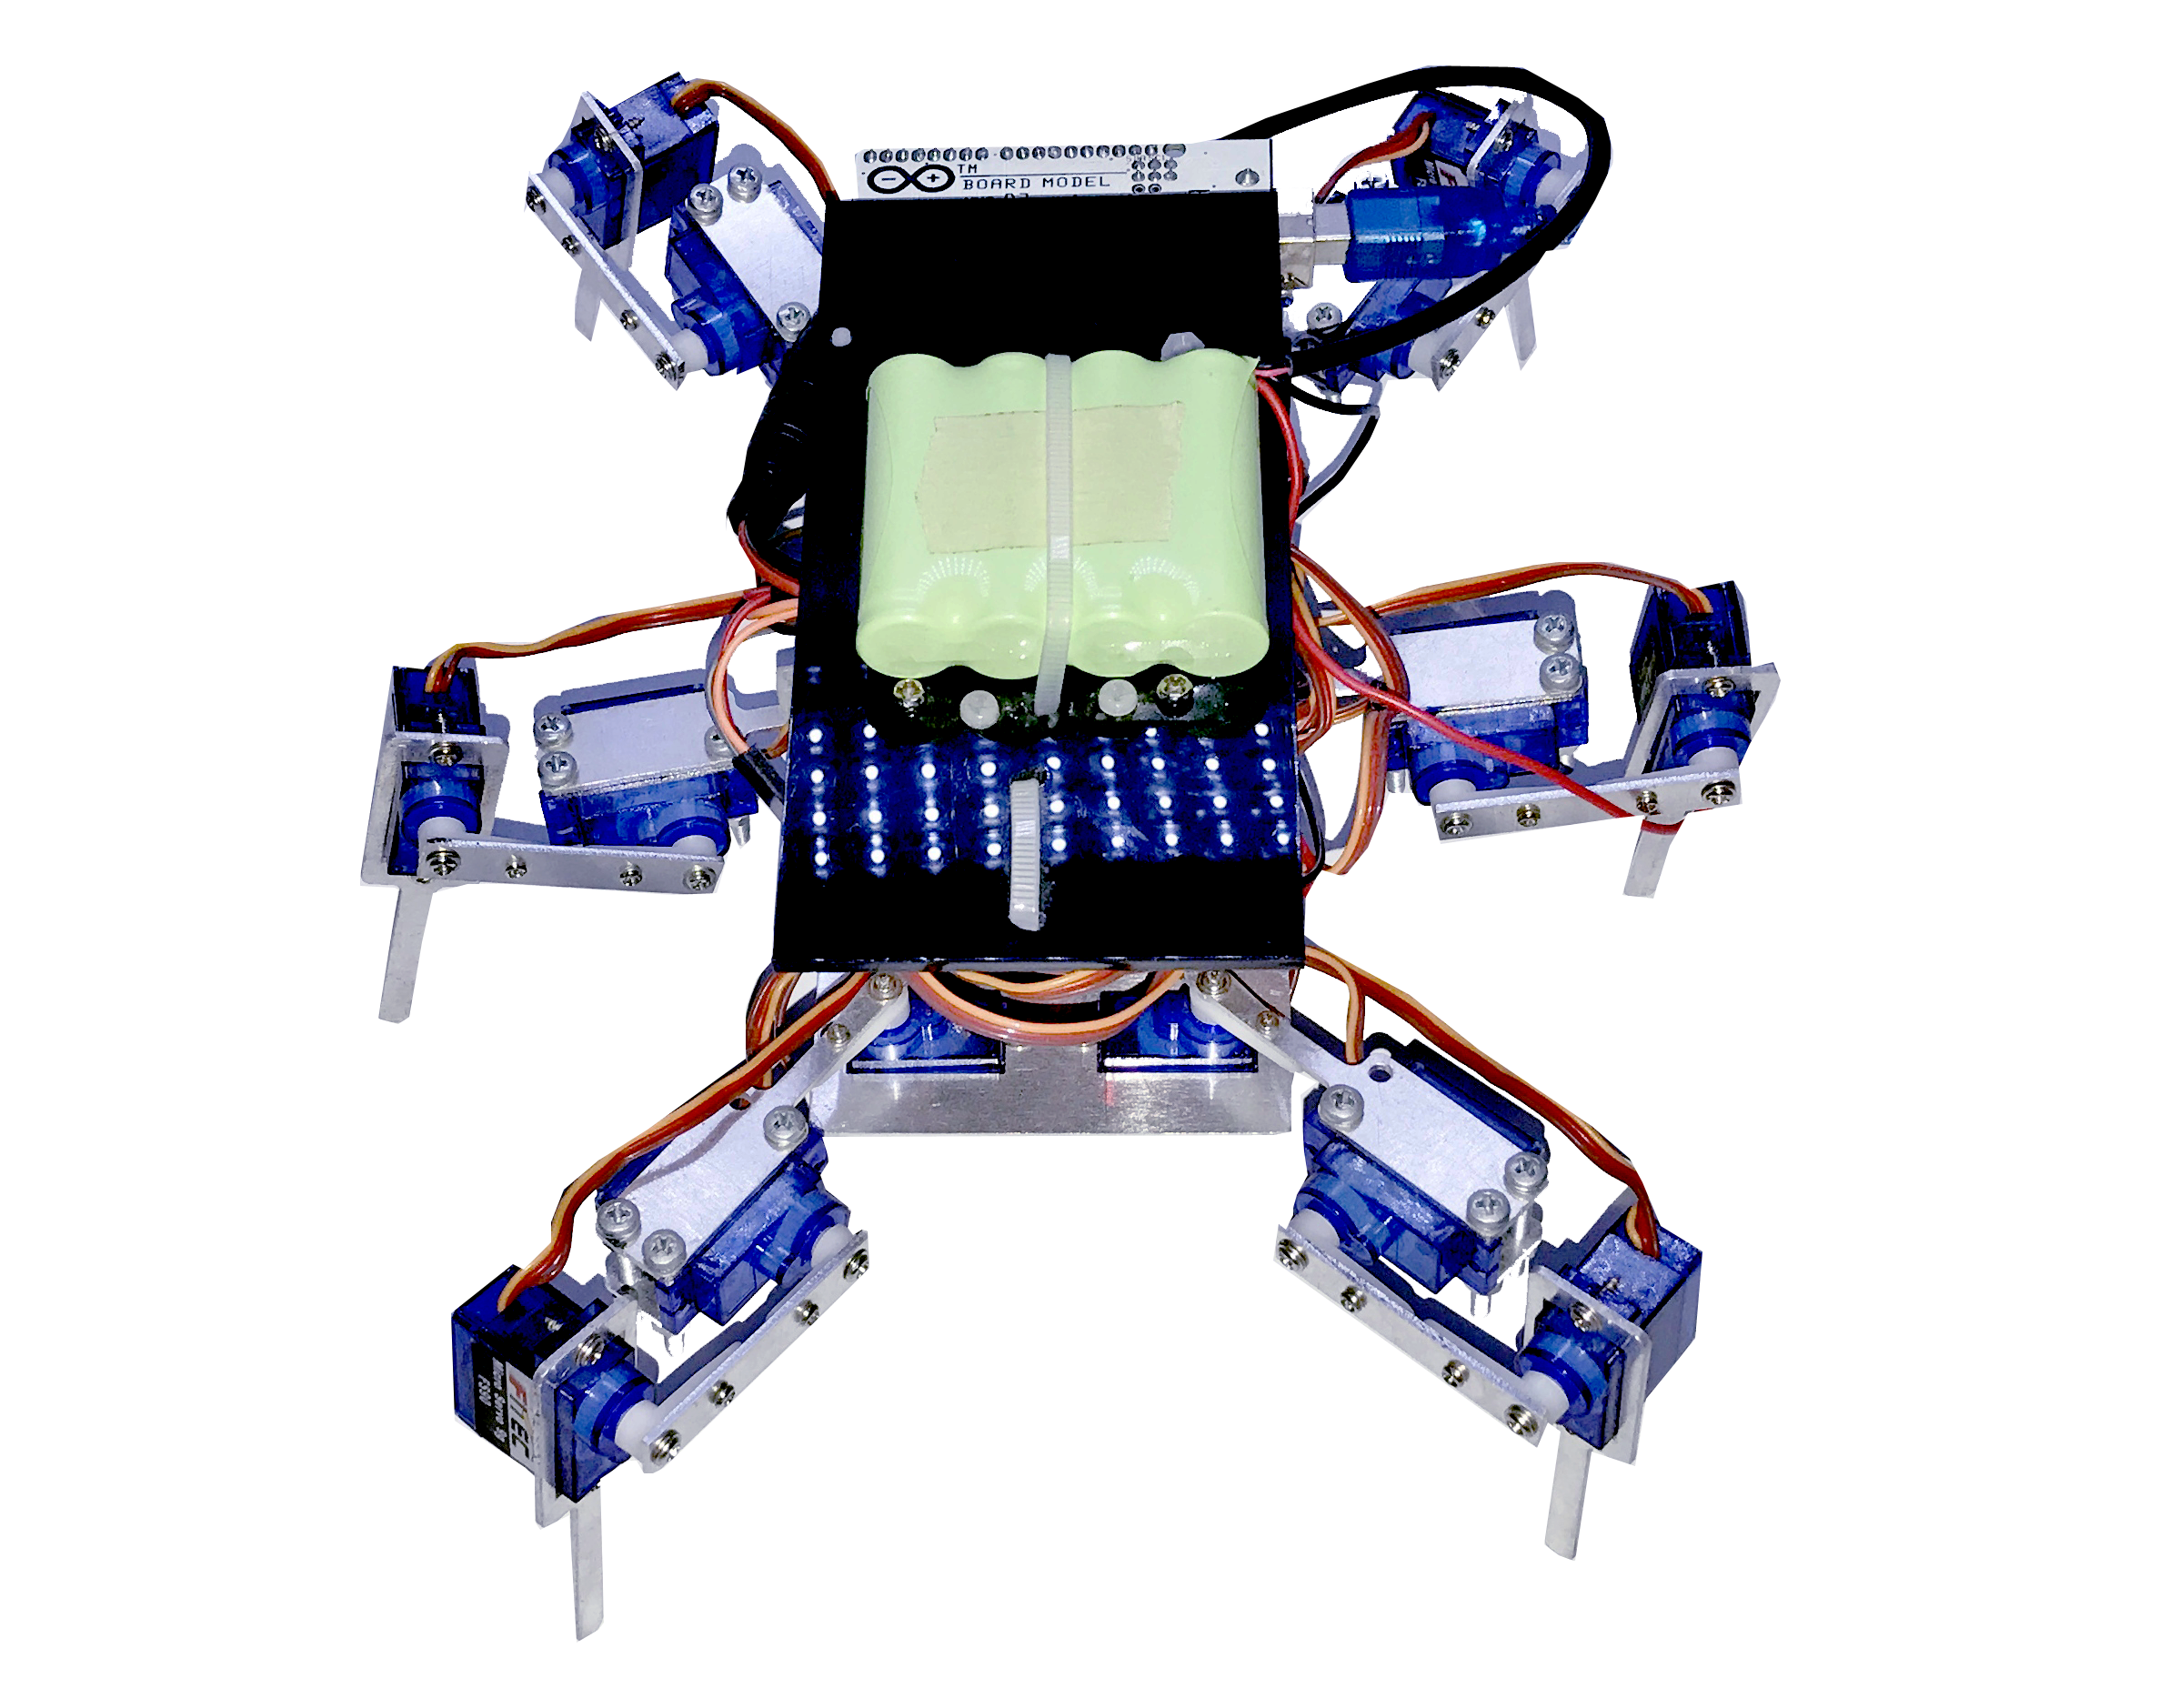
\includegraphics[width=5cm,height=5cm]{figures/uZagHexaFinal.png}
	\caption{Micro ZagHexa}
	\label{figure_i}
\end{figure}

\subsection{ZagHexa}
We moved to our next hexapod design and made it bigger and more natural looking with an articulate leg and body design. ZagHexa is made of 2.5 mm thick Acrylic. \ref{figure_} shows the CAD model of Zaghexa and \ref{figure_} shows it after being assembled.
%\begin{figure}[h]
%	\centering
%	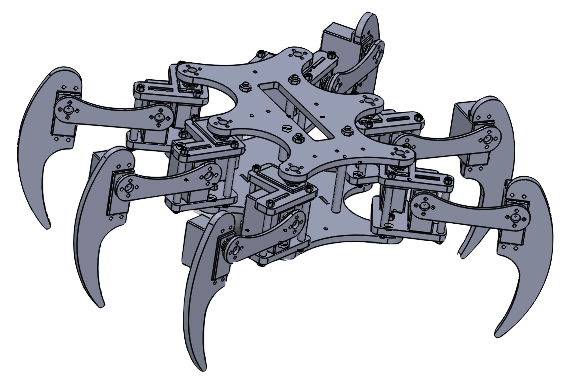
\includegraphics{figure_j}
%	\caption{CAD model of ZagHexa}
%	\label{figure_j}
%\end{figure}
\begin{figure}[H]
	\centering
	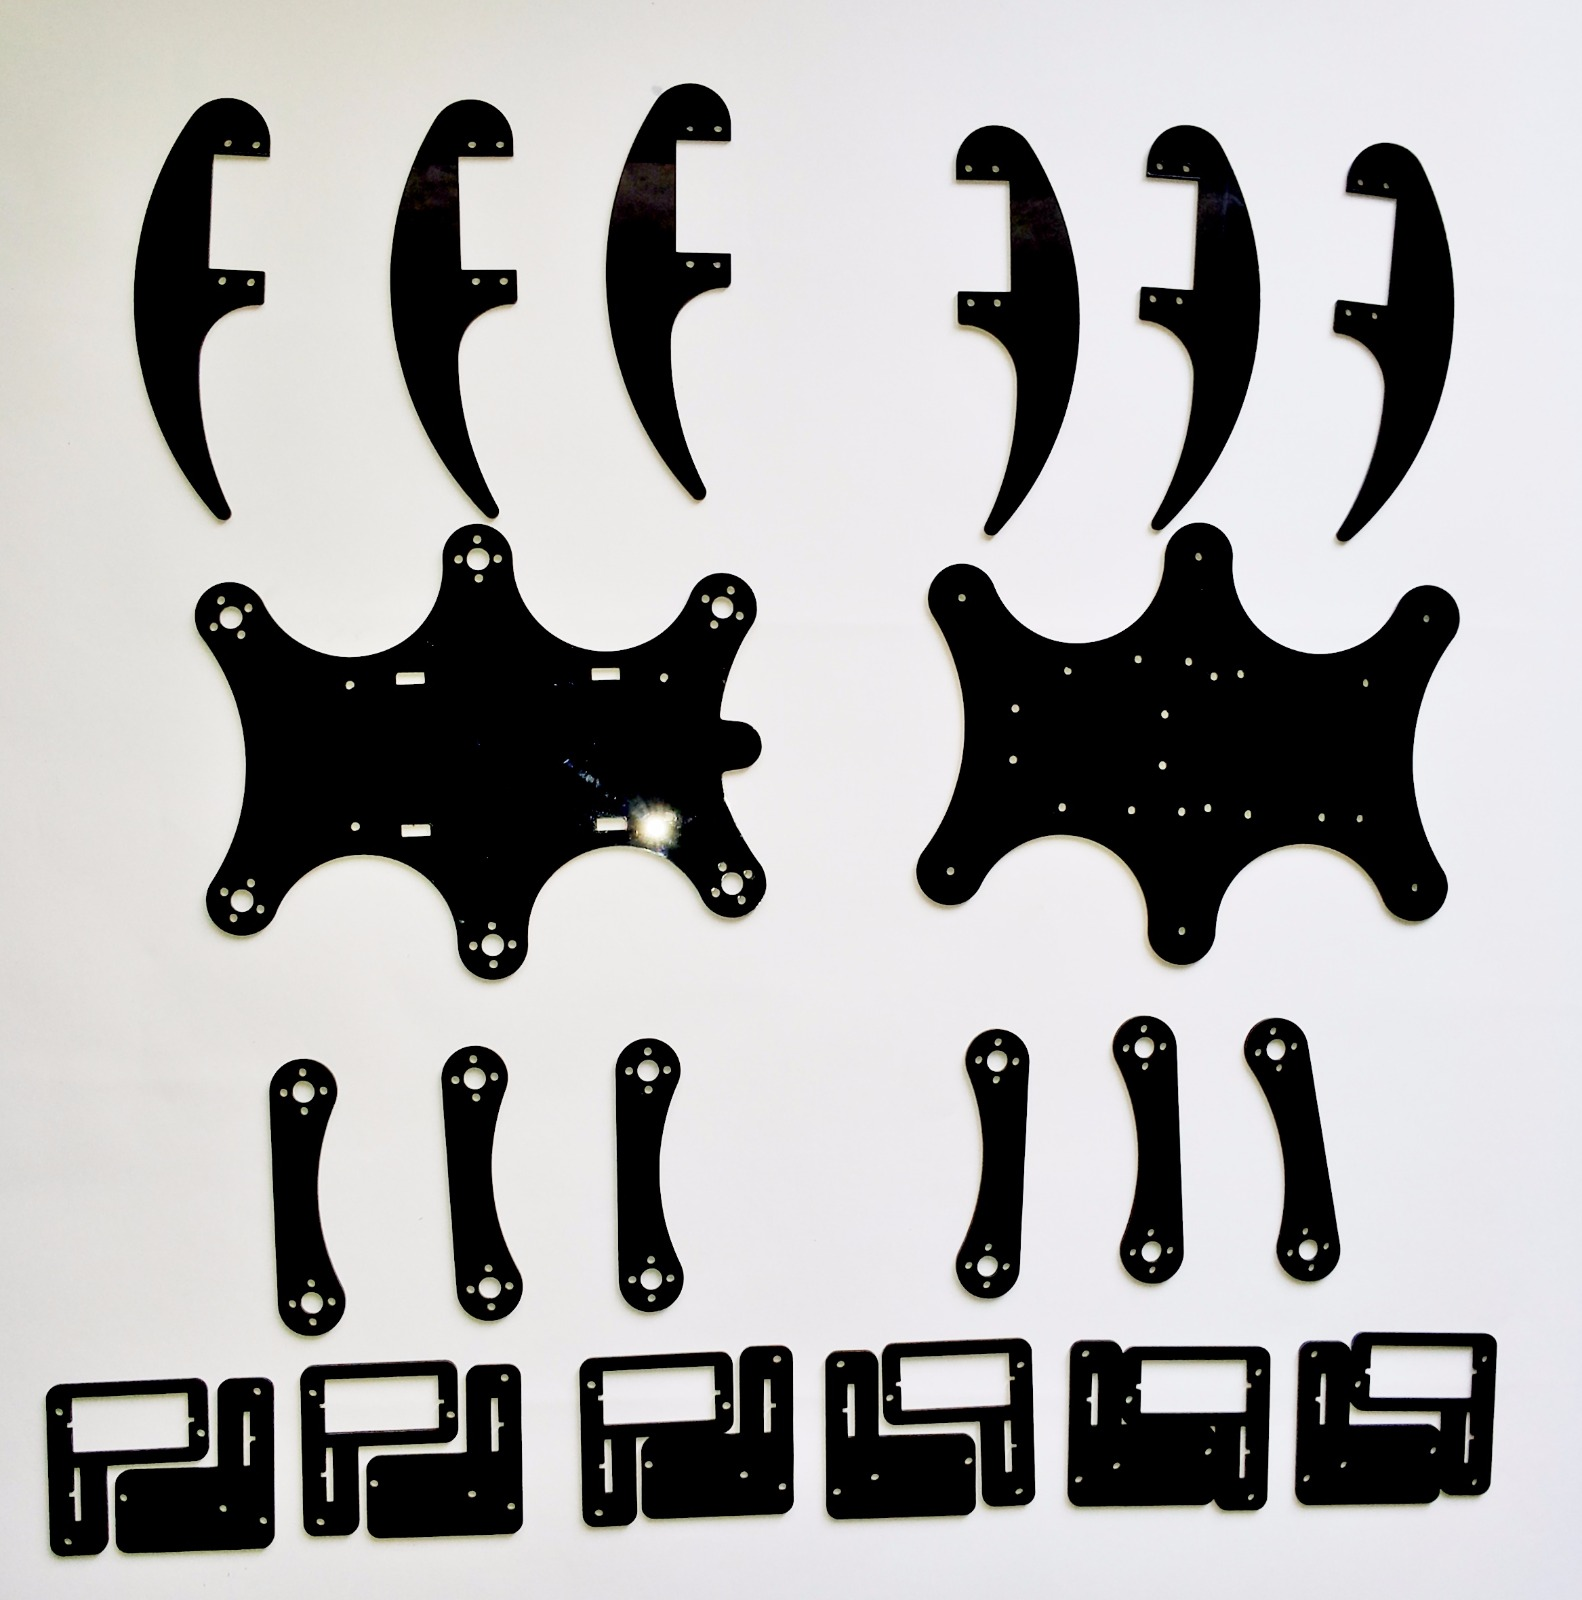
\includegraphics[width=10cm,height=11cm]{figure_k}
	\caption{ZagHexa during assembling}
	\label{figure_k}
\end{figure}
\begin{figure}[H]
	\centering
   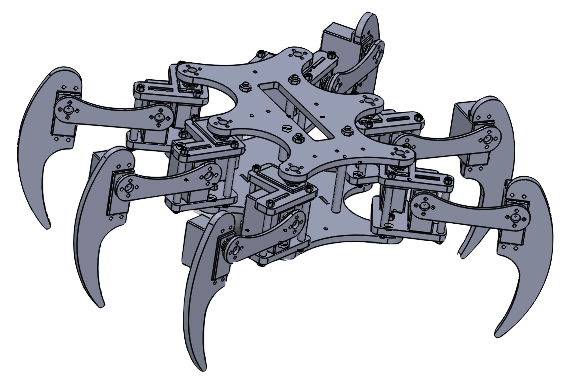
\includegraphics[width=0.45\textwidth]{figure_j}
	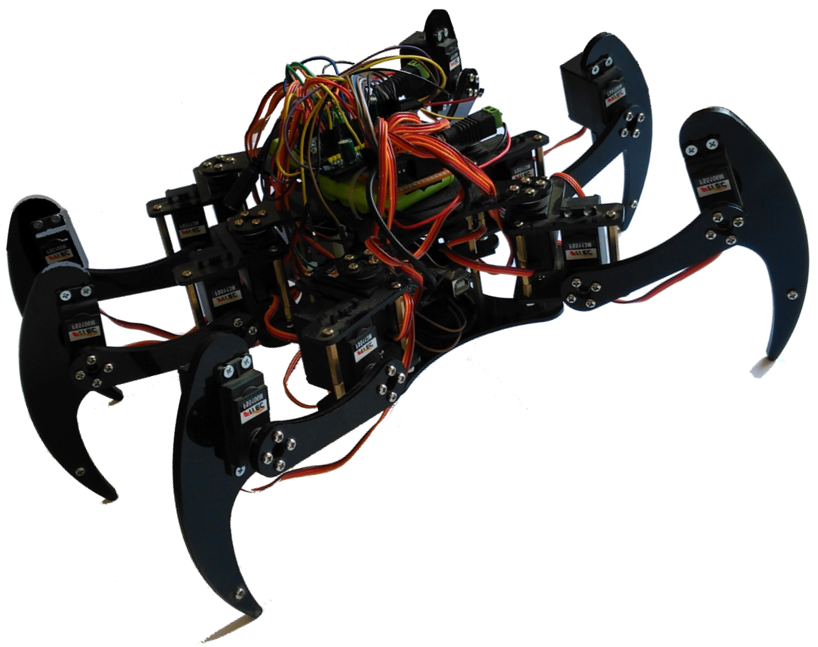
\includegraphics[width=0.45\textwidth]{Fig12}
	\caption{CAD model (left) and assembled ZagHexa (right)}
	\label{figure_l}
\end{figure}

\subsection{Giant ZagHexa}
Lastly, we made the giant version of our hexapod. It is made of a double layer 1 mm thick Aluminium sheet. The CAD model of Giant ZagHexa is shown in \ref{figure_m} and \ref{figure_o} shows it after assembling.
\begin{figure}[H]
	\centering
	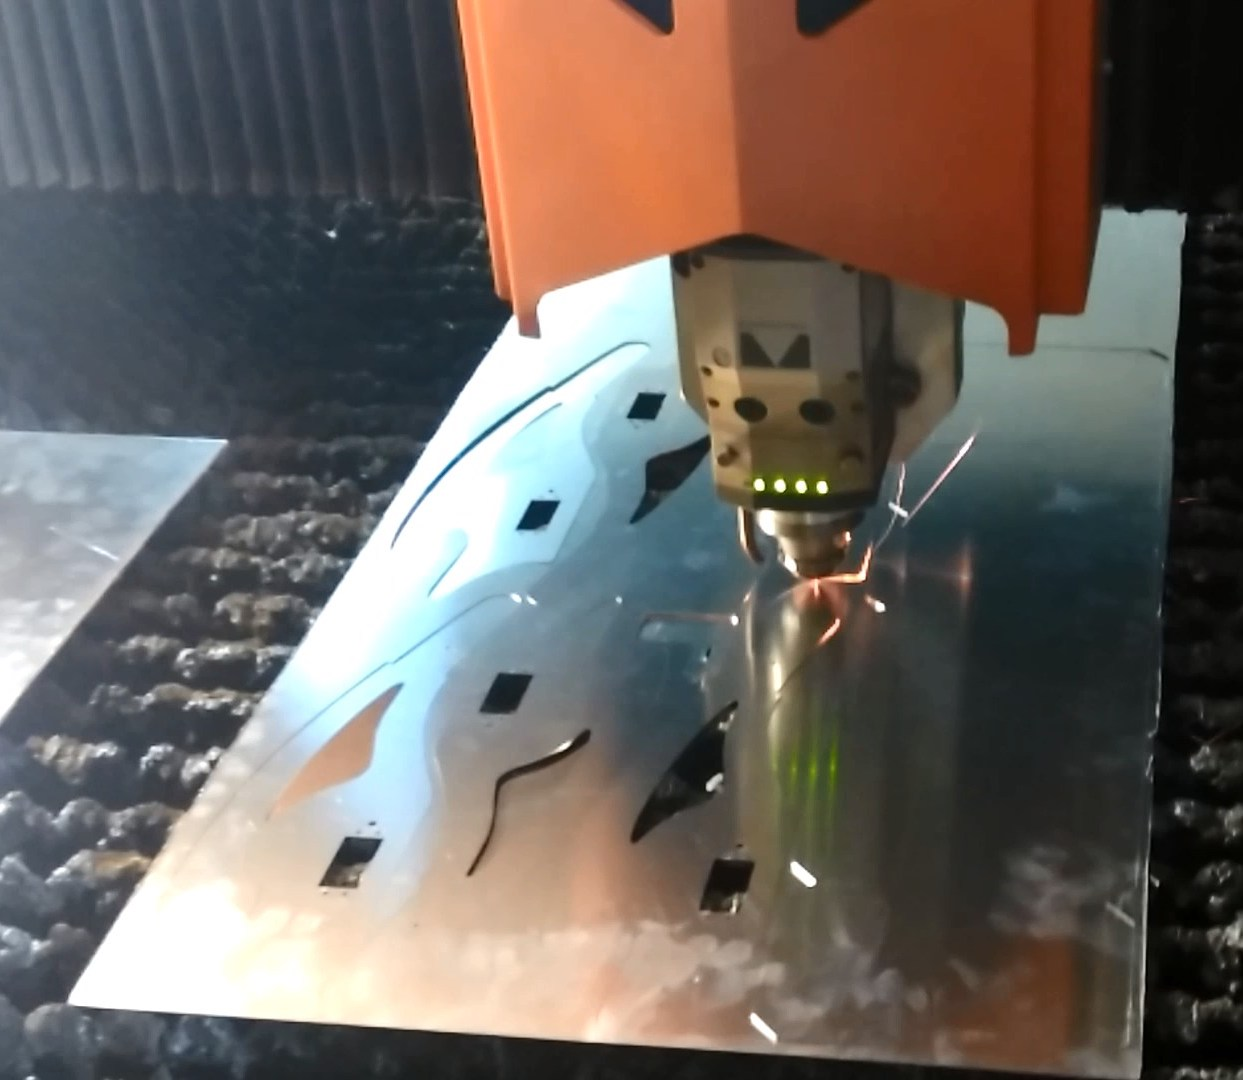
\includegraphics[width=0.7\textwidth]{figure_n}
	\caption{Giant ZagHexa during laser cutting}
	\label{figure_n}
\end{figure}
\begin{figure}[H]
	\centering
    	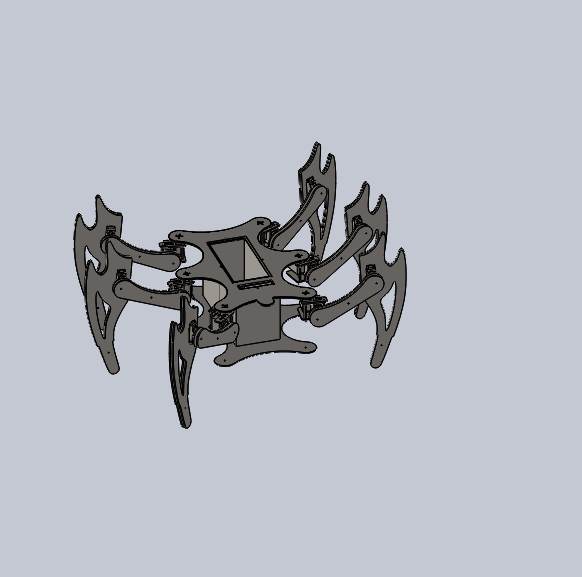
\includegraphics[width=0.45\textwidth]{figure_m}
	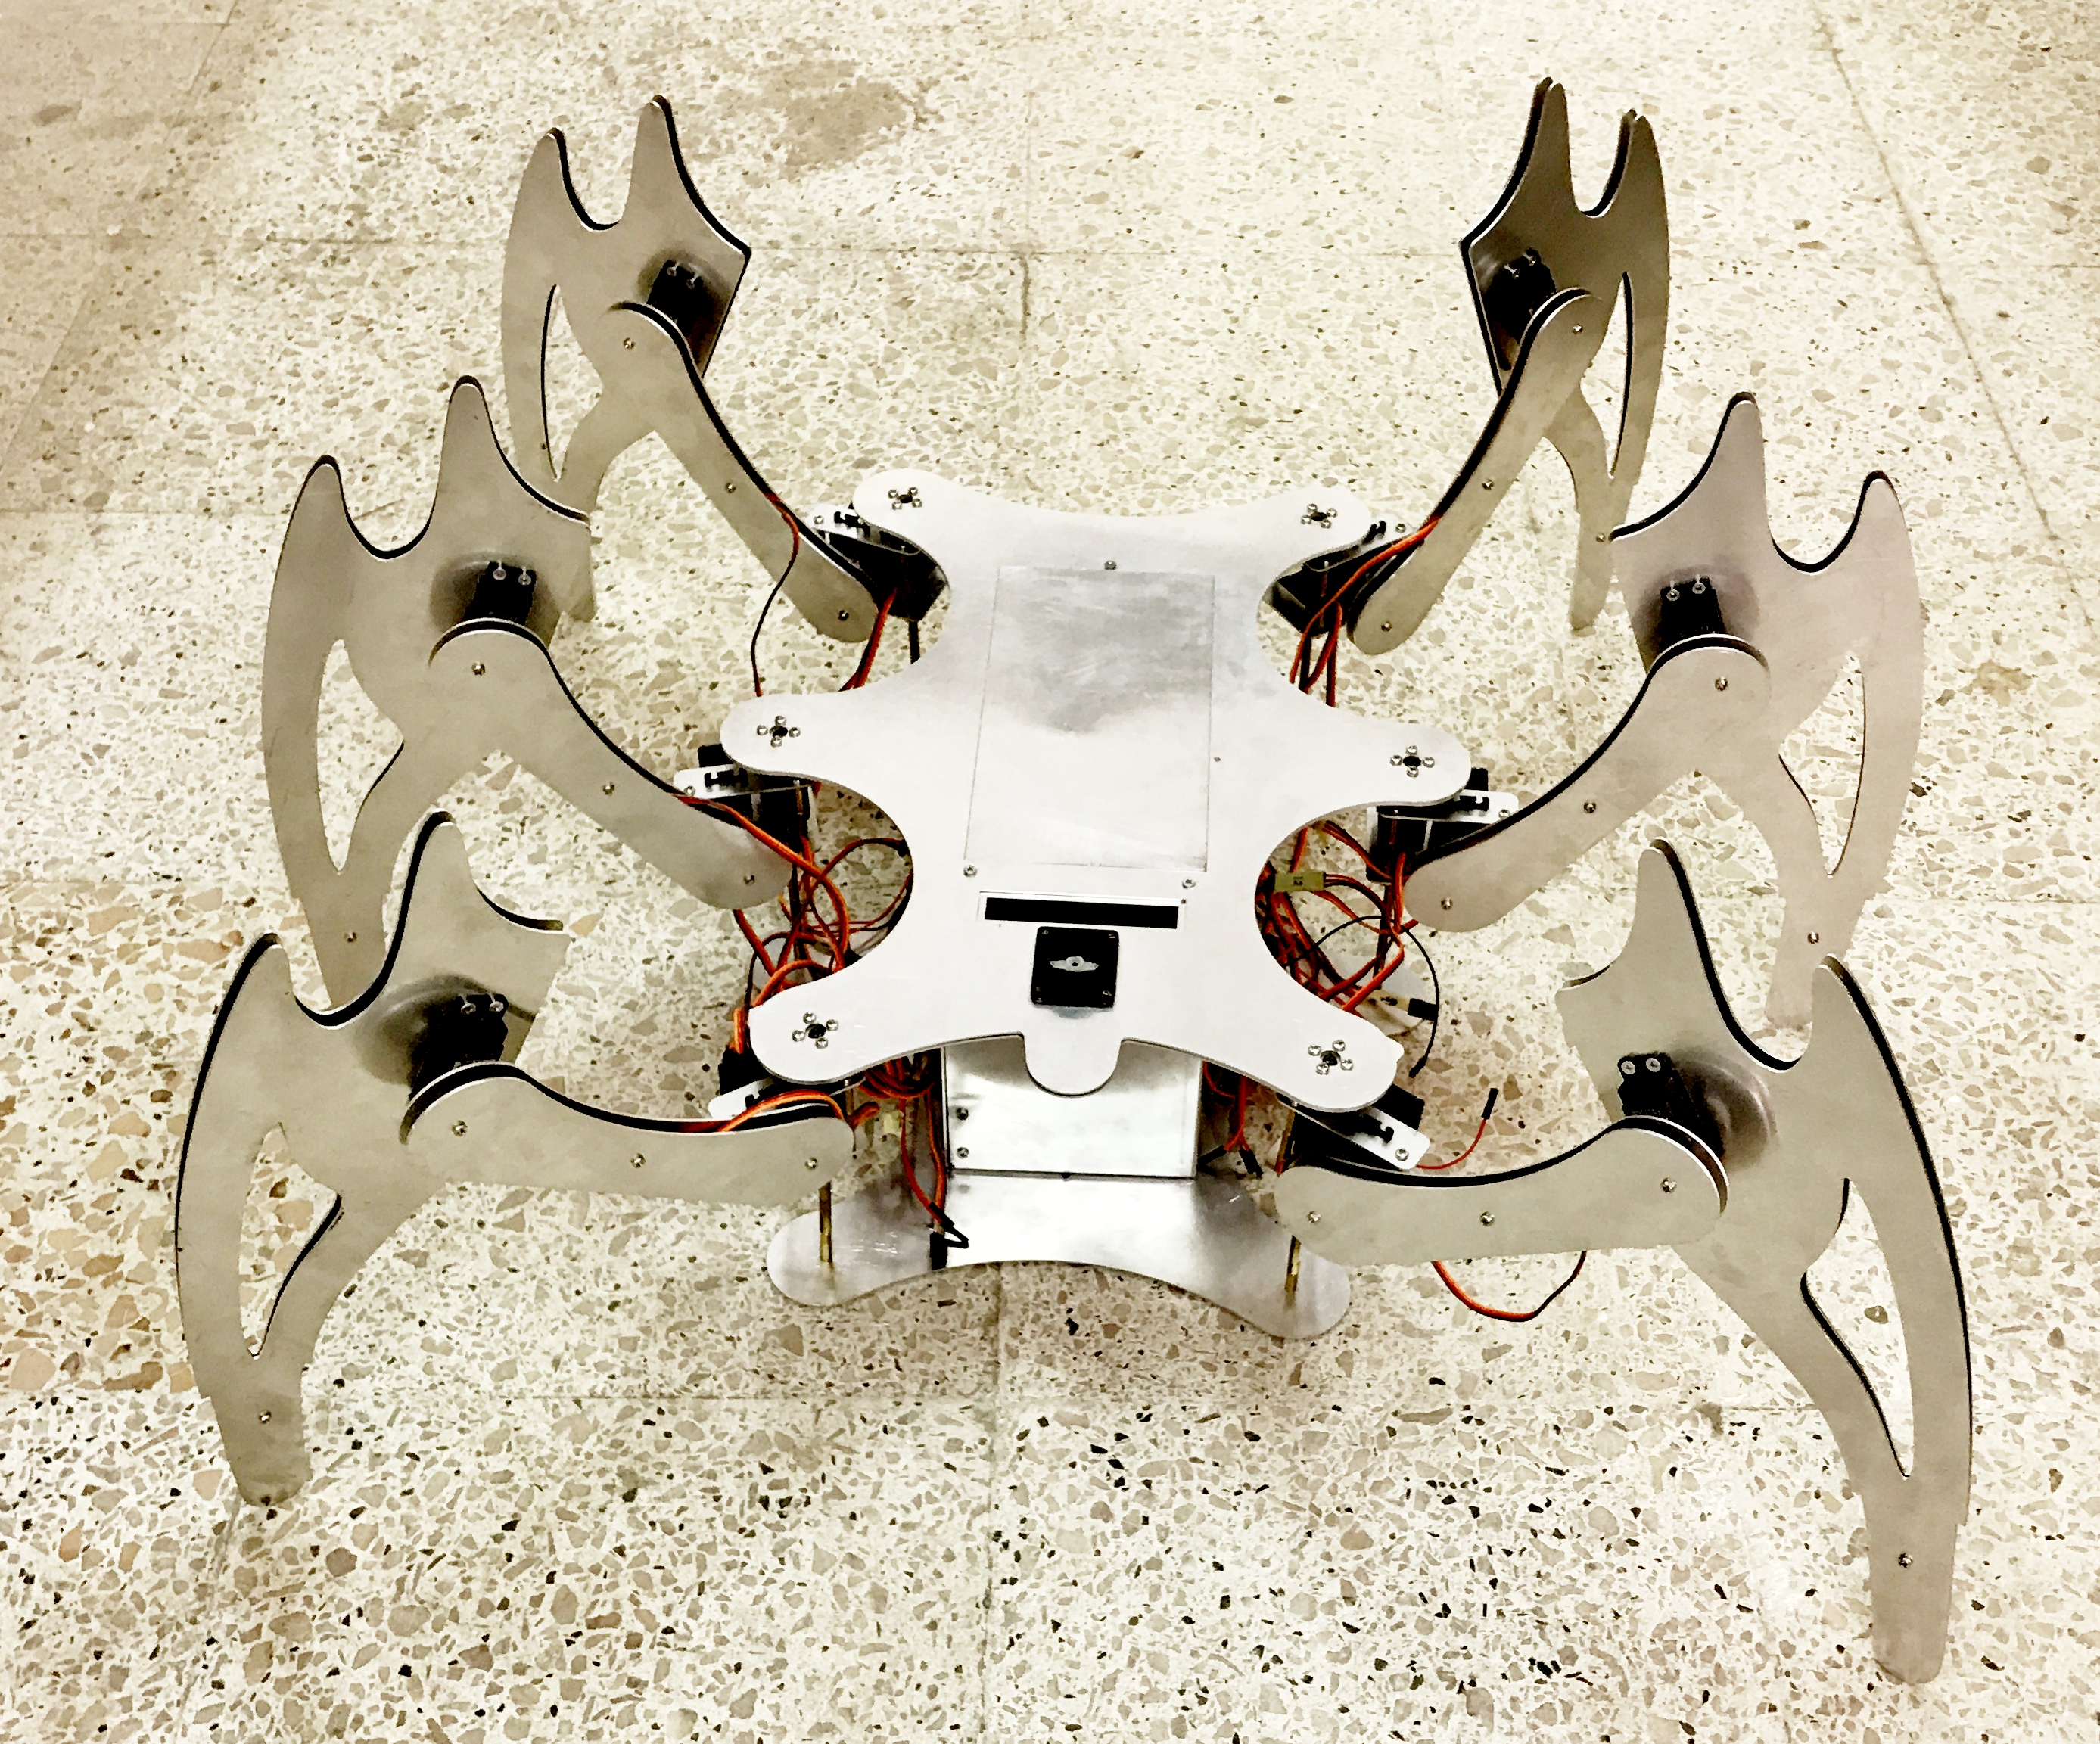
\includegraphics[width=0.45\textwidth]{figure_o}
	\caption{CAD model (left) and assembled Giant ZagHexa (right)}
	\label{figure_o}
\end{figure}


The giant ZagHexa was a little disappointing as servo motors were not strong enough to drive our hexapod. We tried to make the chassis lighter but that did not solve the problem completely. It still have stability issues.

%Electronics
\section{Electronics}
In this section we will talk about the electronic components we have been using through the whole project.
\subsection{Adafruit PCA9685}
Firstly, we used the Adafruit PCA9685 servo controller shown in \ref{figure_i} and \ref{figure_j}. Although driving servo motors with the Arduino Servo library is pretty easy, each one consumes a precious pin - not to mention some Arduino processing power.  The Adafruit 16-Channel 12-bit PWM/Servo Driver will drive up to 16 servos over I2C with only 2 pins.  The on-board PWM controller will drive all 16 channels simultaneously with no additional Arduino processing overhead.  Moreover, we can chain up to 62 of them to control up to 992 servos - all with the same 2 pins!
\begin{figure}[H]
	\centering
	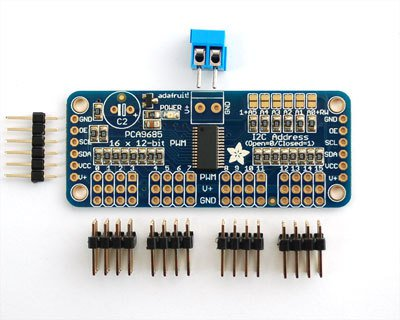
\includegraphics{figure_i}
	\caption{Adafruit PCA9685}
	\label{figure_i}
\end{figure}
\begin{figure}[H]
	\centering
	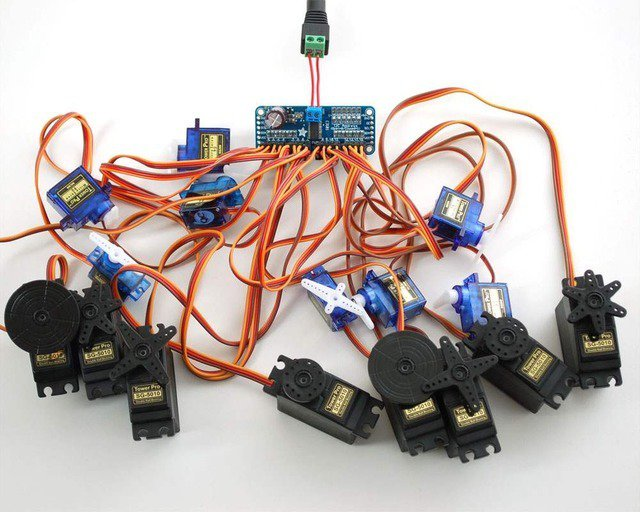
\includegraphics[width=14cm,height=10cm]{figure_p}
	\caption{Adafruit PCA9685 wiring}
	\label{figure_p}
\end{figure}
\subsection{Servo Motors}
We used 18 servo motors of different sizes as actuators. A 7 kg.cm servo motor is used to drive the tibia part as well as the coxa. The motor that will lift the whole leg should be much stronger so we used a 13 kg.cm servo. That's it, we have 3 servo motors in each leg(3 DOFs): one for coxa and one for tibia and a stronger one for the femur.

\begin{figure}[H]
	\centering
	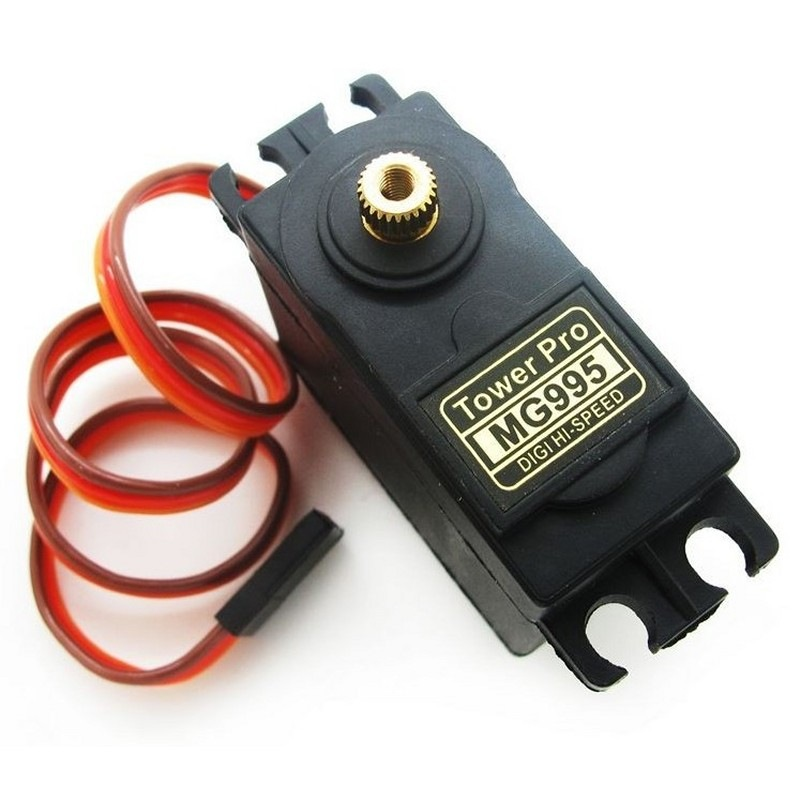
\includegraphics[width=10cm,height=5cm]{figure_q}
	\caption{13 kg.cm servo motor}
	\label{figure_q}
\end{figure}

\subsection{Playstaion joystick}
In earlier versions of ZagHexa, we used a wireless playstation 2 controller to teleoperate the hexapod. It communicates with the arduino through its uniqe via an SPI communication protocol.

\begin{figure}[H]
	\centering
	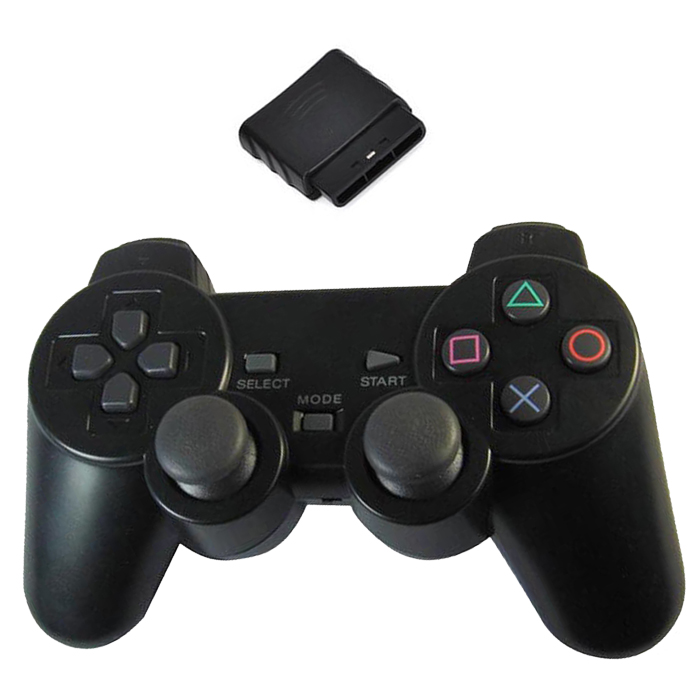
\includegraphics{figure_r}
	\caption{Playstaion 2 controller}
	\label{figure_r}
\end{figure}

\subsection{PS2/Serial converter}
A converter is used to keep the communication between the joystick and the controller happens serially so it well be easier to handle.

\begin{figure}[H]
	\centering
	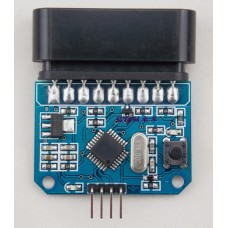
\includegraphics[width=6cm,height=8cm]{figure_s}
	\caption{PS2/Serial adapter}
	\label{figure_s}
\end{figure}

\subsection{Arduion Mega}
Later, we use an Arduino Mega in replacement of the PCA 9685 servo controller to send PWM signals to each servo motor. The reason why we moved our work from the servo controller to the Arduino Mega is that the servo controller can NOT withstand voltage above 6 Volts nor current above 5 Amps.

\begin{figure}[H]
	\centering
	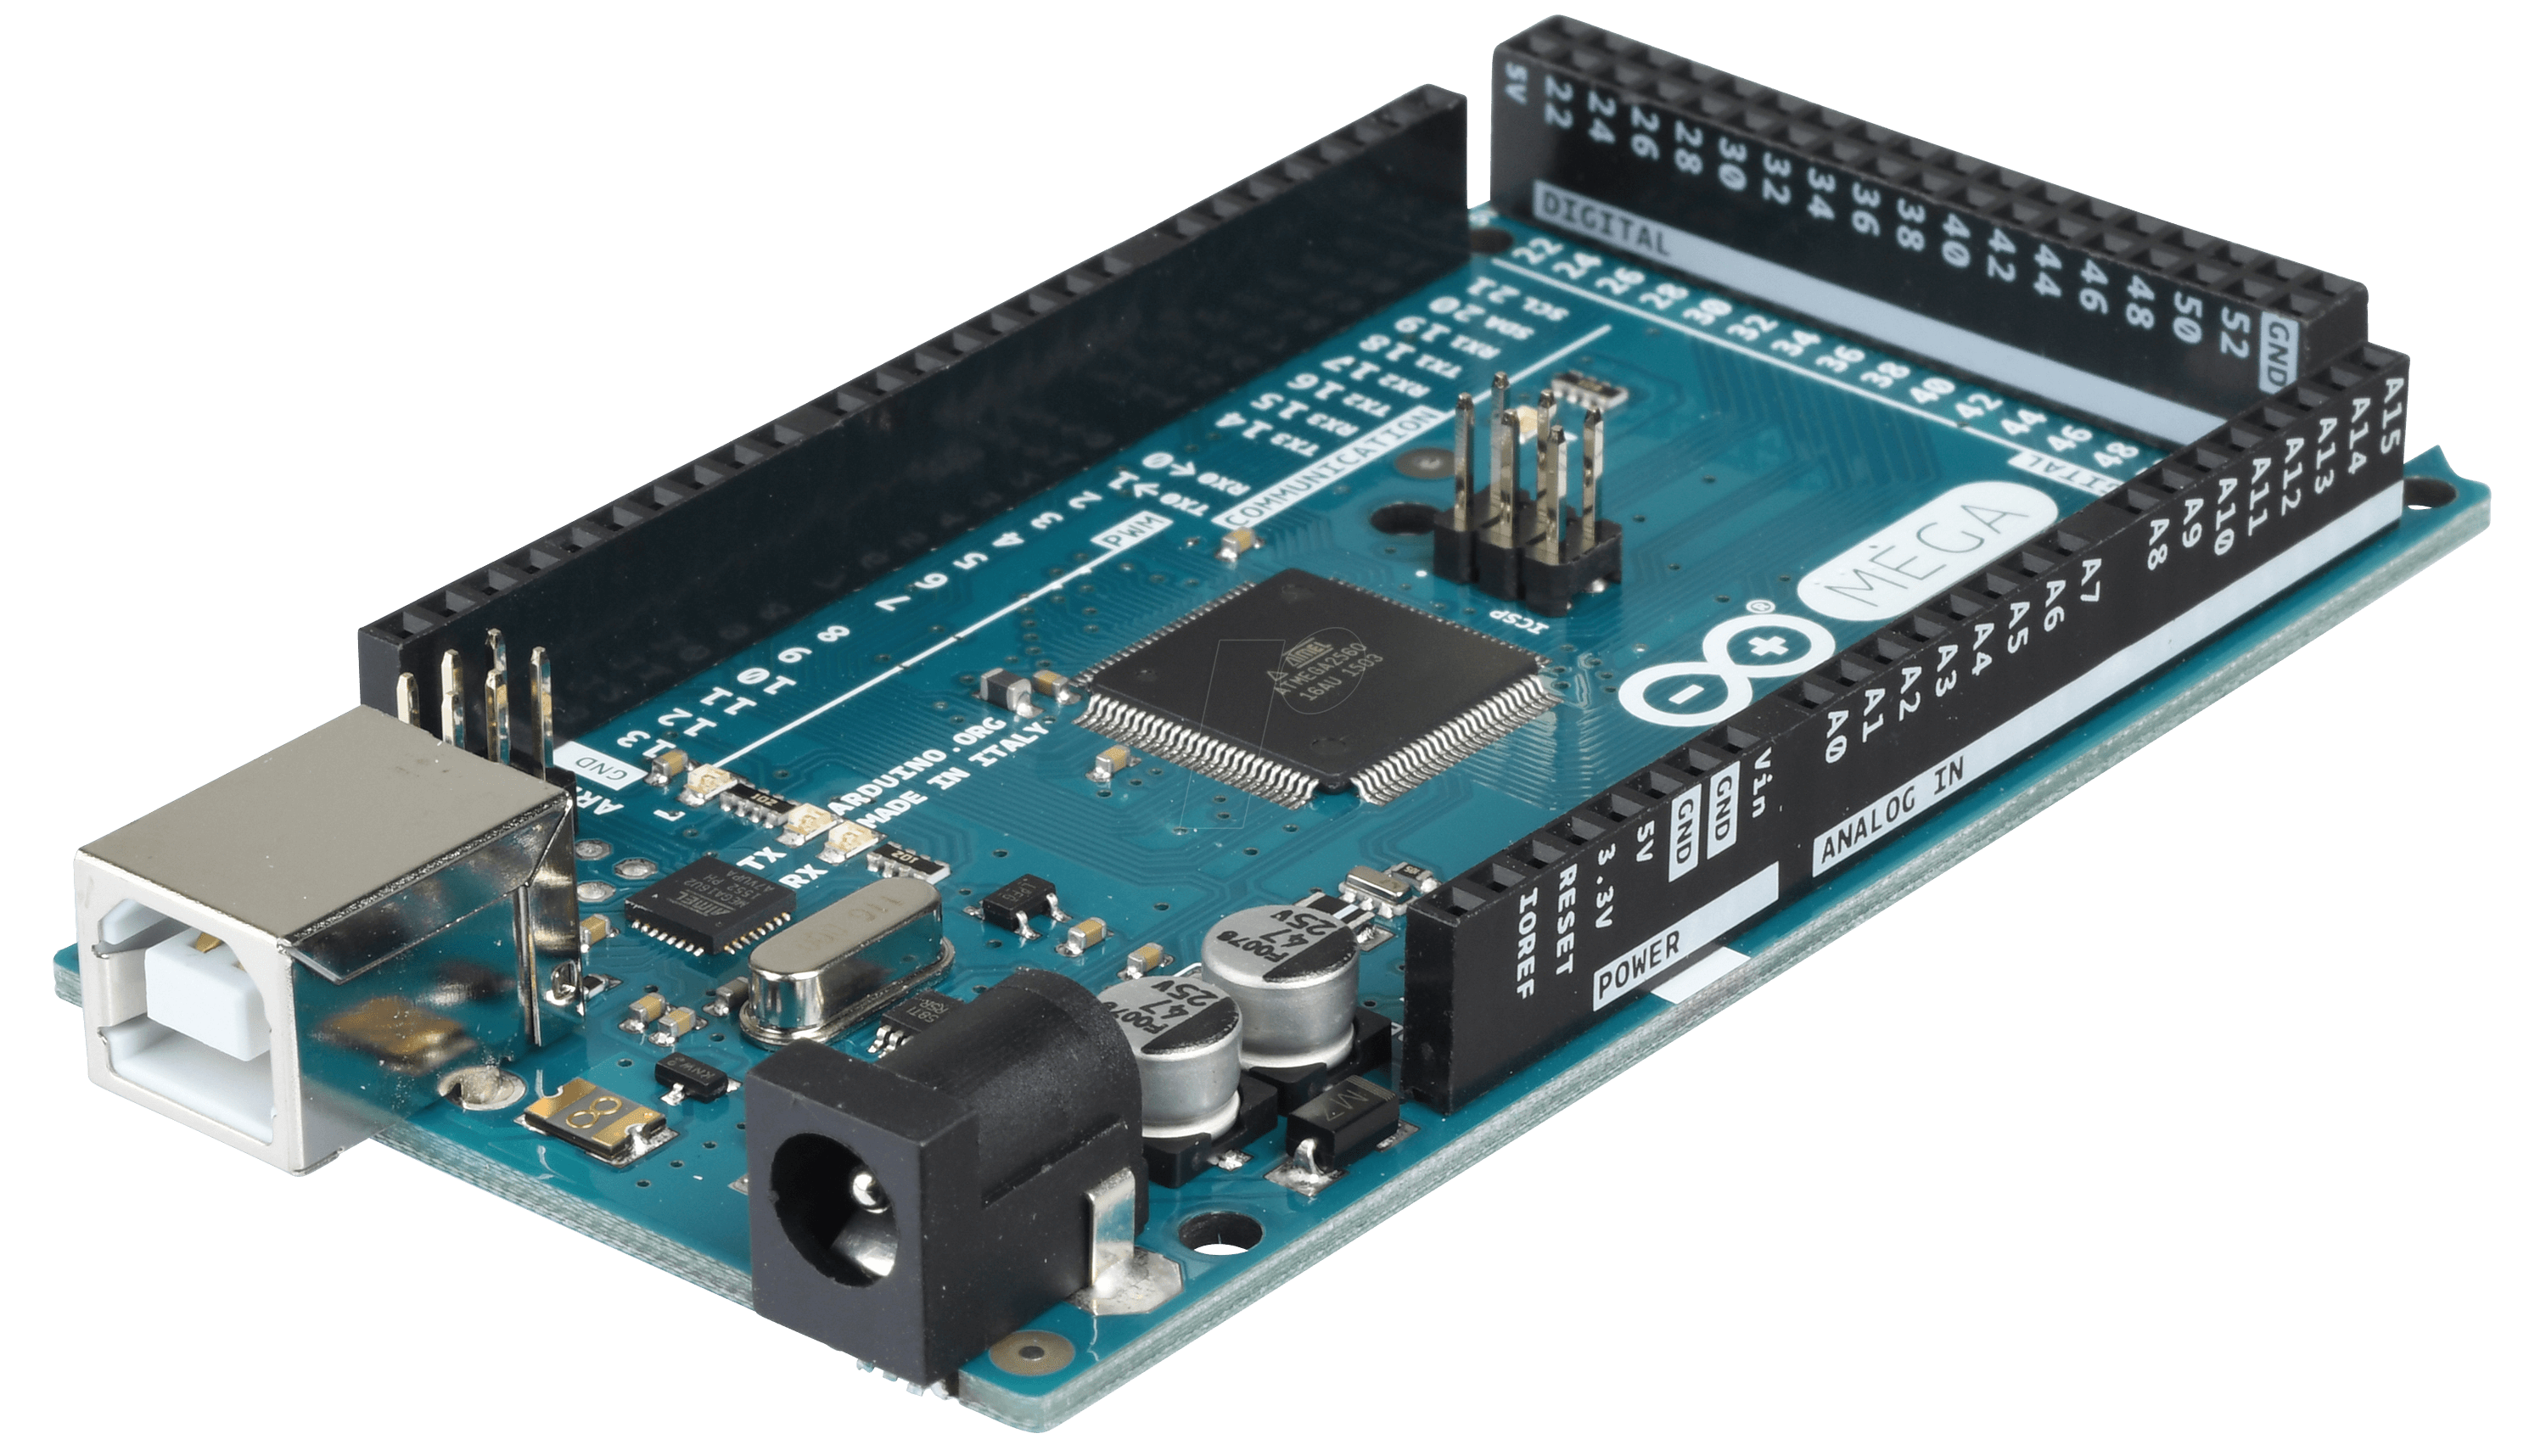
\includegraphics[width=14cm,height=10cm]{figure_t}
	\caption{Arduino Mega 25600}
	\label{figure_t}
\end{figure}

\subsection{Servo interface}
We want to make a servo interface with the arduino mega and that would make installing the servos so easy without making a mess. In theory we could use 48 servos on a Mega board, but we only soldered 18 servo ports, just to keep wires tidy and compact.

\begin{figure}[H]
	\centering
	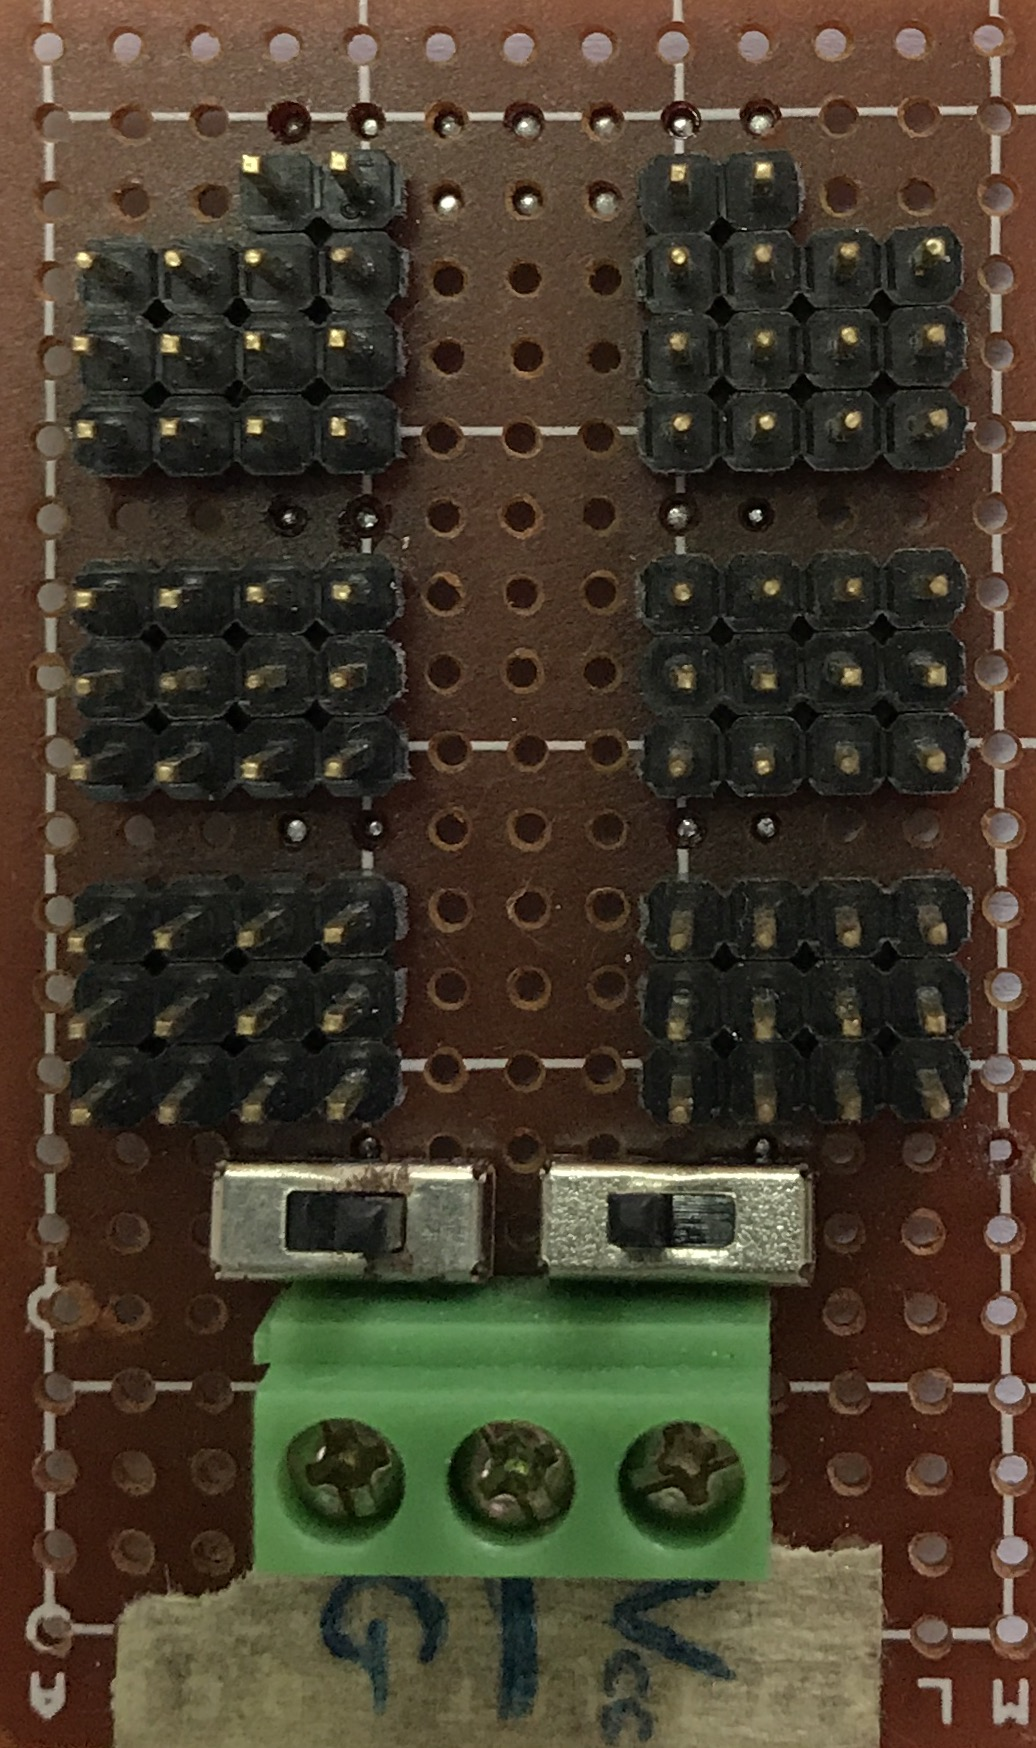
\includegraphics[width=4cm,height=6cm]{figure_u}
	\caption{Servo interface}
	\label{figure_u}
\end{figure}

\subsection{Raspberry Pi 3}
We used a Raspberry Pi 3 as an embedded computer to host our OS and to run ROS (Robotic Operating System). With the folllowing specs, Raspberry Pi is a very good choice for an embedded PC besides offering a set of GPIO pins as well.

\begin{figure}[H]
	\centering
	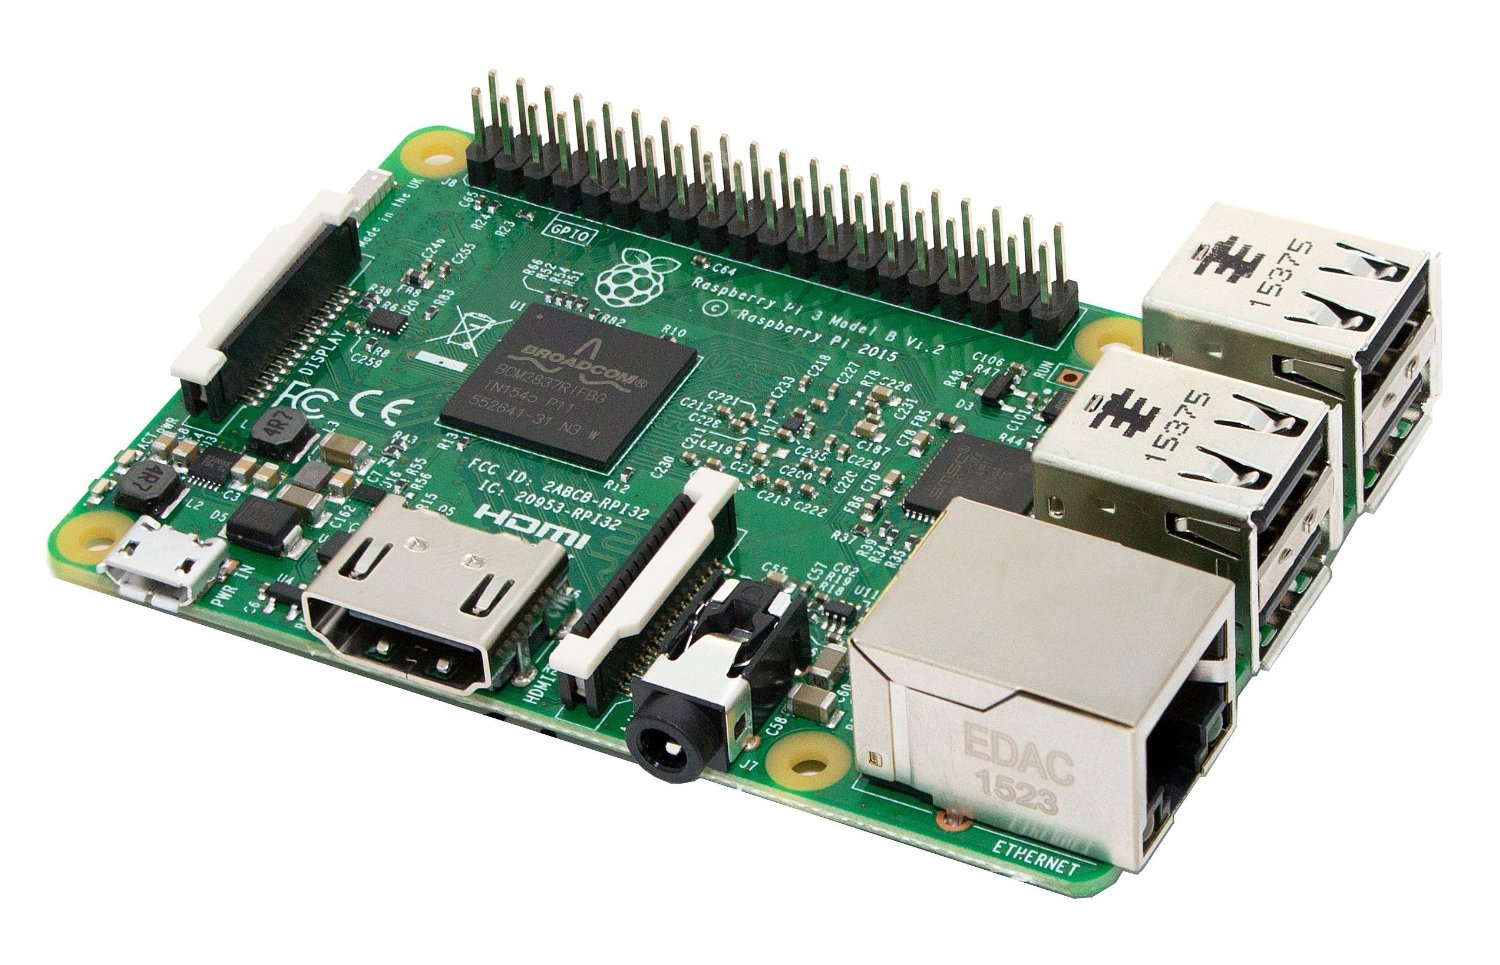
\includegraphics[width=9cm,height=5cm]{figure_v}
	\caption{Raspberry Pi 3 model B}
	\label{figure_v}
\end{figure}
\begin{center}
\begin{tabular}{ |l||p{12cm}|}
	\hline
	Processor      & Broadcom BCM2387 chipset. 1.2GHz Quad-Core ARM Cortex-A53 802.11 b/g/n Wireless LAN and Bluetooth 4.1 (Bluetooth Classic and LE)\\ \hline
	GPU               & Dual Core VideoCore IV® Multimedia Co-Processor. Provides Open GL ES 2.0, hardware-accelerated OpenVG, and 1080p30 H.264 high-profile decode. \\ \hline
	Memory          & 1GB LPDDR2  \\ \hline
	Operating System  & Boots from Micro SD card, running a version of the Linux operating system  \\ \hline
	Dimensions     & 85 x 56 x 17mm  \\ \hline
	Power             & Micro USB socket 5V1, 2.5A  \\ \hline
	Ethernet          & 10/100 BaseT Ethernet socket  \\ \hline
	Video Output   & HDMI (rev 1.3 \& 1.4 Composite RCA (PAL and NTSC)  \\ \hline
	Audio Output   & Audio Output 3.5mm jack, HDMI     \\ \hline
	USB                 & 4 x USB 2.0 Connector   \\ \hline
	GPIO Connector    & 40-pin 2.54 mm (100 mil) expansion header: 2x20 strip Providing 27 GPIO pins as well as +3.3 V, +5 V and GND supply lines \\ \hline
	Camera Connector  & 15-pin MIPI Camera Serial Interface (CSI-2) \\ \hline
	Display Connector & Display Serial Interface (DSI) 15 way flat flex cable connector with two data lanes and a clock lane    \\ \hline
	Memory Card       & Slot Push/pull Micro SDIO  \\ \hline
\end{tabular}
\end{center}


\subsection{NIMH battery}
We used a 5 volts NIMH battery to power up servo motors. With 1500 mAh capacity, ZagHexa is able to run for about 15 minutes.

\begin{figure}[H]
	\centering
	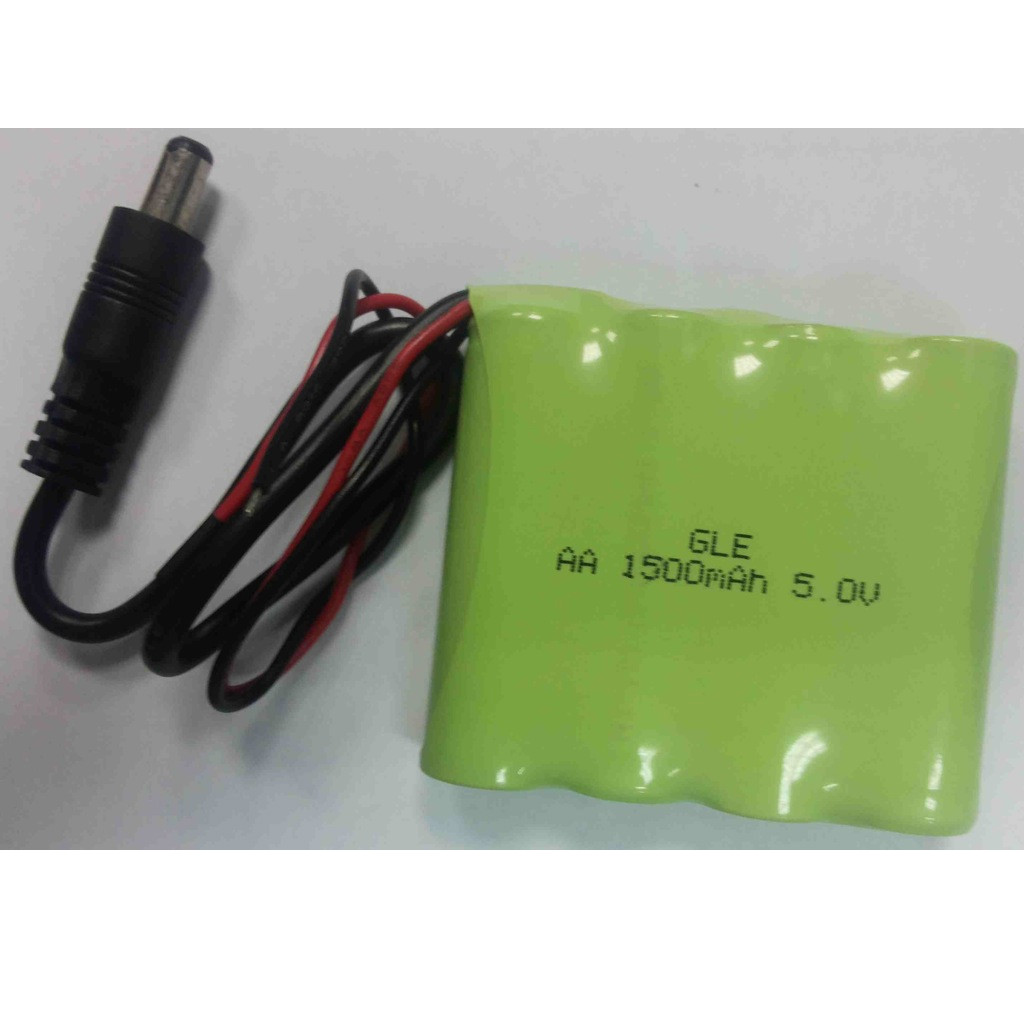
\includegraphics[width=8cm,height=5cm]{figure_w}
	\caption{5V NIMH battery}
	\label{figure_w}
\end{figure}

%%%%%%%%%%%%%%%%%%%%%%%%%%%%%%%%%%%%%%%%%%%%%%%%%%%%%%%%%%%%%%%%%%%%%%%%%%%%%%%
\setchapterpreamble[o]{%
	\dictum[Steve jobs, \textit{(businessman, inventor,Apple CEO, 1955--2011)}]{% source: https://www.brainyquote.com/quotes/quotes/s/stevejobs416875.html
		``You can't connect the dots looking forward; you can only connect them looking backwards. So you have to trust that the dots will somehow connect in your future. You have to trust in something - your gut, destiny, life, karma, whatever. This approach has never let me down, and it has made all the difference in my life.''}\vspace{0.1em}}

\chapter{Software Architecture}\label{ch:SoftwareArchitecture}
%{Software Architecture }

The high–level functionality and control of the robot are implemented in ROS packages. The Robot Operating System (ROS) is a standard and open–source operating system for robot control \cite{9}. ROS is not an operating system in the traditional sense of process management and scheduling; rather, it provides a structured communication layer above the host operating systems of a heterogeneous compute cluster. Our software ROS packages interact with each of the subsystems in C++ and Python for direct system control. The system described uses a Linux based software framework as an operating system (OS) for providing the advantages of using an OS, which supports developing additional modules that can be easily implemented and integrated. 

\section{Robot Operating System (ROS)}

Robot Operating System (ROS) provides operating system like service for the robot. It is a meta-operating system, which loads on top of an operating system, including hardware abstraction, low-level device control, implementation of commonly-used functionality, message-passing between processes, and package management. It also provides tools and libraries for obtaining, building, writing, and running code across multiple computers. These facilities cannot only help robots but also other embedded systems with a rich set of tools to successfully manage the complexity. With ROS handling the basic communications and data exchange.

ROS currently only runs on Unix-based platforms. Software for ROS is primarily tested on Ubuntu and Mac OS X systems, though the ROS community has been contributing support for Fedora, Gentoo, Arch Linux and other Linux platforms. While a port to Microsoft Windows for ROS is possible, it has not yet been fully explored.

The core ROS system, along with useful tools and libraries are regularly released as a ROS Distribution. This distribution is similar to a Linux distribution and provides a set of compatible software for others to use and build upon example for this distribution: Hydro, Indigo, Jade, Kinetic, Lunar...etc. [http://wiki.ros.org]

Our choice was Kinetic because is the update  distribution that have a LTS with high variety of support from ROS community that make it easy to exchange the knowledge and figure out how to solve issues and to come up with new idea to implement it. 
\subsection{Why ROS?}
	The answer for this question lies in power of ROS the make it preferable for most of the designers: 
  
	\begin{description}
		\item [Inter-platform operability]: ROS message-passing means that you can work between very different components and subsystems that are probably running with different languages (maybe something like low-level hardware control with C for speed, and high-level state machines with Java or Python for ease of coding). This also gets around the problem of the mess of APIs you would have had to deal with before.
		
		\item [Modularity]: Since things are connected by a distributed message system, if one component crashes, your whole system doesn't crash. Granted, there are plenty of ways to make your system more robust so that this doesn't happen in the first place, but ROS makes it easier for your robot to continue doing its thing even if two sensors and an arm motor have died (for example).
		
		\item [Concurrent resource handling]: Without ROS, reading/writing to resources quickly becomes a mess with large multi-threaded systems (i.e. virtually any robotics application). Again, there are ways to deal with this, but ROS simplifies the whole process by ensuring that your threads aren't actually trying to read and write to shared resources, but are rather just publishing and subscribing to messages.
		\item[ Vibrant Community]: Over the past several years, ROS has grown to include a large community of users worldwide. Historically, the majority of the users were in research labs, but increasingly we are seeing adoption in the commercial sector, particularly in industrial and service robotics.
		
		\item [Collaborative Environment]: ROS by itself offers a lot of value to most robotics projects, but it also presents an opportunity to network and collaborate with the world class roboticists that are part of the ROS community. One of the core philosophies in ROS is shared development of common components.
	\end{description}
Interested reader can find more information,material, and much more at:  \url{www.ros.org/core-components}

\subsection{ROS Package}
	Software in ROS is organized in packages. A package might contain ROS nodes, a ROS-independent library, a dataset, configuration files, a third-party piece of software, or anything else that logically constitutes a useful module. The goal of these packages it to provide this useful functionality in an easy-to-consume manner so that software can be easily reused. In general, ROS packages follow a "Goldilocks" principle: enough functionality to be useful, but not too much that the package is heavyweight and difficult to use from other software.
	
	Packages are easy to create by hand or with tools like catkin\_create\_pkg. A ROS package is simply a directory descended from ROS\_PACKAGE\_PATH (see ROS Environment Variables) that has a package.xml file in it. Packages are the most atomic unit of build and the unit of release. This means that a package is the smallest individual thing you can build in ROS and it is the way software is bundled for release (meaning, for example, there is one debian package for each ROS package), respectively.
	
\subsection{ROS Node}
	
	A node is a process that performs computation. Nodes are combined together into a graph and communicate with one another using streaming topics, RPC services, and the Parameter Server. These nodes are meant to operate at a fine-grained scale; a robot control system will usually comprise many nodes. For example, one node controls a laser range-finder, one Node controls the robot's wheel motors, one node performs localization, one node performs path planning, one node provide a graphical view of the system, and so on.
	
	The use of nodes in ROS provides several benefits to the overall system. There is additional fault tolerance as crashes are isolated to individual nodes. Code complexity is reduced in comparison to monolithic systems. Implementation details are also well hidden as the nodes expose a minimal API to the rest of the graph and alternate implementations, even in other programming languages, can easily be substituted.
	
	All running nodes have a graph resource name that uniquely identifies them to the rest of the system. For example, /hokuyo\_node could be the name of a Hokuyo driver broadcasting laser scans. Nodes also have a node type, that simplifies the process of referring to a node executable on the fileystem. These node types are package resource names with the name of the node's package and the name of the node executable file. In order to resolve a node type, ROS searches for all executables in the package with the specified name and chooses the first that it finds. As such, you need to be careful and not produce different executables with the same name in the same package. Finally, a ROS node is written with the use of a ROS client library, such as roscpp or rospy.
	
\subsection{Publisher/Subscriber}
	The Publisher object represents a publisher on the ROS network. The object publishes to an available topic or to a topic that it creates. This topic has an associated message type. When the Publisher object publishes a message to the topic, all subscribers to the topic receive this message. The same topic can have multiple publishers and subscribers.
	
	The primary mechanism for ROS nodes to exchange data is to send and receive messages. Messages are transmitted on a topic and each topic has a unique name in the ROS network. If a node wants to share information, it will use a publisher to send data to a topic. A node that wants to receive that information will use a subscriber to that same topic. Besides its unique name, each topic also has a message type, which determines the types of messages that are allowed to be transmitted.
	
	This publisher/subscriber communication has the following characteristics:
	\begin{enumerate}
		\item Topics are used for many-to-many communication. Many publishers can send messages to the same topic and many subscribers can receive them.
		\item Publisher and subscribers are decoupled through topics and can be created and destroyed in any order. A message can be published to a topic even if there are no active subscribers.
	\end{enumerate}
	
	The concept of topics, publishers, and subscribers is illustrated in the figure.\ref{Pub}.
	\begin{figure}[h]		
		\centering
		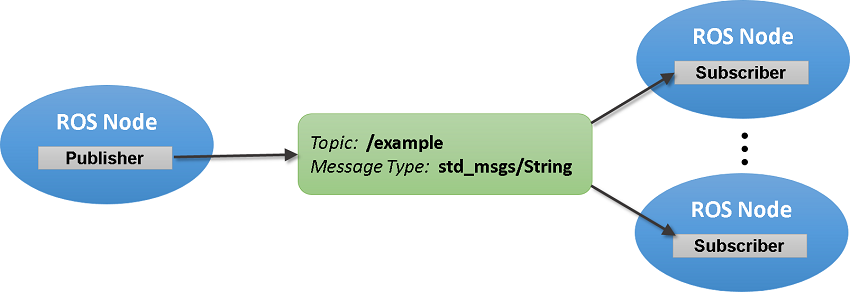
\includegraphics[width =.8\textwidth]{publish_subscribe_concept}
		\caption{publish subscribe concept}
		\label{Fig:Pub}
	\end{figure}


\subsection{ROS Topic}

	Topics are named buses over which nodes exchange messages. Topics have anonymous publish/subscribe semantics, which decouples the production of information from its consumption. In general, nodes are not aware of who they are communicating with. Instead, nodes that are interested in data subscribe to the relevant topic; nodes that generate data publish to the relevant topic. There can be multiple publishers and subscribers to a topic.
	
	Topics are intended for unidirectional, streaming communication. Nodes that need to perform remote procedure calls, i.e. receive a response to a request, should use services instead. There is also the Parameter Server for maintaining small amounts of state.
	
	Each topic is strongly typed by the ROS message type used to publish to it and nodes can only receive messages with a matching type. The Master does not enforce type consistency among the publishers, but subscribers will not establish message transport unless the types match. Furthermore, all ROS clients check to make sure that an MD5 computed from the msg files match. This check ensures that the ROS Nodes were compiled from consistent code bases.
	
	with a simple words we can define this terms:\\
	
	Nodes: A node is an executable that uses ROS to communicate with other nodes.
	Topics: Nodes can publish messages to a topic as well as subscribe to a topic to receive messages.
	Messages: ROS data type used when subscribing or publishing to a topic.
	Master: The ROS Master provides name registration and lookup to the rest of the Computation Graph. Without the Master, nodes would not be able to find each other, exchange messages, or invoke services.
	roscore: is a collection of nodes and programs that are pre-requisites of a ROS-based system. You must have a roscore running in order for ROS nodes to communicate. It is launched using the roscore command.
	
	

\subsection{Can we access ROS form a remote computer?}
	ROS is a distributed computing environment. A running ROS system can comprise dozens, even hundreds of nodes, spread across multiple machines. Depending on how the system is configured, any node may need to communicate with any other node, at any time.	
	\begin{itemize}
		\item There must be complete, bi-directional connectivity between all pairs of machines, on all ports.
		\item Each machine must advertise itself by a name that all other machines can resolve.
	\end{itemize}

More information can be found at:  \url{wiki.ros.org/ROS/NetworkSetup}

\section{UNIX}
	UNIX is an open source operating system which was first developed in the 1960s, and has been under constant development ever since. By operating system, we mean the suite of programs which make the computer work. It is a stable, multi-user, multi-tasking system for servers, desktops and laptops.
	UNIX systems also have a graphical user interface (GUI) similar to Microsoft Windows which provides an easy to use environment. However, knowledge of UNIX is required for operations which aren't covered by a graphical program, or for when there is no windows interface available.
	
	- Types of UNIX
	
	There are many different versions of UNIX, although they share common similarities. The most popular varieties of UNIX are Sun Solaris, GNU/Linux, Ubuntu, Kali, and MacOS X.
	Here in the School, we use Solaris on our servers and workstations, and Fedora Linux on the servers and desktop PCs.
	
	- The UNIX operating system
	The UNIX operating system is made up of three parts; the kernel, the shell and the programs.
	
	- The kernel
	The kernel of UNIX is the hub of the operating system: it allocates time and memory to programs and handles the filestore and communications in response to system calls.
	
	- The shell
	The shell acts as an interface between the user and the kernel. The shell is a command line interpreter (CLI), it interprets the commands the user types in and arranges for them to be carried out.
	

\section{General View Of The Control System}

The control system of the robot can be divided into two parts:

\begin{itemize}
\item Raspberry Pi - High level -
\item Arduino - Low level -
\end{itemize}

All computing and control operation is done on RPi and Arduino that lies on the robot to inure the speed of control and precision.
The sensors data send from mobile App to the RPi through TCP/IP connection and to a computer also, RPi receive this data and process it to be aware with its environment and make a decision upon it, the computer show this data on a GUI to the operator/user so he can also make a decision using the reading form sensors and the camera.
When a order form an operator using Joystick/Bluetooth to move the robot the RPi take this order and send it to the Arduino through a serial port, using a C++ program in Arduino we compute the angles to move to the desired direction with minimal error. Figure\ref{Fig:Outline} show an Outline for the control system.

\begin{figure}[h]		
	\centering
	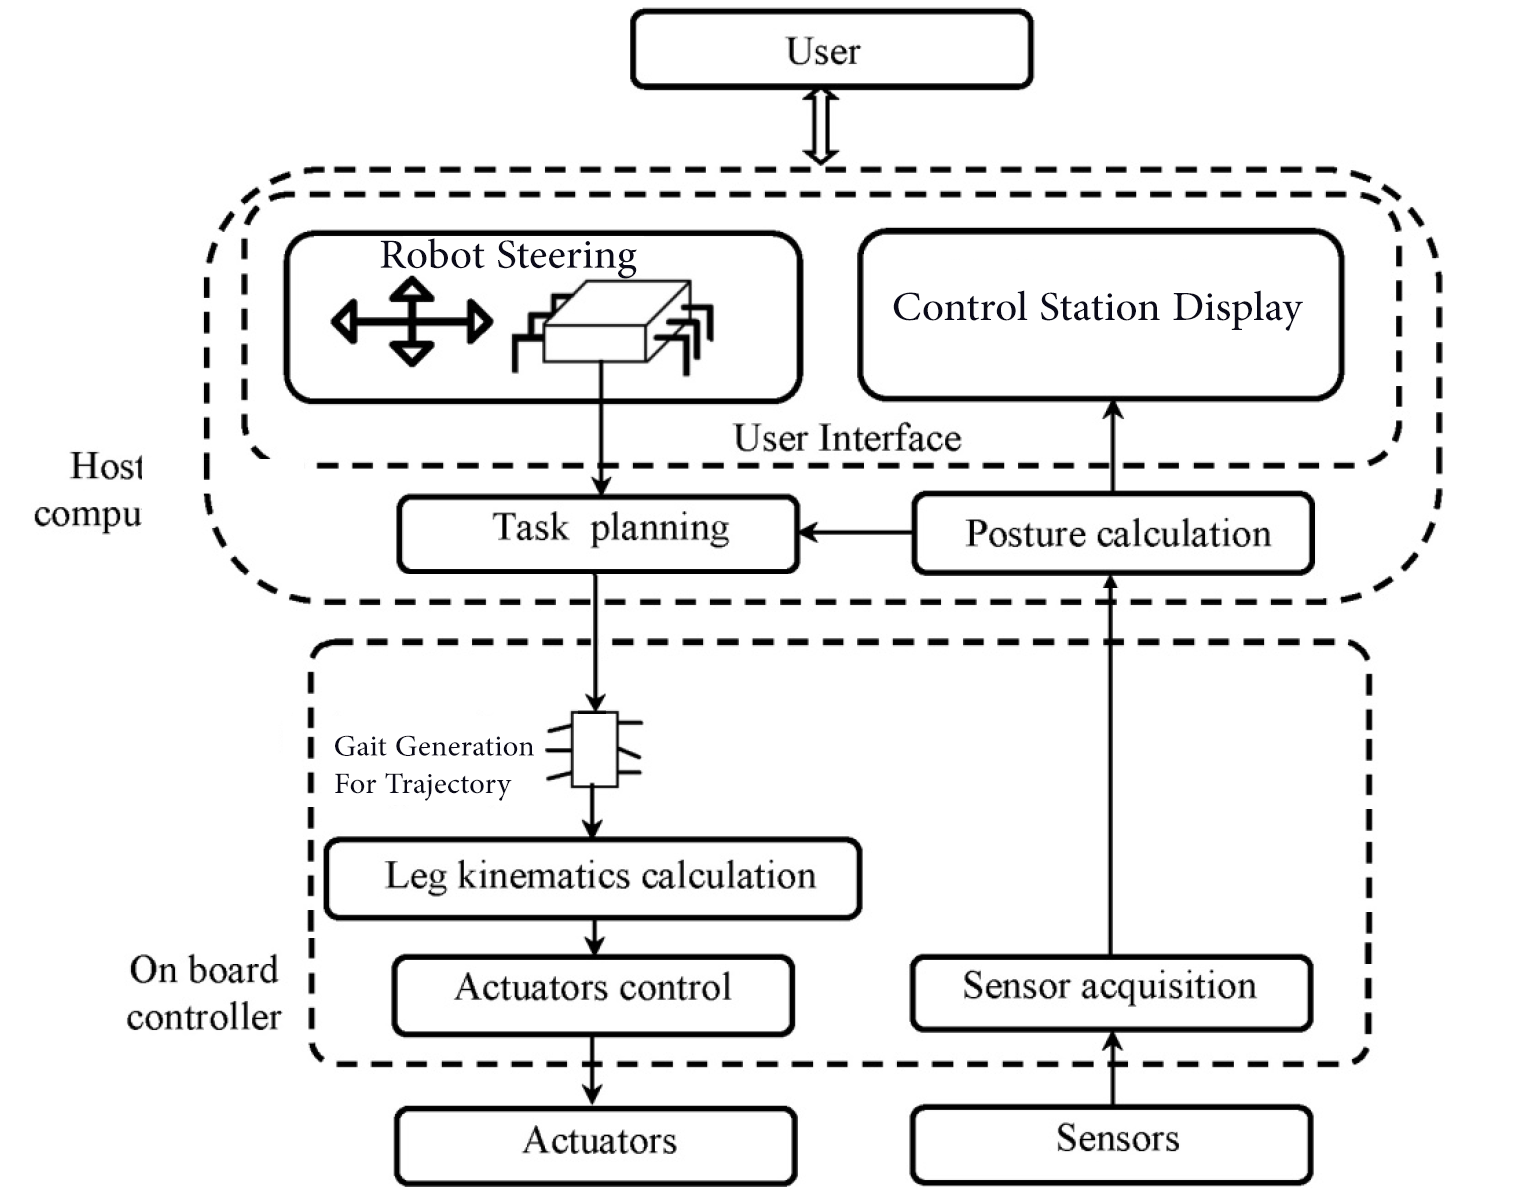
\includegraphics[width =.8\textwidth]{OCS}
	\caption{Outline of control systems.}
	\label{Fig:Outline}
\end{figure}


\subsection{Raspberry Pi}

A Raspberry Pi is a credit card-sized computer originally designed for education, inspired by the 1981 BBC Micro. Creator Eben Upton's goal was to create a low-cost device that would improve programming skills and hardware understanding. But thanks to its small size and accessible price, it was quickly adopted by tinkerers, makers, and electronics enthusiasts for projects that require more than a basic microcontroller.

The Raspberry Pi is slower than a modern laptop or desktop but is still a complete Linux computer and can provide all the expected abilities that implies, at a low-power consumption level.

The Raspberry Pi is open hardware, with the exception of the primary chip on the Raspberry Pi, the Broadcomm SoC (System on a Chip), which runs many of the main components of the board–CPU, graphics, memory, the USB controller, etc. Many of the projects made with a Raspberry Pi are open and well-documented as well and are things you can build and modify yourself.

\begin{itemize}
	\item What kind of operating system does the Raspberry Pi run?\\
	
	The Raspberry Pi was designed for the Linux operating system, and many Linux distributions now have a version optimized for the Raspberry Pi.
	
	Two of the most popular options are Raspbian, which is based on the Debian operating system, and Pidora, which is based on the Fedora operating system. For beginners, either of these two work well; which one you choose to use is a matter of personal preference. A good practice might be to go with the one which most closely resembles an operating system you’re familiar with, in either a desktop or server environment.
	
	If you would like to experiment with multiple Linux distributions and aren't sure which one you want, or you just want an easier experience in case something goes wrong, try NOOBS, which stands for New Out Of Box Software. When you first boot from the SD card, you will be given a menu with multiple distributions (including Raspbian and Pidora) to choose from. If you decide to try a different one, or if something goes wrong with your system, you simply hold the Shift key at boot to return to this menu and start over.
	
	There are, of course, lots of other choices. OpenELEC and RaspBMC are both operating system distributions based on Linux that are targeted towards using the Raspberry Pi as a media center. There are also non-Linux systems, like RISC OS, which run on the Pi. Some enthusiasts have even used the Raspberry Pi to learn about operating systems by designing their own.
\end{itemize}

% Take this to the Component Part 
	Raspberry Pi 3 Model B specification
	The Raspberry Pi 3 Model B is the third generation Raspberry Pi. This powerful credit-card sized single board computer can be used for many applications and supersedes the original Raspberry Pi Model B+ and Raspberry Pi 2 Model B. Whilst maintaining the popular board format the Raspberry Pi 3 Model	B brings you a more powerful processer, 10x faster than the first generation Raspberry Pi. Additionally it adds wireless LAN \& Bluetooth connectivity making it the ideal solution for powerful connected designs.
\begin{figure}[h]
\centering
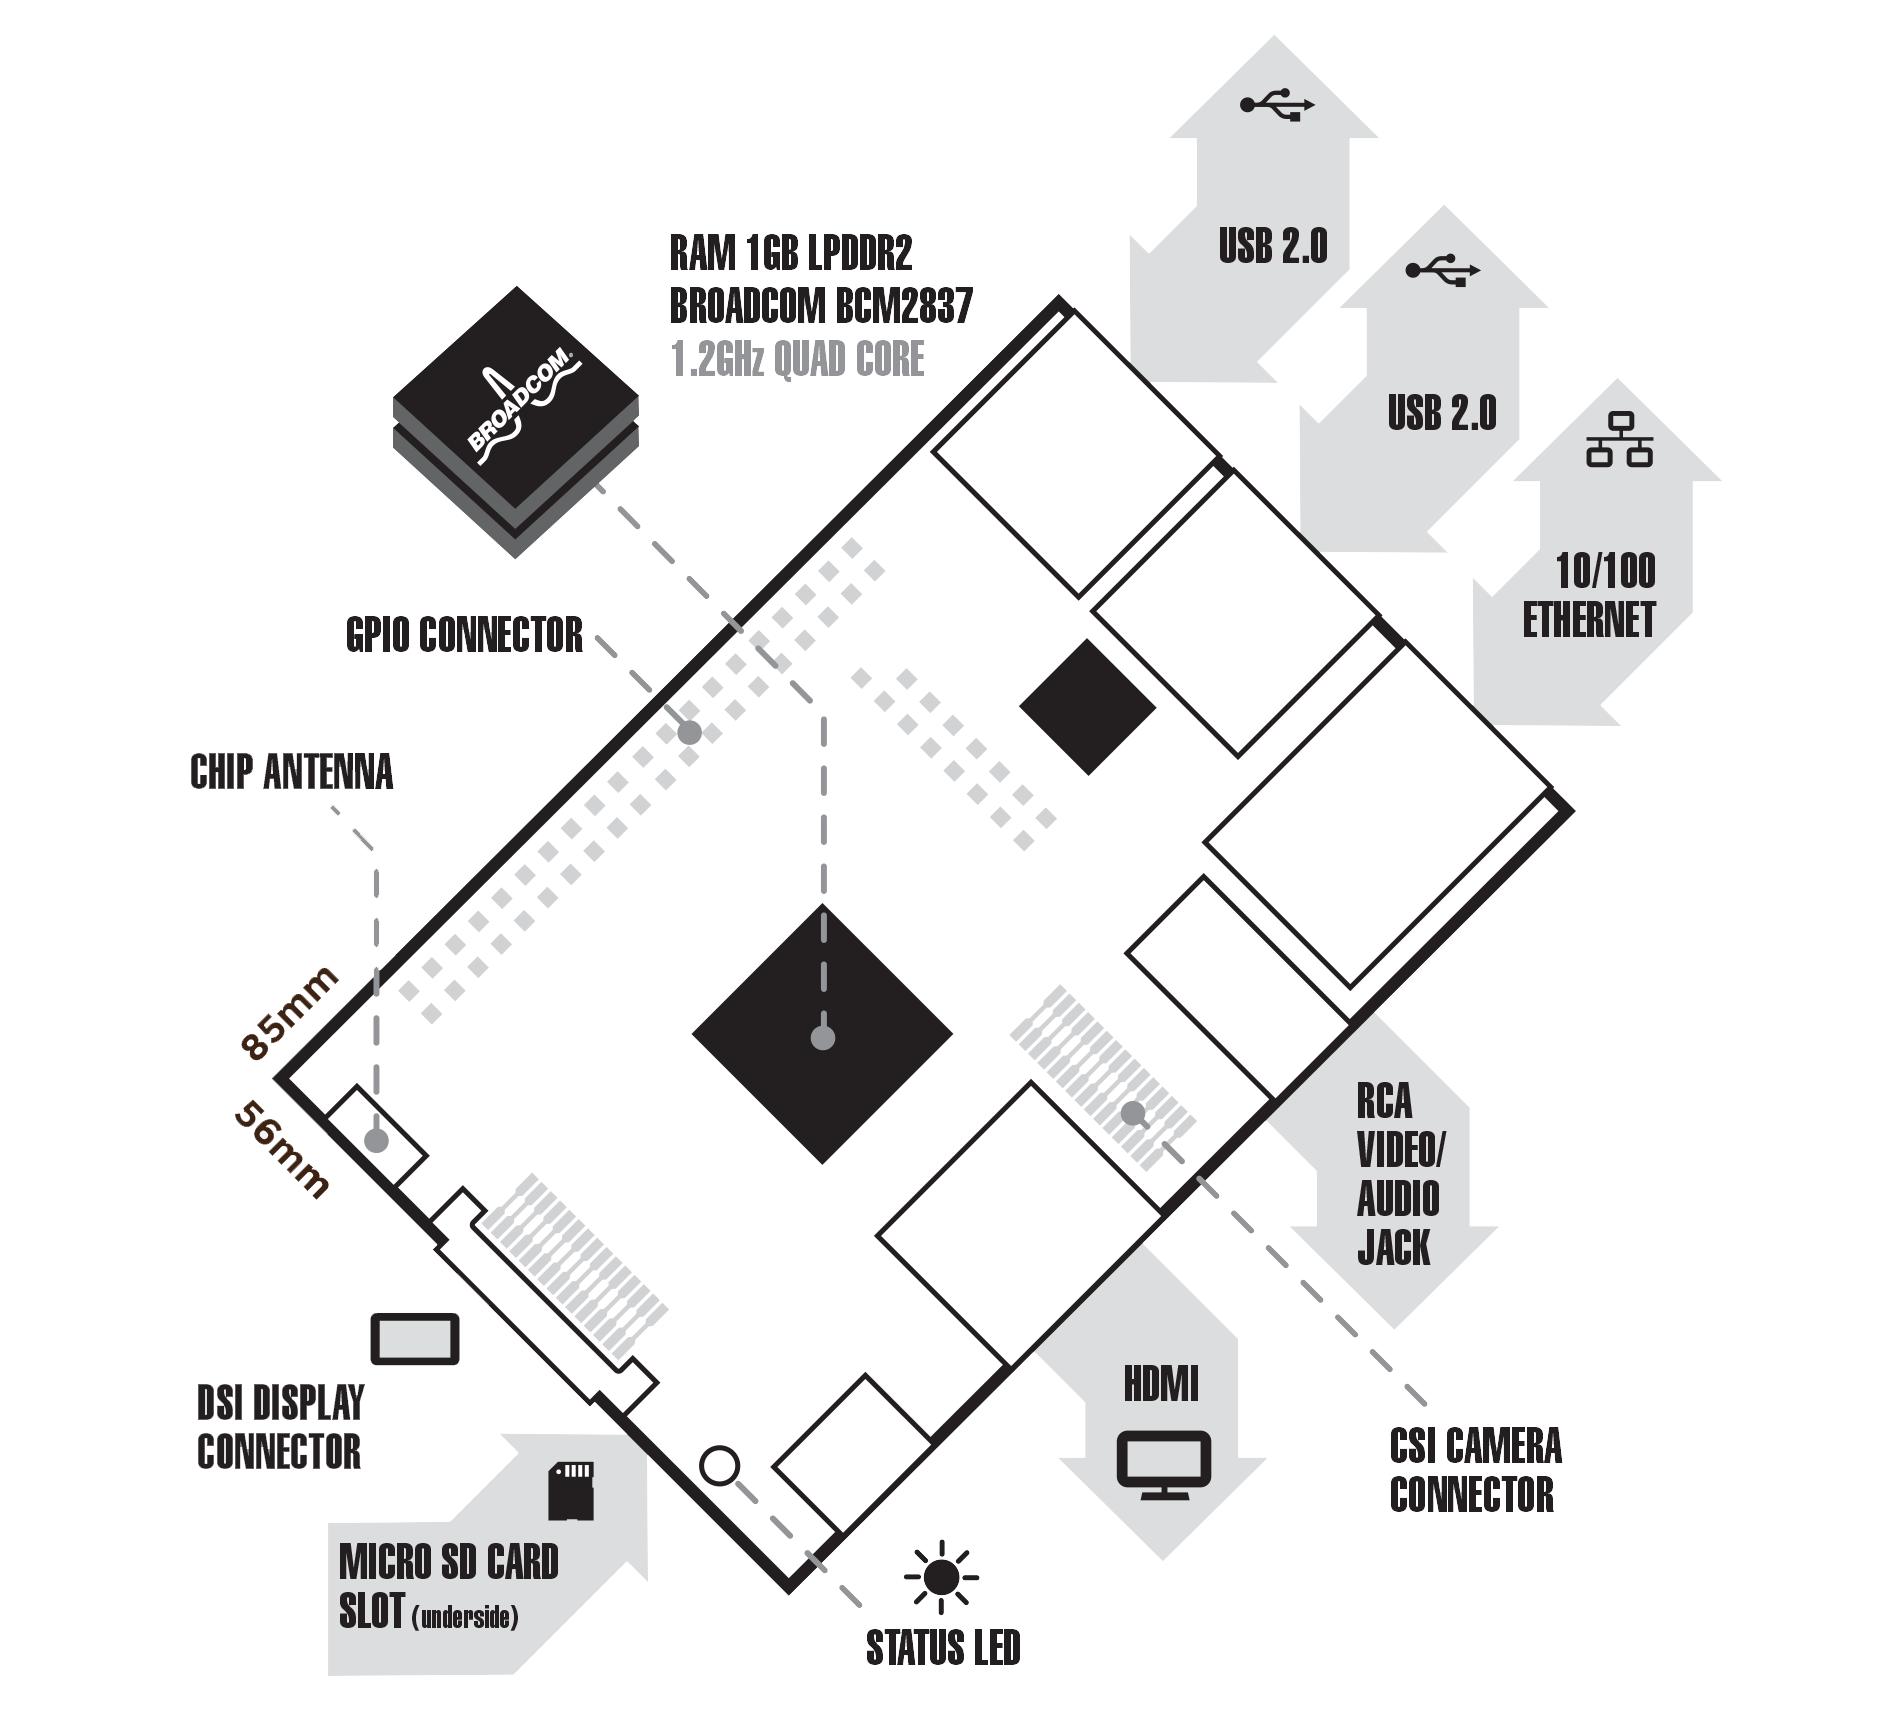
\includegraphics[width =.8\textwidth]{RP3}
\caption{Raspberry Pi 3 Model B.}
\label{Fig:RP3}
\end{figure}
\begin{center}
\begin{tabular}{ |l||p{12cm}|}
	\hline
	Processor      & Broadcom BCM2387 chipset. 1.2GHz Quad-Core ARM Cortex-A53 802.11 b/g/n Wireless LAN and Bluetooth 4.1 (Bluetooth Classic and LE)\\ \hline
	GPU               & Dual Core VideoCore IV® Multimedia Co-Processor. Provides Open GL ES 2.0, hardware-accelerated OpenVG, and 1080p30 H.264 high-profile decode. \\ \hline
	Memory          & 1GB LPDDR2  \\ \hline
	Operating System  & Boots from Micro SD card, running a version of the Linux operating system  \\ \hline
	Dimensions     & 85 x 56 x 17mm  \\ \hline
	Power             & Micro USB socket 5V1, 2.5A  \\ \hline
	Ethernet          & 10/100 BaseT Ethernet socket  \\ \hline
	Video Output   & HDMI (rev 1.3 \& 1.4 Composite RCA (PAL and NTSC)  \\ \hline
	Audio Output   & Audio Output 3.5mm jack, HDMI     \\ \hline
	USB                 & 4 x USB 2.0 Connector   \\ \hline
	GPIO Connector    & 40-pin 2.54 mm (100 mil) expansion header: 2x20 strip Providing 27 GPIO pins as well as +3.3 V, +5 V and GND supply lines \\ \hline
	Camera Connector  & 15-pin MIPI Camera Serial Interface (CSI-2) \\ \hline
	Display Connector & Display Serial Interface (DSI) 15 way flat flex cable connector with two data lanes and a clock lane    \\ \hline
	Memory Card       & Slot Push/pull Micro SDIO  \\ \hline
\end{tabular}
\end{center}

	\subsubsection{Ubuntu MATE with Raspberry Pi}
	Ubuntu MATE is a stable, easy-to-use operating system with a configurable desktop environment. It is ideal for those who want the most out of their computers and prefer a traditional desktop metaphor. With modest hardware requirements it is suitable for modern workstations, single board computers and older hardware alike. Ubuntu MATE makes modern computers fast and old computers usable.
	
	The MATE desktop is essentially a continuation of the traditional Gnome 2 desktop environment. Combining the MATE desktop with Ubuntu gives you an experience that is almost identical to the early days of Ubuntu, prior to the switch to Unity.
	
	Martin Wimpress and Rohith Madhavan have made an Ubuntu MATE image for the Raspberry Pi 2 and Raspberry Pi 3 based on the regular Ubuntu armhf base, not the new Ubuntu “Snappy” Core, which means that the installation procedure for applications uses the traditional tools, ie apt-get with highly recommended microSDHC Class 6 or Class 10 microSDHC card. Ubuntu MATE 16.04 also fully supports the built-in Bluetooth and Wifi on the Raspberry Pi 3 and features hardware accelerated video playback in VLC and hardware accelerated decoding and encoding in ffmpeg
	
	To installing Ubuntu MATE onto Raspberry Pi 3, starting by download the OS into microSD then the partition is automatically resized to fill your microSD card when the pi is powered up for the first time, typical guided installer is shown up. Installation takes several minutes and finally the system reboots and you arrive at the desktop. A Welcome app provides some good information on Ubuntu MATE, including a section specific for the Raspberry Pi.
	
	The Welcome app explains that the while the system is based on Ubuntu MATE and uses Ubuntu armhf base, it is in fact using the same kernel as Raspian. It also turns out that a whole set of Raspian software has been ported over such as raspi-config, rpi.gpio, sonic-pi, python-sent-hat, omxplayer, etc.
	
	[ubuntu-mate.org/blog/ubuntu-mate-xenial-raspberry-pi]
	
	\subsubsection{Raspberry Pi with ROS} 
	
	This part is consider as the the brain of the robot as it contain all the nodes of our robot that make it move and interact with its environment, we can divide our program to two main packages that will control all functions in our robot:
	
	\begin{enumerate}
		\item Movement package \\ 
			This package is responsible to handle the movement of the robot, as it takes the input form joystick/bluetooth and using node Joystick it publish the wanted button to the low level Hardware to do an action upon the received button.
			
			this package have tow nodes, the first one on the RPi which handle the joystick/bluetooth part of taking command, the second node is on Arduino which receive the command and handle the action of movement as wanted.
			
			An Extra topic is add to the Arduino node to handle the ultrasonic sensor reading for more known of the environments variables. 
			\begin{figure}[h]		
				\centering
				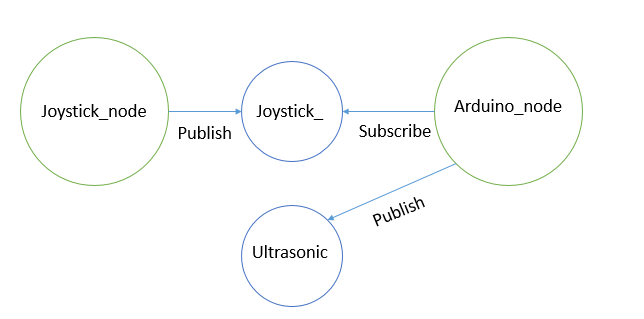
\includegraphics[width =.8\textwidth]{Movement_pck}
				\caption{General view of Movement Package.}
				\label{Fig:Movement}
			\end{figure}
		\item Client package  \\
			This package is responsible to handle the communication through the TCP/IP connection, this package is consist of two way of communication, so it receive the sensor data as will be descried in the Mobile Application section then it publish these data to the GUI node which can also select some sensor id or all sensors to be receive then publish it value to the Client node to git its value(s) form the mobile application.
			\begin{figure}[h]		
				\centering
				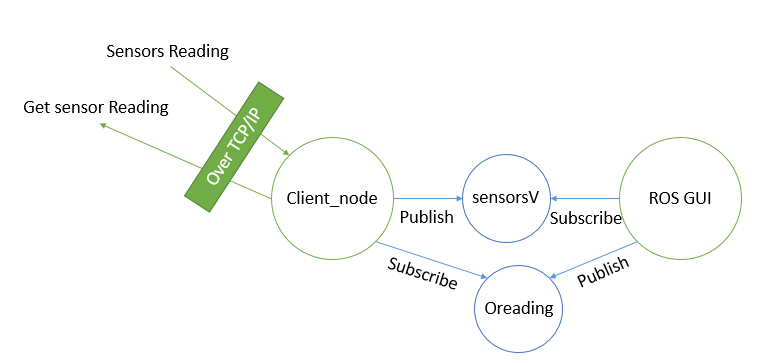
\includegraphics[width =.8\textwidth]{Client_pck}
				\caption{General view of Client Package.}
				\label{Fig:Client}
			\end{figure}  
	\end{enumerate}

\subsection{Arduino Mega}
Arduino is an open-source platform used for building electronics projects. Arduino consists of both a physical programmable circuit board (often referred to as a microcontroller) and a piece of software, or IDE (Integrated Development Environment) that runs on your computer, used to write and upload computer code to the physical board.

The Arduino platform has become quite popular with people just starting out with electronics, and for good reason. Unlike most previous programmable circuit boards, the Arduino does not need a separate piece of hardware (called a programmer) in order to load new code onto the board – you can simply use a USB cable. Additionally, the Arduino IDE uses a simplified version of C++, making it easier to program. 
Finally, Arduino provides a standard form factor that breaks out the functions of the micro-controller into a more accessible package.

The Arduino Mega 2560 is a microcontroller board based on the ATmega2560. It has 54 of digital input/output pins (14 can be used as PWM outputs), 16 analog inputs, a USB connection, a power jack,a 16 MHz crystal oscillator, and a reset button. It contains everything needed to support the microcontroller; simply connect it to a computer with a USB cable or power it with a AC-to-DC adapter or battery to get started. The large number of pins make this board very handy for projects that require a bunch of digital inputs or outputs.


\begin{figure}[h]		
	\centering
	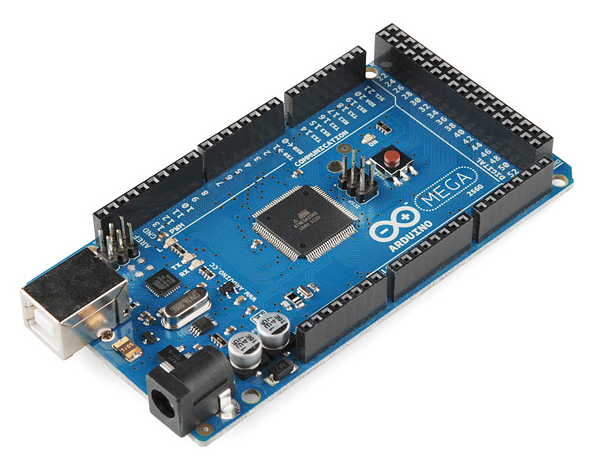
\includegraphics[width =.8\textwidth]{Arduino_Mega}
	\caption{Arduino Mega.}
	\label{Fig:Mega}
\end{figure}
	 Arduino Mega specification
\begin{center}
	\begin{tabular}{ |c|c|}
		\hline
		Microcontroller			& ATmega2560 \\ \hline
		Operating Voltage		& 5V\\ \hline
		Input Voltage			& (recommended) 7-12V\\ \hline
		Input Voltage (limits) 	& 6-20V\\ \hline
		Digital I/O Pins 		& 54 (of which 14 provide PWM output)\\ \hline
		Analog Input Pins 		& 16\\ \hline
		DC Current per I/O Pin	& 40 mA\\ \hline
		DC Current for 3.3V Pin & 50 mA\\ \hline
		Flash Memory			& 256 KB of which 8 KB used by bootloader\\ \hline
		SRAM					& 8 KB\\ \hline
		EEPROM 					& 4 KB\\ \hline
		Clock Speed 			& 16 MHz\\ \hline
	\end{tabular}
\end{center}

		\subsubsection{Arduino whit Raspberry Pi} 
		
		Rather than struggle with the very basic unprotected IO pins on the Raspberry Pi and the lack of real-time performance in Linux, the ideal setup for many real-world-interfacing projects is Raspberry Pi + Arduino.
		
		There are four basic ways to connect Arduino to Raspberry Pi:
		\begin{enumerate}
			\item Buy an add-on board like the Gertboard which has an Arduino compatible IC on it. Pricey.
			\item Plug a standard Arduino into the USB port of the RPi. This is by far the easiest method and minimises wiring and hassle. However it requires the more expensive Arduinos.
			\item Use a USB to Serial adapter with a cheaper/smaller Arduino like a Pro Mini or a self-made Shrimp. This is the best DIY option and has the same advantage of method 2 that you can power the Arduino/Shrimp from USB.
			\item Use the Serial Pins on the Raspberry Pi to connect to a cheaper/smaller Aruduino like a Pro Mini or a self-made Shrimp. This is theoretically the cheapest method but by far the most hassle. This is also the best method if you are using the cheaper Raspberry Pi Model A and its single USB port is being used for Wifi.
		\end{enumerate}	
		Using the second method to connect the two devices in serial connection,
		
		
		\subsubsection{Arduino PWM to Servo Motors} 
		
		
\section{Mobile Application}

	Most of the android devices have built-in sensors that measure motion, orientation, and various environmental condition.
	SensorsCORE is Android application act like server that read any kind of data from your smartphone's sensors and send it through socket request to any client.  
	
	- How to communicate: 
	
	The communication between SensorsCOER(server) and your application(client) based on socket communication. The server is accessed via server's IP address (or domain name) and a port number. Once two application are connected, they can communicate streams of bytes with each other.  
	
	- How it works: 
	
	Once your application connected with the server for the first time, it send a list of your available sensors in your smartphone - you can use – with its IDs. You can send ID of the desired sensor that you want to get its values to the server. Every time you send a request, you get an answer with the sensor values. So we have three type of requests. 
	The first request sent with first time connection with the list of available sensors and its IDs. 
	When you want a data form specific sensor, you sent a request with the sensor's id The third request is initialized when you want the data from all sensors. 

	Example:
	\begin{figure}[h]		
	\centering
	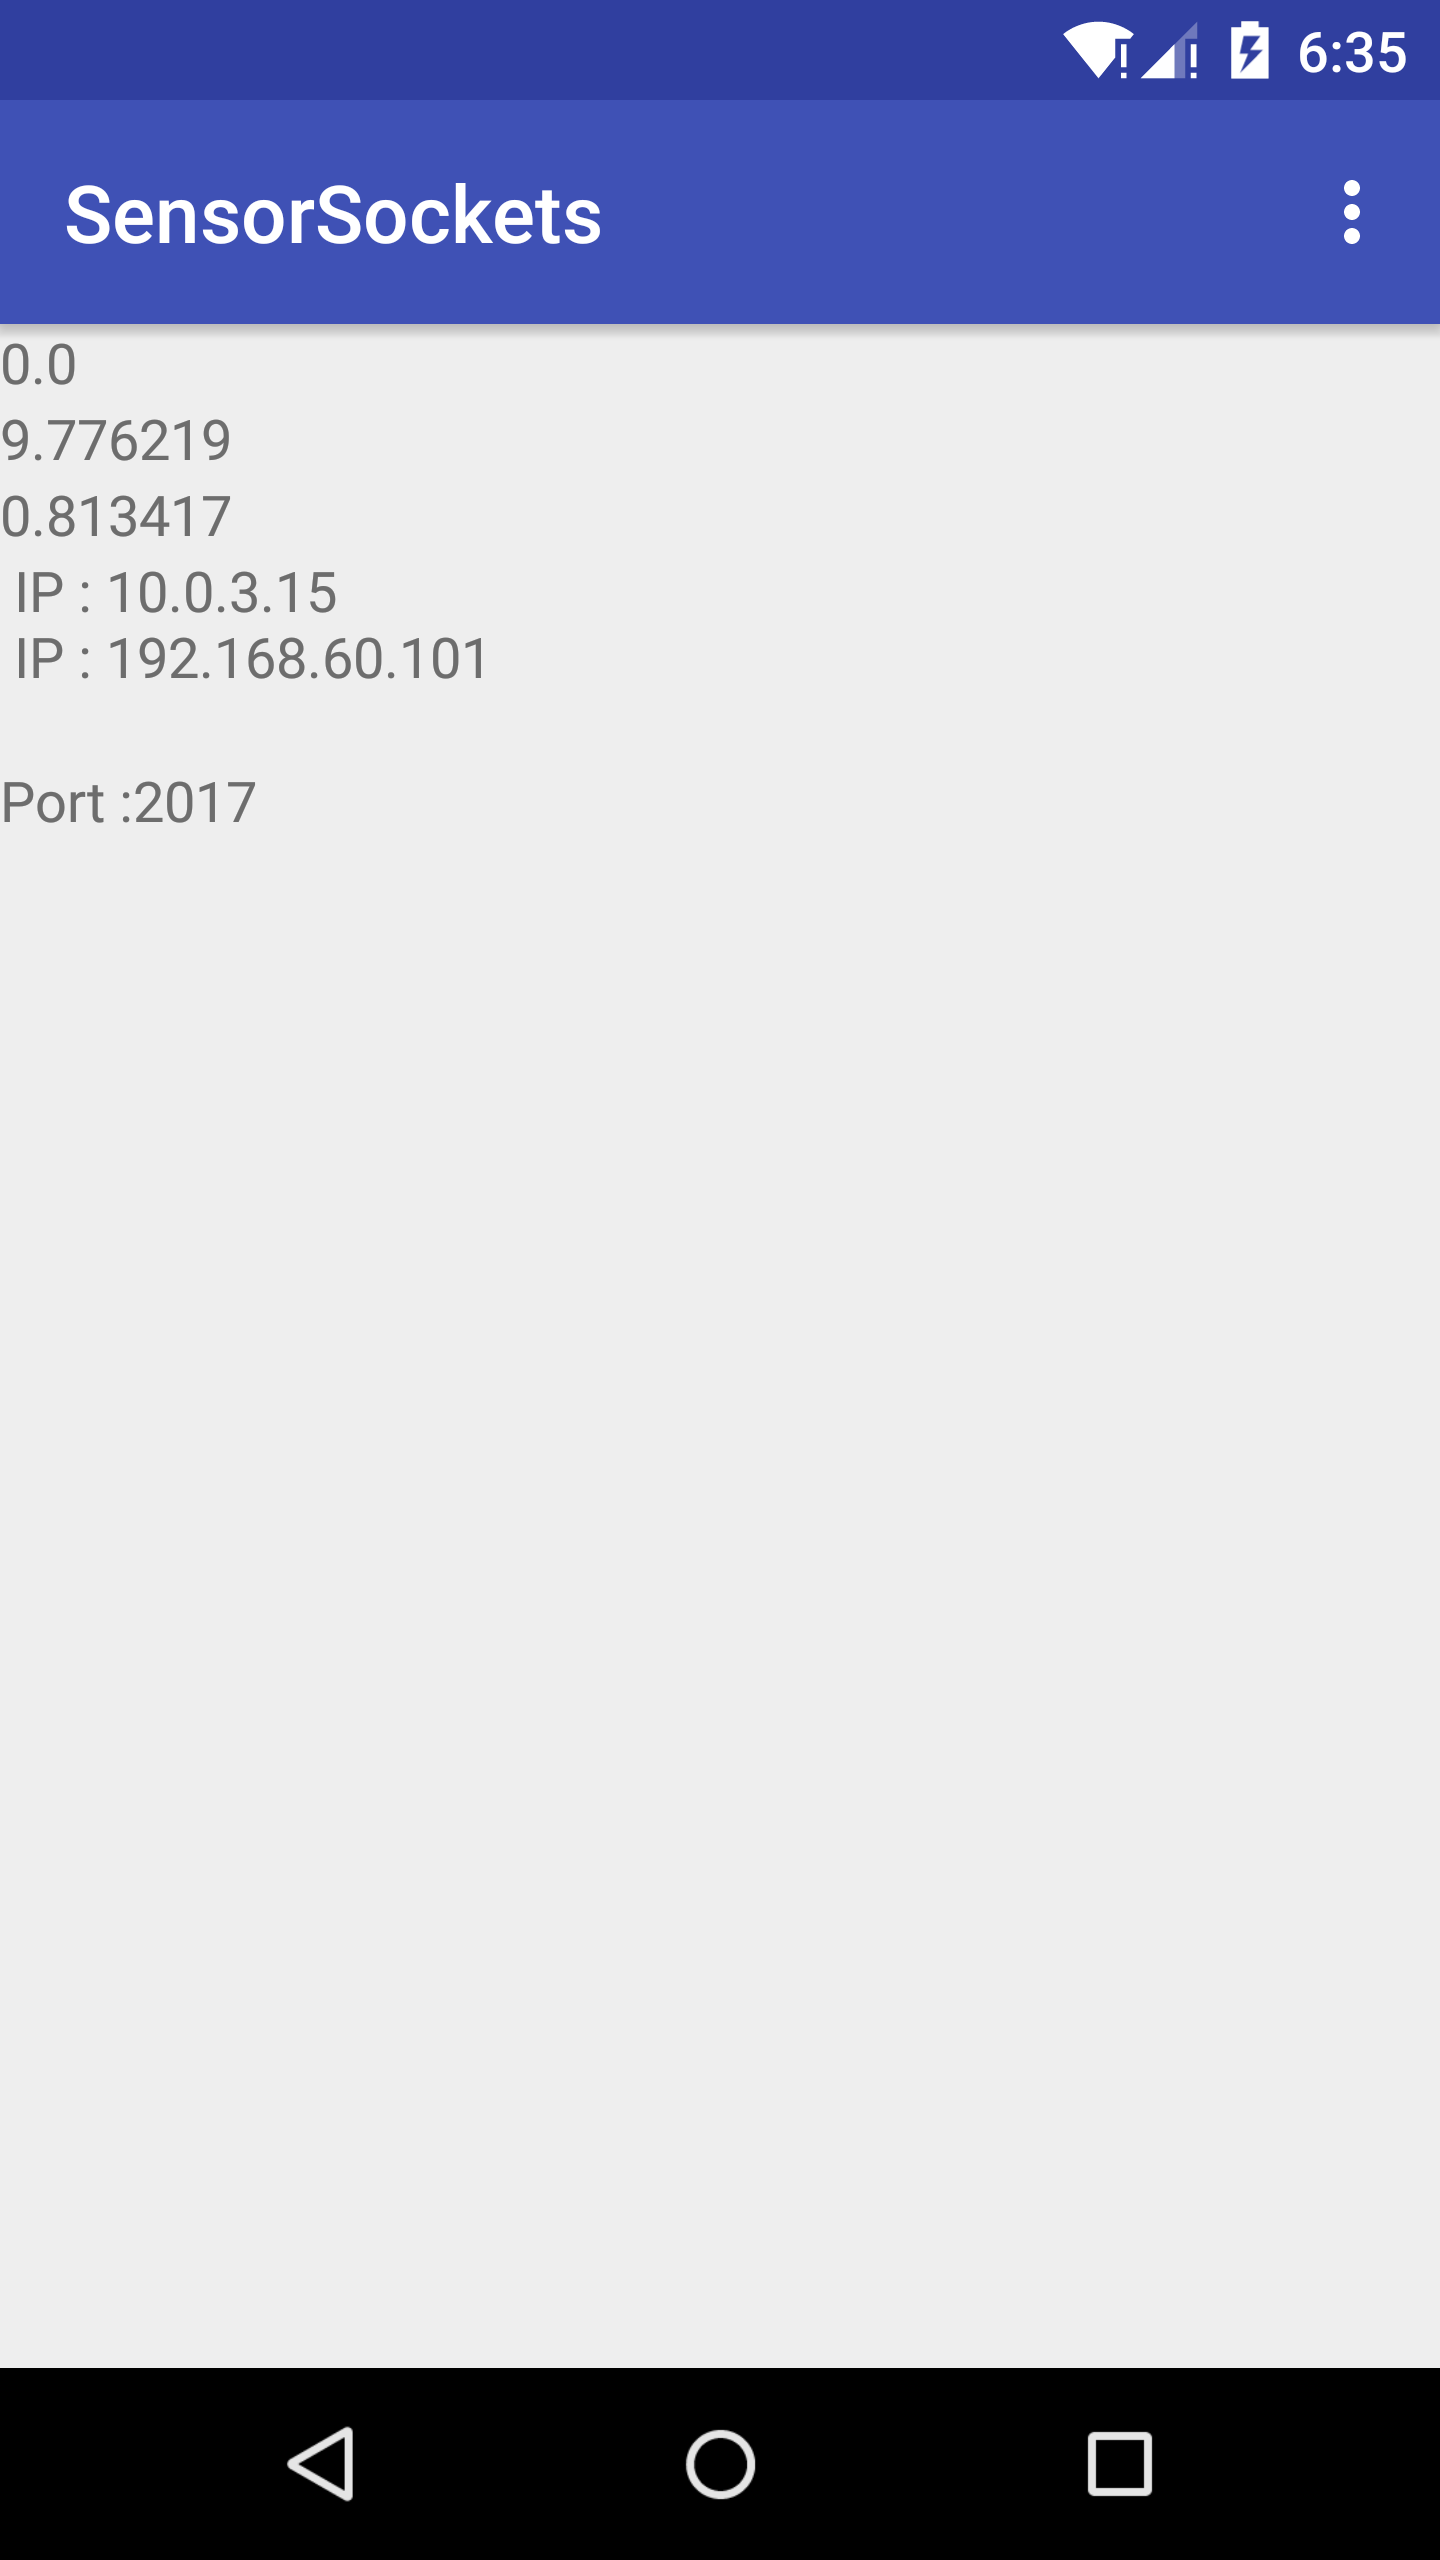
\includegraphics[width =.45\textwidth]{App1}\quad
    	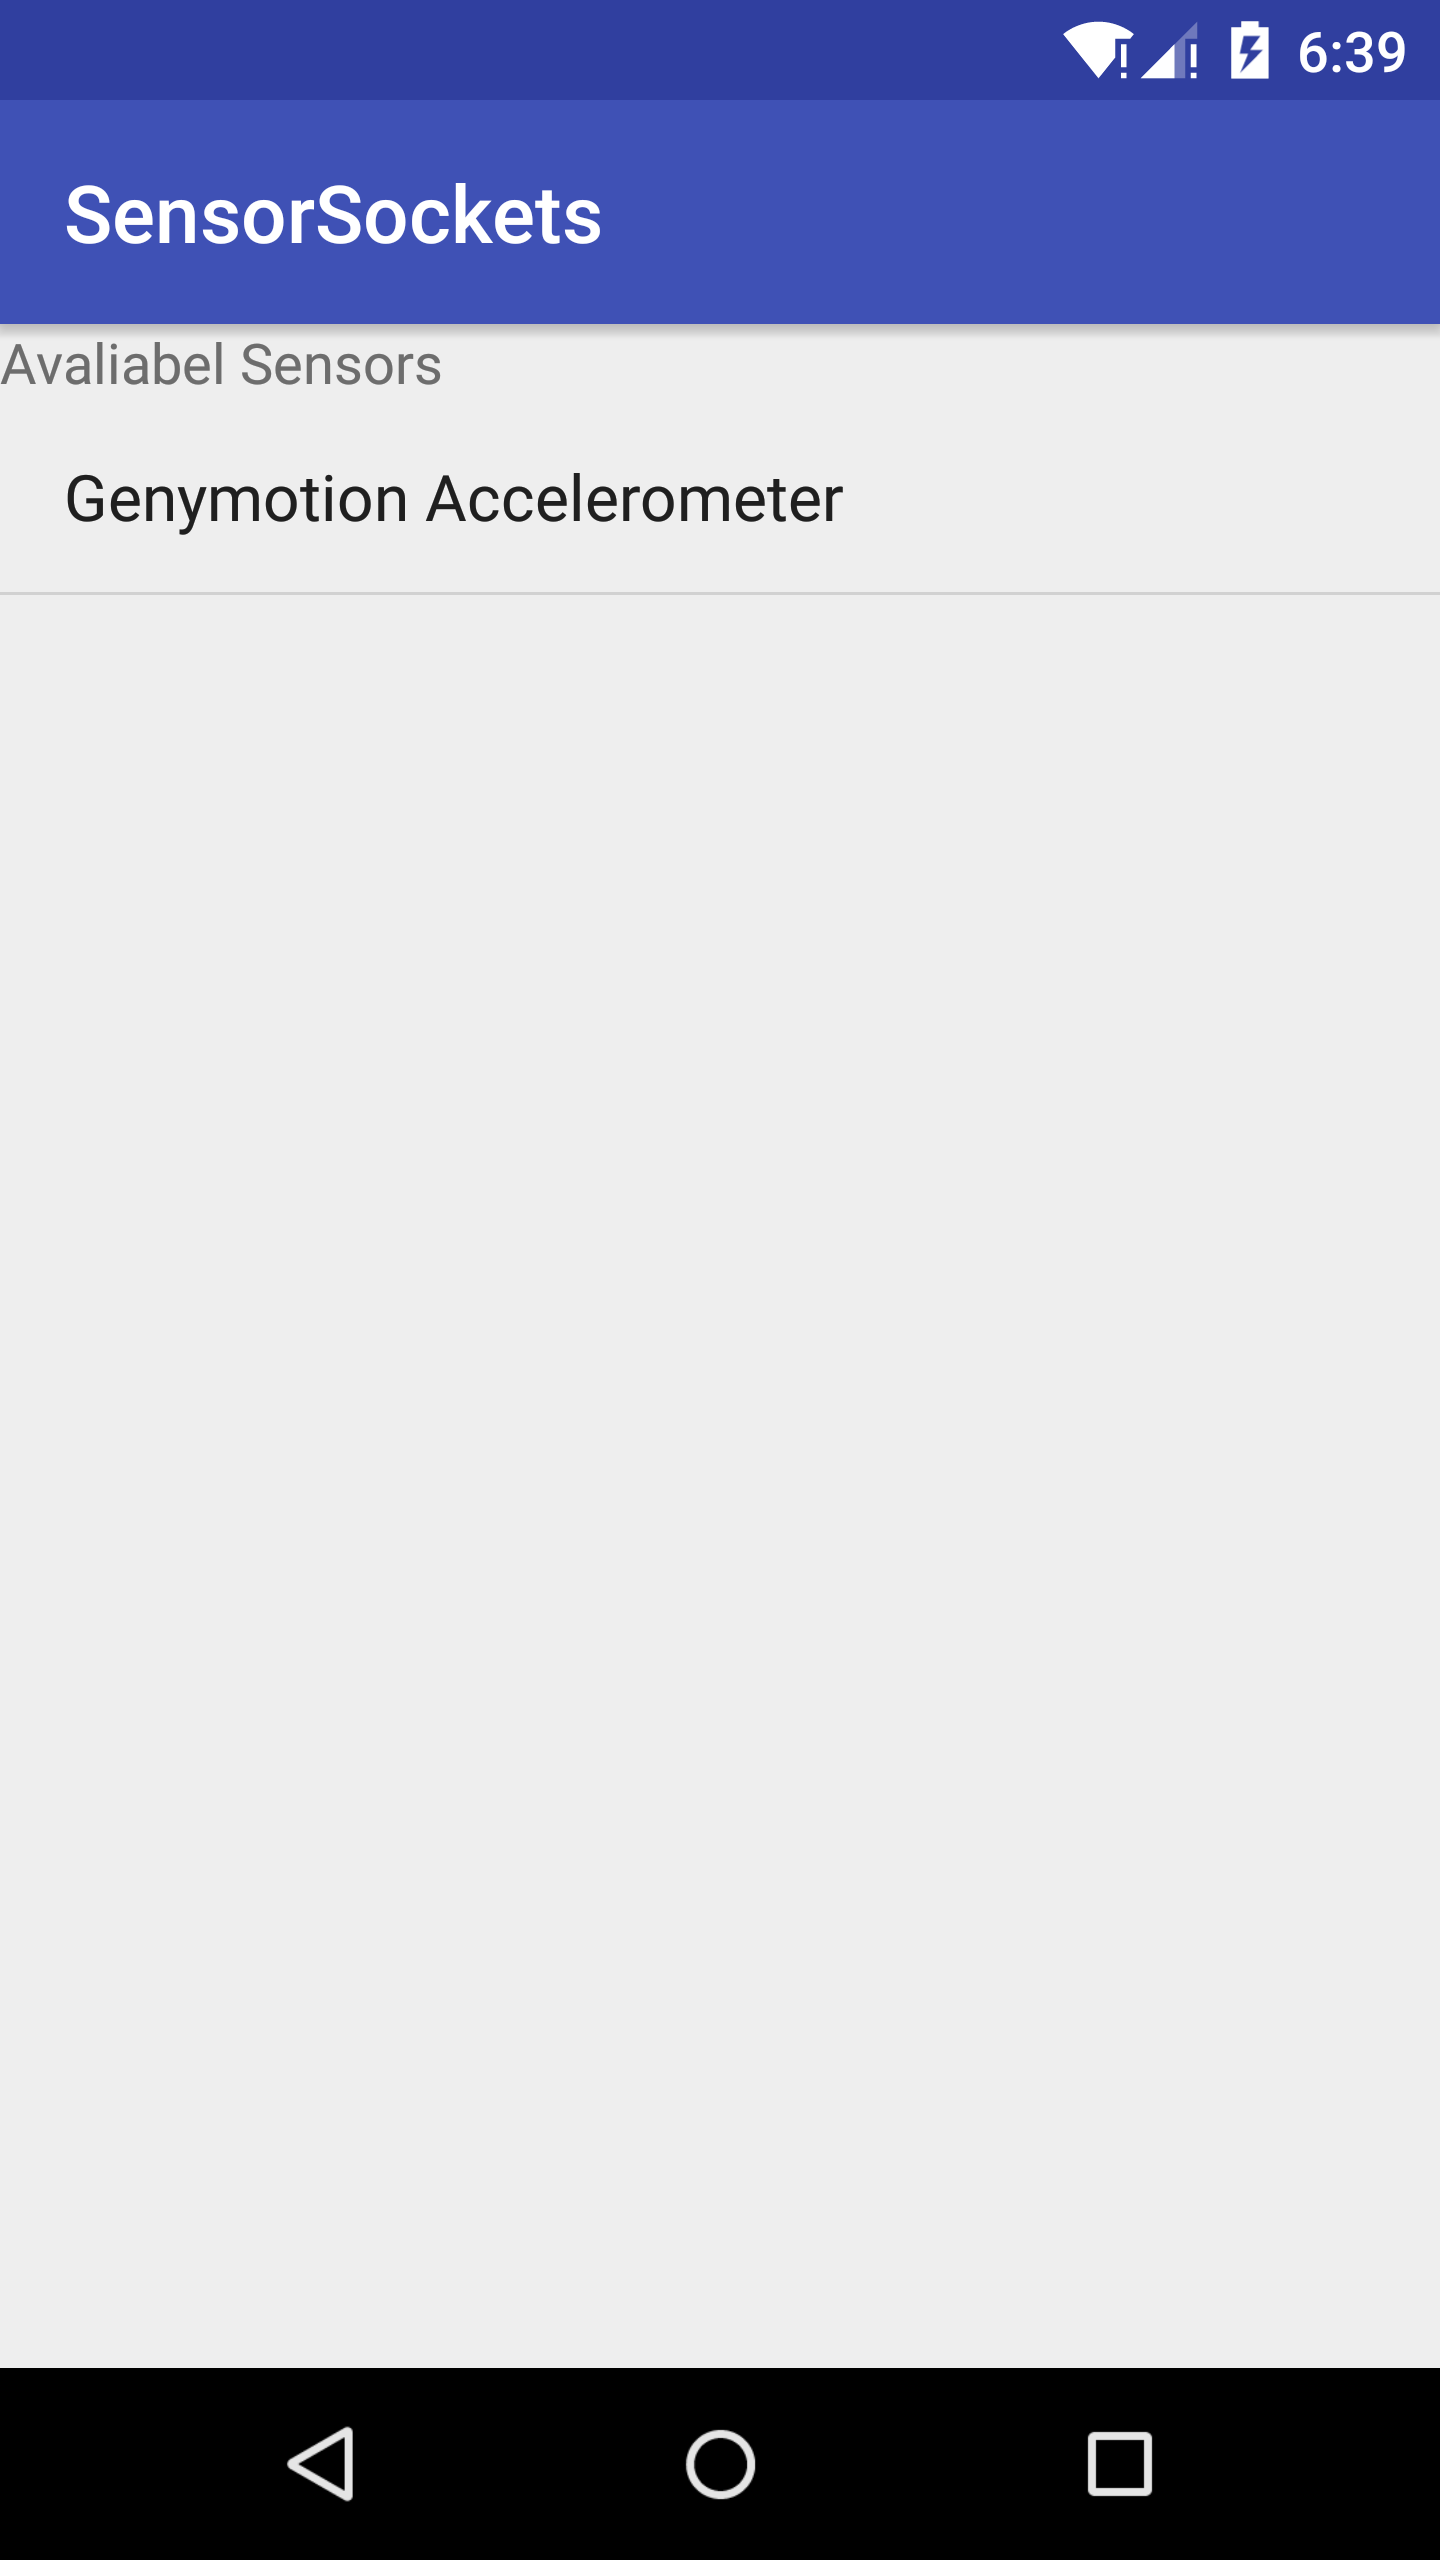
\includegraphics[width =.45\textwidth]{App2}
	\caption{Home page (left) and Sensor window (right)}
	\label{Fig:App1}
\end{figure}




\section{Communication Types}

	
	\subsection{Joystick}
	the wireless joystick communicates with the Raspberry Pi, using a ROS node called ‘joy’, and send a keystroke to it. Then the Raspberry Pi find the key pressed using a python library called ‘pygame’ and send a proper character on the serial port to the Arduino, our low-level interface with the servomotors. Lastly, the Arduino checks the received character and perform the needed action.
	\begin{figure}[h]		
		\centering
		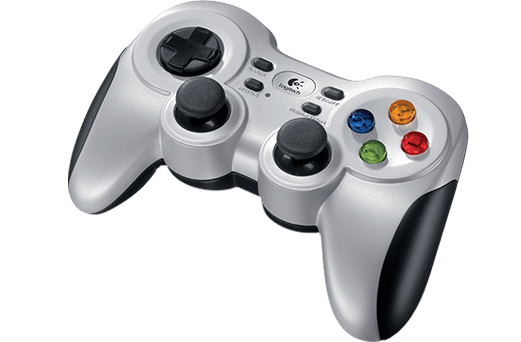
\includegraphics[width =.45\textwidth]{logitech_joy}
		\caption{JoyStick.}
		\label{Fig:joy}
	\end{figure}

	\subsection{BT Joystick}
	Goals:
		Using the Mobile  Bluetooth to control the robot as it contain joystick simulator to send the command to RPi, also this app capable to receive a video recorded form the Mobile on the robot as a background to the joystick so we can control every thing from one app and to see what the robot see.
		
	How it works:
		Using serial communication to Send data between two Bluetooth devices.
		\begin{figure}[h]		
			\centering
			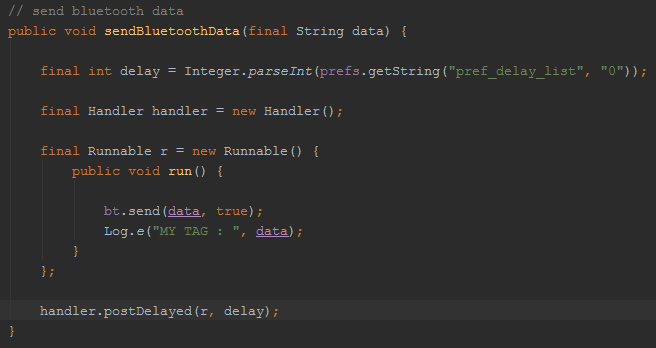
\includegraphics[width =.45\textwidth]{BT_app}
			\caption{Function for sending data through Bluetooth.}
			\label{Fig:BT}
		\end{figure}
		
		First we get the delay value from the setting the user saved.
		We make a handler that schedule the runnable to be executed at some point in the future.
		A new thread is made to send the Bluetooth data called "r" that will use the "bt" model that knows how to deal with Bluetooth then we tell the model to send the data.
		Then the handler will tell the runnable "r" to be executed at some point of the future that time will be determined by the variable "delay".
	How to use the program:
	\begin{itemize}
		\item After opening the program, the program will show you a button to open Bluetooth press "turn on" and confirm opening Bluetooth for your device.
		\item The first thing you need to do is setting and choosing IP and Port that you will connect to.
		\item Remove the port if you will connect to a global server or leave it and choose the right port to connect to in the case of local server.
		\item Now to return to the main activity press run at the bottom-center of the screen and the age is loaded at the background.
		\item Choose a Bluetooth a device to connect to.
		\item Change the joypad buttons look alike config to make ever button send the intended data.
		\item Now use the joypad buttons to control the robot.
	\end{itemize}
		
	\subsection{Wi-Fi}
		Another line of communication is between our control station and an Android smart phone mounted on the robot through a TCP/IP client server application.
		\begin{itemize}
			\item What is TCP/IP?\\
			When two computers follow the same protocols—the same set of rules—they can understand each other and exchange data. TCP/IP (Transmission Control Protocol/Internet Protocol) is the basic communication language or protocol of the Internet that use this concept to communicate through the internet and become standard terminology for referring to this suite of protocols.		
			TCP/IP architecture omits some features found under the OSI model, combines the features of some adjacent OSI layers and splits other layers apart. The 4-layer structure of TCP/IP is built as information is passed down from applications to the physical network layer. When data is sent, each layer treats all of the information it receives from the upper layer as data, adds control information (header) to the front of that data and then pass it to the lower layer. When data is received, the opposite procedure takes place as each layer processes and removes its header before passing the data to the upper layer. 
			
			- Application Layer\\
			The Application Layer in TCP/IP groups the functions of OSI Application, Presentation Layer and Session Layer. Therefore any process above the transport layer is called an Application in the TCP/IP architecture. In TCP/IP socket and port are used to describe the path over which applications communicate. Most application level protocols are associated with one or more port number.
			Transport Layer. In TCP/IP architecture, there are two Transport Layer protocols. The Transmission Control Protocol (TCP) guarantees information transmission. The User Datagram Protocol (UDP) transports datagram without end-to-end reliability checking. Both protocols are useful for different applications.
			
			- Network Layer\\
			The Internet Protocol (IP) is the primary protocol in the TCP/IP Network Layer. All upper and lower layer communications must travel through IP as they are passed through the TCP/IP protocol stack. In addition, there are many supporting protocols in the Network Layer, such as ICMP, to facilitate and manage the routing process.
			
			- Network Access Layer\\
			In the TCP/IP architecture, the Data Link Layer and Physical Layer are normally grouped together to become the Network Access layer. TCP/IP makes use of existing Data Link and Physical Layer tandards rather than defining its own. Many RFCs describe how IP utilizes and interfaces with the existing data link protocols such as Ethernet, Token Ring, FDDI, HSSI, and ATM. The physical layer, which defines the hardware communication properties, is not often directly interfaced with the TCP/IP protocols in the network layer and above. []
			
			\begin{figure}[H]		
				\centering
				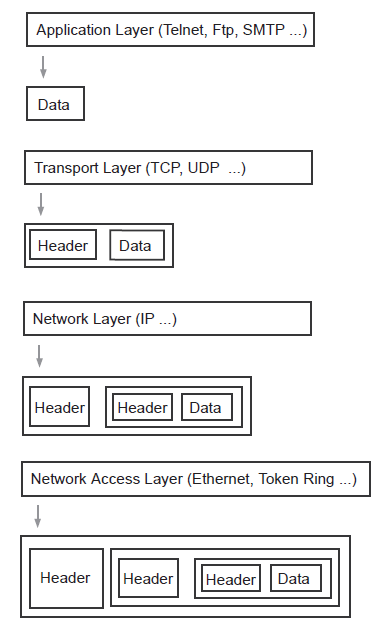
\includegraphics[width =.8\textwidth,height=16cm]{TCP_IP_Protocol_Stack_4_Layer_Model}
				\caption{TCP/IP Protocol.}
				\label{Fig:TCP/IP}
			\end{figure}
		
			TCP/IP uses the client/server model of communication in which a computer user (a client) requests and is provided a service (such as sending a Web page) by another computer (a server) in the network. TCP/IP communication is primarily point-to-point, meaning each communication is from one point (or host computer) in the network to another point or host computer. TCP/IP and the higher-level applications that use it are collectively said to be "stateless" because each client request is considered a new request unrelated to any previous one (unlike ordinary phone conversations that require a dedicated connection for the call duration). Being stateless frees network paths so that everyone can use them continuously. (Note that the TCP layer itself is not stateless as far as any one message is concerned. Its connection remains in place until all packets in a message have been received.)
			
			\item Protocol
			A protocol is the special set of rules that end points in a telecommunication connection use when they communicate. Protocols specify interactions between the communicating entities. 
			Protocols exist at several levels in a telecommunication connection. For example, there are protocols for the data interchange at the hardware device level and protocols for data interchange at the application program level. In the standard model known as Open Systems Interconnection (OSI), there are one or more protocols at each layer in the telecommunication exchange that both ends of the exchange must recognize and observe. Protocols are often described in an industry or international standard.
			
			The TCP/IP Internet protocols, a common example, consist of:
			Transmission Control Protocol (TCP), which uses a set of rules to exchange messages with other Internet points at the information packet level
			Internet Protocol (IP), which uses a set of rules to send and receive messages at the Internet address level
			Additional protocols that include the Hypertext Transfer Protocol (HTTP) and File Transfer Protocol (FTP), each with defined sets of rules to use with corresponding programs elsewhere on the Internet
			
			\item The Protocol Used In ZagHexa Robot
			
			Client will send "I" character in the first time of connection, Server will reply by an array of string in this format {"Sensor1\_name, ID, Sensor2\_name,ID, ..etc"}
			Ex:	{"gyroscope, 3, GPS, 4, ..etc"}
			
			Client will store this array into an text file to retrieve the ID for future requests.
			Client can do one of these requests :
			\begin{itemize}
				\item "A" character  to send all sensors data.
				\item ID number to select one sensor to get its data.
			\end{itemize}
				
			Server will reply in the first case by an array of numbers in the same order of the sensors in the index file, in the second case it will reply by a single float number that its index match the request one.\\\\\\
			
		\end{itemize}


\section{Sonar System}
\subsection{Main Components}
	\begin{enumerate}
		\item Ultrasonic sensor
			\begin{figure}[H]
				\centering
				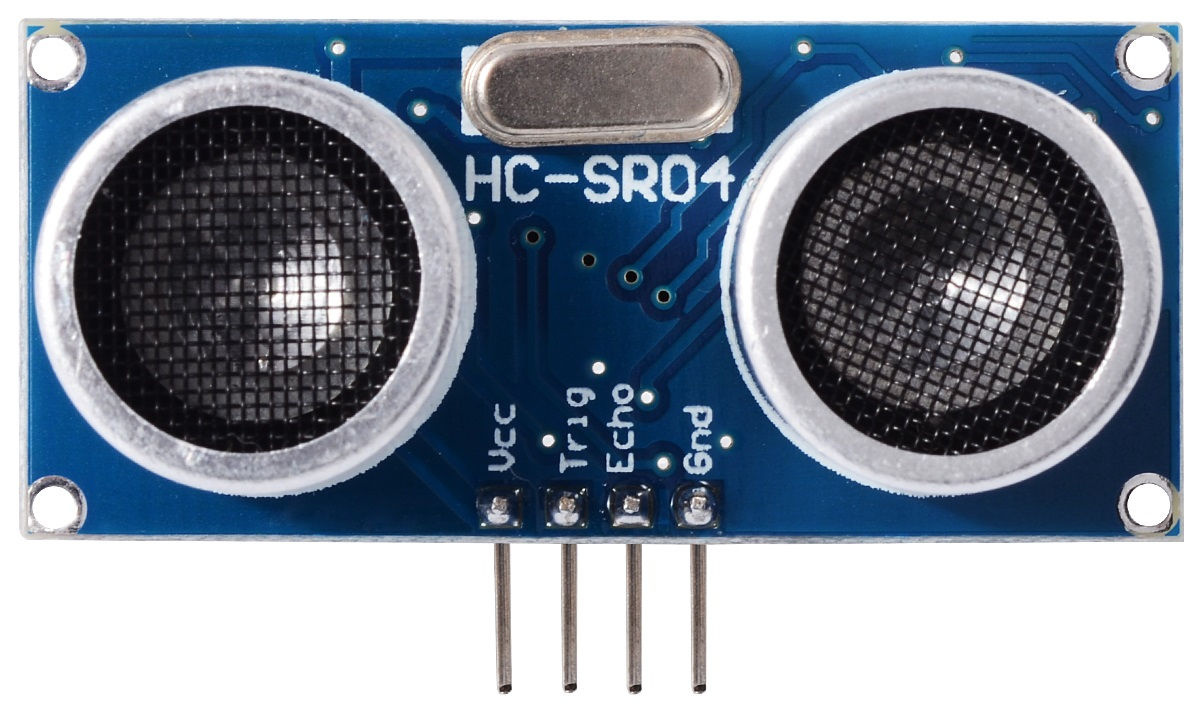
\includegraphics[width=10cm,height=5cm]{figures/ultra}
				\caption{Ultrasonic sensor}
				\label{Fig:ultrasonic}
			\end{figure}
		An Ultrasonic sensor is a device that can measure the distance to an object by using sound waves. 
		It measures distance by sending out a sound wave at a specific frequency and listening for that sound wave to bounce back. 
		By recording the elapsed time between the sound wave being generated and the sound wave bouncing back, it is possible to calculate the distance between the sonar sensor and the object.
		Since it is known that sound travels through air at about 340 m/s you can take the time for the sound wave to return and multiply it by 340 meters to find the total round-trip distance of the sound wave. 
		Round-trip means that the sound wave traveled 2 times the distance to the object before it was detected by the sensor; it includes the 'trip' from the sonar sensor to the object AND the 'trip' from the object to the Ultrasonic sensor (after the sound wave bounced off the object).
		To find the distance to the object, simply divide the round-trip distance in half.
		\vspace{0mm}
		\begin{figure}[H]
			\centering
			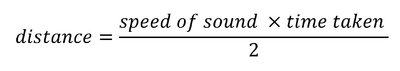
\includegraphics[width=10cm,height=2.5cm]{figures/ultra2}
			\caption{Distance calculation}
			\label{Fig:Distance calculation}
		\end{figure}
		\vspace{0mm}
		It is important to understand that some objects might not be detected by ultrasonic sensors. 
		This is because some objects are shaped or positioned in such a way that the sound wave bounces off the object, but are deflected away from the Ultrasonic sensor. 
		It is also possible for the object to be too small to reflect enough of the sound wave back to the sensor to be detected.
		Other objects can absorb the sound wave all together (cloth, carpeting, etc), which means that there is no way for the sensor to detect them accurately. 
		These are important factors to consider when designing and programming a robot using an ultrasonic sensor.
		
		\item PIR sensor
		 \vspace{0mm}
		 \begin{figure}[H]
		 	\centering
		 	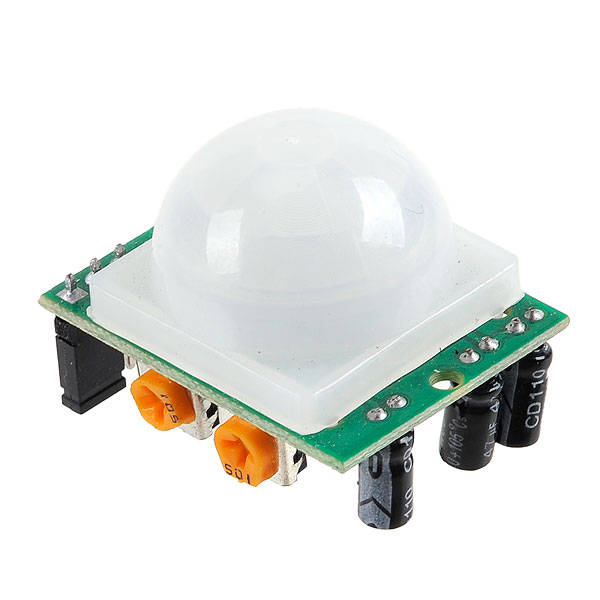
\includegraphics[width=7cm,height=4cm]{figures/PIR}
		 	\caption{PIR sensor}
		 	\label{Fig:PIR sensor}
		 \end{figure}
		 \vspace{0mm}
		 PIR sensors allow you to sense motion, almost always used to detect whether a human has moved in or out of the sensors range. 
		 They are small, inexpensive, low-power, easy to use and don't wear out easily.
		 For that reason they are commonly found in appliances and gadgets used in homes or businesses. 
		 \textbf{The working principle}: The module actually consists of a Pyroelectric sensor which generates energy when exposed to heat.
		 That means when a human or animal body will get in the range of the sensor it will detect a movement because the human or animal body emits heat energy in a form of infrared radiation. That’s where the name of the sensor comes from, a \textbf{Passive Infra-Red sensor}. And the term “passive” means that sensor \textbf{is not} using any energy for detecting purposes, it just works by detecting the energy given off by the other objects.
		 \vspace{0mm}
		 \begin{figure}[H]
		 	\centering
		 	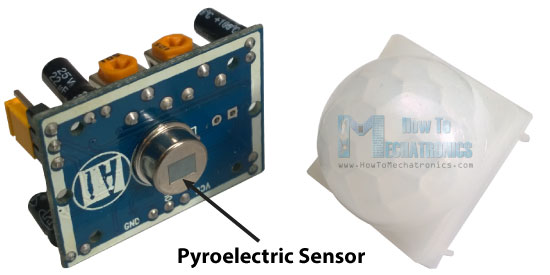
\includegraphics[width=10cm,height=5cm]{figures/PIR2}
		 	\caption{PIR sensor inside}
		 	\label{Fig:PIR sensor}
		 \end{figure}
		 \vspace{0mm}
		 The module also consists a specially designed cover named Fresnel lens, which focuses the infrared signals onto the pyroelectric sensor.
		  \vspace{0mm}
		 \begin{figure}[H]
		 	\centering
		 	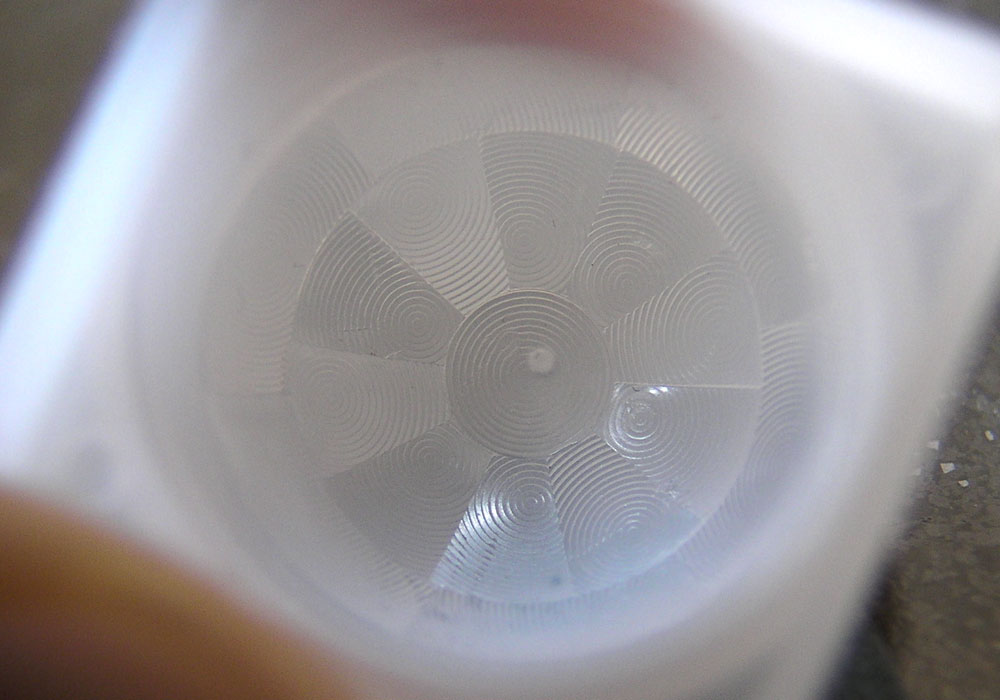
\includegraphics[width=14cm,height=14cm]{figures/PIR3}
		 	\caption{PIR sensor inside}
		 	\label{Fig:PIR sensor}
		 \end{figure}
		 \vspace{0mm}
		\item Servo motor 
		\item Arduino board and Jumper wires
	\end{enumerate}

\subsection{Circuit scheme}

\begin{figure}[H]
	\centering
	\includegraphics[width=14cm]{figures/sonar}
	\caption{Circuit scheme}
	\label{Fig:Scheme}
\end{figure}
The Ultrasonic Sensor is connected to the pins number 4 and 5, PIR to pin 7 and the servomotor to the pin number 6 on the Arduino Board. 

Now we need to make a code and upload it to the Arduino Board that will enable the interaction between the Arduino and the Processing IDE.

\textbf{Hints about processing:}

\begin{enumerate}
\item \textbf{ }The Processing Development Environment (PDE) makes it easy to write Processing programs. Programs are written in the text editor and started by pressing the run button. 

\item  In Processing, a computer program is called a sketch. Sketches are stored in the Sketchbook, which is a folder on your computer. Sketches can draw two- and three-dimensional graphics.

\item  Processing has different programming modes to make it possible to deploy sketches on different platforms and program in different ways. The Java mode is the default. Other programming modes may be downloaded by selecting "Add Mode''.
\end{enumerate}

The Target is to make the calculation of distance, moving servo and publishing angle and PIR give the signal if it detected something to the serial port.

So as processing can handle and read their values and process them to get the output.

This is simply demonstrated in this figure:

\begin{figure}[H]
	\centering
	\includegraphics[width=14cm,height=7cm]{figures/sonar2}
\end{figure}
After uploading the code to Arduino and checked that the output on serial with the required pattern.

Now we will receive the values for the angle and the distance measured by the sensor from the Arduino Board into the Processing IDE using the SerialEvent() function which reads the data from the Serial Port and we will put the values of the PIR, angle and the distance into the variables myPIR, myAngle and myDistance.

These variables will be used for drawing the sonar, the lines, the detected objects{\dots}etc.

For drawing the sonar main screen, this function~was made \textbf{drawRadar()}~which consist of~\textbf{arc()}~and~\textbf{line()} functions as you see in the next figure.
They are 4 half circles and lines to demonstrate the degrees meter.
\begin{figure}[H]
	\centering
	\includegraphics[width=14cm,height=7cm]{figures/sonar3}
\end{figure}
For drawing the line that is moving along the radar this function \textbf{drawLine(). }Its center of rotation is set with the \textbf{translate() }function and using the line() function in which the myAngle variable is used the line is redrawn for each degree.
\begin{figure}[H]
	\centering
	\includegraphics[width=14cm,height=7cm]{figures/sonar4}
\end{figure}
 For drawing the detected objects this function \textbf{drawObject()} gets the distance from ultrasonic sensor, transforms it into pixels and in combination with the angle of the sensor draws the object on the sonar.
\begin{figure}[H]
	\centering
	\includegraphics[width=14cm,height=7cm]{figures/sonar5}
\end{figure}

For the text on the screen the function \textbf{drawText()} draws texts on particular locations. All of these functions are called in the main \textbf{draw()} function which repeats all the time and draws the screen. 

And the final output as you can see 
\begin{figure}[H]
	\centering
	\includegraphics[width=14cm,height=8cm]{figures/sonar6}
\end{figure}

\section{GUI}

Future work

%%%%%%%%%%%%%%%%%%%%%%%%%%%%%%%%%%%%%%%%%%%%%%%%%%%%%%%%%%%%%%%%%%%%%%%%%%%%%%%
\setchapterpreamble[o]{%
    \dictum[Alan Turing, \textit{(British pioneering computer scientist, cryptanalyst,$\cdots$, and philosopher, 1912--1954)}]{%
        ``A computer would deserve to be called intelligent if it could deceive a human into believing that it was human.''}}

\chapter{Mechanical Design} \label{ch:mechanical}
%!TEX root = finalReport.tex
%!TEX encoding = UTF-8 Unicode
%==============================================================================

\section{Design Characteristics}
In the following section, the main design characteristics and modeling issues are discussed in order to show how the proposed design procedure can be implemented. It is worth mentioning also that other design characteristics exist and additional features can be considered for specific applications. Thus, the most remarkable design characteristics have been considered as examples for filling in the data in the cause and effect matrix.

\subsection{Robot Body Architecture}
There are two basic architectures of hexapod robots: rectangular and hexagonal as shown in \ref {figure a.png}. The first one has six legs distributed symmetrically along two sides,each side having three legs. The second haslegs distributed axi-symmetrically around the body, in a hexagonal or circular shape.

\begin{figure}[h]
	\centering
	\includegraphics{figure_a}
	\caption{Basic architectures of hexapod robots}
	\label{figure a.png}
\end{figure}

Many references can be found in the literature on rectangular six-legged robots, they describe the longitudinal stability margin for rectangular hexapods. Also, the feasible walking gaits have been widely investigated and tested. Bilateral symmetry may be better suited than radial symmetry to move along a straight line. Rectangular architectures require a special gait for turning action; generally, they need four steps in order to realize a turning action. Hexagonal hexapod robots demonstrate better performances than rectangular robots for some aspects. As example hexagonal robots can have many kinds of gaits and can easily change direction—in fact true radial symmetry implies that all legs are equal and the body has no “front” or “rear”—there is thus no preferential directionfor the motion. It is proved that hexagonal hexapods can easily steerin all directions and that they have a longer stability margin. It isfound that hexagonal robots rotate and move in all directions at the same time,better than rectangular ones, by comparing stability margin and stroke in wave gait.It is proved theoretically that hexagonal hexapod robots have superior stability margin,stride and turning ability compared to rectangular robots.

\subsection{Kinematic Architectures of Legs}
Kinematics architecture depends on the factors related to the application in which the hexapod robot is required for, as for example the terrain form, the workspace and the payload. Literature shows that there is a number of different leg types currently employed for hexapod walking robots. All have advantages and disadvantages. \ref{figure b.png} shows a schematic classification of hexapod legs types.

\begin{figure}[h]
	\centering
	\includegraphics[width =0.85\textwidth]{figure_b}
	\caption{Classification of hexapod leg types}
	\label{figure b.png}
\end{figure}

At the first stage, one can choose between bio inspired and non-zoomorphic legs. Bio inspired leg configuration is motivated primarily by animal gait, such as reptiles, mammals or arachnid. The first one has legs and bodies for moving over rough and uneven terrains. The principal characteristic of the Reptilian type is that the legs are placed on both ends of the protruding body and knees to the side of the base. Mammals’ bodies are above the legs, which gives less support to the base and lower power consumption is needed to support the body, but it requires more stability than other types of animal. In Arachnid configuration, legs extremities are situated on both sides, sticking the knees at the top of the spider’s body. The orientation of the legs in respect to the body of the hexapod robot can be done with three configurations: frontal, sagittal or circular as shown in \ref{figure c.png}.
\begin{figure}[h]
	\centering
	\includegraphics[width =0.75\textwidth]{figure_c}
	\caption{Hexapod leg configurations}
	\label{figure c.png}
\end{figure}

In the first one, the directions are perpendicular to the advancement of the legs’ position, unlike the sagittal, which moves parallel to the robot legs, while in the circular arrangement the legs are positioned radially to the body of the system allowing the mechanism to move in any direction. In the mammalian configuration, the legs are below the body and can place the knees in different positions depending on the application it requires, shown in figure (d). Non zoomorphic legs can be hybrids, telescopic or under-actuated, a solution named Roller-Walker is presented. The principle through which the robot propels itself during wheeled locomotion is the same as that of the skaters.

\begin{figure}[h]
	\centering
	\includegraphics[width =0.75\textwidth]{figure_d}
	\caption{Joint configurations}
	\label{figure d.png}
\end{figure}

\subsection{Actuator Types}
Many kinds of actuators can be employed for operating hexapod walking robots. The majority of hexapods is actuated by electric rotating motors (Servo motors), as they are relatively cheap, easy to control and there are suitable technologies to store the energy.\\ 
Linear motors are able to generate considerable forces at very considerable speeds. However, these do not yet appear to have been utilized in many hexapods since they have a limited movable range to weight ratio. Pneumatics actuators have very low stiffness, inaccurate response, and low power to weight ratio. Pneumatics actuators, or air muscle, are able to offer a fast response time but they need an on-board air supply as bottles or compressors that are heavy pieces of equipment. Hydraulics actuators have high power/weight ratio; they are able to supply very high force, but suffer from the serious drawback of having to carry an engine to drive the pump. Hydraulics actuators are suitable for larger sized hexapod robots.\\
Unconventional actuators for hexapod robots can also be materials that can change shape through the direct application of electricity or a chemical agent. Ionic polymer-metal composites, for example, are materials that exhibit high strains under applied voltage differences allowing them to change from a sheet shape into curved shapes. Polyacrylonitrile is a form of artificial silk, classed as a gel polymer. It can respond fast, but the activation method is a change in pH, which requires the fibers to be housed in a watertight bag. Another class of materials that can change shape under the application of electricity is the Shape Memory Alloys (SMA), such as a nickel-titanium alloy that exhibits extreme contraction when heated.\\
Contraction rates are controlled by the heating and cooling; the major drawback resulting in slow response times and small operating forces. Thus, despite a great research interest and the building of some prototypes, the uses of SMA as hexapod actuators have been very limited. Present trends indicate that they are more suited to micro robots.

\subsection{Actuators Arrangements}
Typically, specific actuator arrangements are developed in order to obtain maximum leg workspace with a minimal kinematic structure. Several types of geometrical arrangements such as in \ref{figure_e} are recurrent in literature.
\begin{figure}[h]
	\centering
	\includegraphics[width =0.5\textwidth]{figure_e}
	\caption{Three DoF solution}
	\label{figure_e}
\end{figure}

The design consists of links connected through knee joints. The walking motion is accomplished by controlling the angle of the links to position the feet. There are a number of different ways in which the joints can be actuated. Options include mounting the motor at the joint itself, or using a pulley and belt or lead screw \ref{figure_f} to set the angle of the knee using an actuator mounted near the base of the leg.
\begin{figure}[h]
	\centering
	\includegraphics{figure_f}\qquad
    	\includegraphics{figure_g}
	\caption{Pinion-belt arrangement (left) and Lead screw leg (right)}
	\label{figure_f}
\end{figure}


The major drawback of last design is the necessity to actuate remote joints. On the other hand, latching the actuator at the knee joint adds various dynamic effects to the leg which have to be compensated by the controller. This adds complexity to the control algorithms needed to move the leg.\\
It also requires more powerful motors at the hip joint to move the added mass of the leg. Remote actuation, in which the actuators are located at the base of the leg, eliminates some of these problems, at the cost of increasing the complexity of the mechanism. The coupling of the motion of the end effector relative to the actuators is another undesirable characteristic of this leg design.  Another potential leg design is modeled according to a typical mammalian leg with a four-bar linkage structure. The major drawback of this design is that the motions are highly coupled and the effective workspace is somewhat limited. Moreover, the entire weight of the robot is supported by the hip joint and they necessitate a powerful and expensive motor.

\section{Walking Gaits}
A gait is a sequence of leg motions coordinated with a sequence of body motions for moving the overall body of the robot in the desired direction and for orientation from one place to another. A gait is described as periodic when similar states of the same leg during successive strokes occur at the same interval for all legs. Periodic gaits are suitable for smooth terrain and they have been studied by several investigators. Figure 9 shows the scheme of some periodical hexapod gaits; white color indicates that the foot is in ground contact and the black color otherwise. Figure 9a reports the hexapod legs’ description.

\subsection{Tripod gait}
Tripod gait is a regular, periodic gait where the anterior and posterior legs on one side lift in time with the contralateral middle leg, forming alternating tripods. Thus, it is based on two groups of legs. During each step the first group of the legs is lifted and is rotated forward and is laid upon on the ground. Then the other group is lifted. Now both groups are moving, the first group backward, the second group forward and finally the second group is laid on the ground. It is obvious that both groups perform the same movement, but they are shifted by half a period. Tripod gait is very fast, but also very unstable. That is because at one moment half of the whole weight of the robot is only on one leg, which can lead to slip or even to fall. This is a gait suitable for high speed walking over relatively flat ground.

\subsection{Wave Gait}
Another gait is wave, which is the most stable gait, but also the slowest. Wave gait consists of a sequential adjustment of legs forward and only when all the legs are set to the new positions, the step is completed. In each phase of step maximally one leg is lifted up, which leads to high stability of this gait.

\subsection{Ripple Gait}
Ripple gait is inspired by insects. Each leg performs the same move – up, forward, down, backward.

\begin{figure}[h]
	\centering
	\includegraphics[width =0.8\textwidth]{figure_h}
	\caption{Gait diagram of hexapodal gaits}
	\label{figure h.png}
\end{figure}

\ref{figure h.png} shows the movement of each leg in time. A high value represents leg movement and low values means no movement. Tripod, wave and ripple gaits are shown in this figure. Tripod has two group of legs, all the legs in the same group move at once. In the wave gait only one leg is moving at any time. After all legs are set up to their new positions, step is completed. In the ripple gait all legs move the same way, but their moves are shifted. Leg moves partially overlap. In other words, the time when the first foot is lifted and begins to move forward, the second leg begins to lift up. In this way the robot cycles through all legs.

These are the most common gaits. Theoretical number of different gaits N can be calculated using equation: N = (2K - 1)!, where K is the number of the legs of the robot. Not all of them are usable for effective locomotion. For hexapod robot it is 11! = 39 916 800 possibilities of locomotion. The number is quite large, because this equation calculates all possible motions, like motion up and down, which of course doesn’t lead to an effective movement.

\section{Robot Kinematics}

\subsection{Robot body frame}
The origin of the robot base frame will be in the center of the body, structured with Z-axis pointing up, the X-axis positioning right and Y-axis pointing forwards with respect to the robot front side as depicted in \ref{Loc}.

\begin{figure}[h]
	\centering
	\includegraphics[width =0.8\textwidth]{Fig3}
	\caption{ Location of body frame relative to robot hardware.}
	\label{Loc}
\end{figure}

\subsection{Leg frames and notations}
The design of hexapod constitutes the kinematic configuration of a hexapod robot, with each leg acting as an independent serial manipulator with three degrees of freedom. Figure \ref{fig1} shows the actual prototype of our robot.

\begin{figure}[h]
	\centering
	\includegraphics[width =.8\textwidth]{fream}
	\caption{  Final leg design (top right) and its notations, reference frames, joints and links.}
	\label{fream}
\end{figure}

The final leg design and its links and joints notations are given in \ref{fream}. The robot leg is made of links and joints as noted on \ref{leg}, different links of robot leg are called Femur, Tibia and Tarsus. As depicted in figure, the robot leg frame starts with link 0, which is the point where the leg is attached to the body, link 1, is Femur, link 2 is the Tibia and link 3 is Tarsus. The joints are located at the inner end of their respective link. Frames are attached to outer end of their respective links, this means that joint 2 rotates about the Z-axis of frame 1.

\begin{figure}[h]
	\centering
	\includegraphics[width =.8\textwidth]{Fig7}
	\caption{  Final leg design (top right) and its notations, reference frames, joints and links.}
	\label{leg}
\end{figure}

\subsection{Robot Leg Parameters}
Following the well-known Denavit-Hartenberg (DH) notation, coordinate frames for the robot leg are assigned. The assigned frames are shown in \ref{leg}. In figure, the body {b} and the zeroth {0} reference frames are attached to the stationary robot body. Therefore, they can be both considered as inertial frames. The axes of the body frame are arranged to be in accord with the actual robot-body orientation. The DH link parameters based on \ref{leg} are given in Table II.\\

The resulting homogeneous transformation matrices between the body and the zeroth frame and between the sequential link frames are given in (1).  In the formulas, the variables represented by $a$ stand for the length of the $i^{th}$ link (namely, the length of the portion of the link between the origins of $(i-1) th and i^{th}$ reference frames). The variables represented by $\theta_{ij}$ mean the sum of the $i^{th}$ and $j^{th}$ joint angles $(\theta_{ij}=\theta_i+\theta_j)$. C and S are for cos(.) and sin(.) functions, respectively.  The exact values of these variables corresponding to ZagHexa robot are: 
$\psi = 45^\circ, a_1= 5cm, a_2= 9cm, a_3= 18cm$
\begin{center}
\begin{tabular}{|c||c|c|c|c|}
	\hline
	Joint & $\theta_i$ & $\alpha_i$ & $a_i$ & $d_i$ \\ \hline
	1&		$\theta_1$ & $\pi/2$	& $a_1$ & 0 \\ \hline
	2&		$A_2$ & 0			& $a_2$ & 0 \\ \hline
	3&		$B_1$ & 0			& $a_3$ & 0 \\ \hline
\end{tabular}
\end{center}

Homogeneous matrices are used in derivation of positional relations between the successive frames.  In (3) the leg tip point position with respect to the body frame is given. The rotation matrices between the frames are given in (2). These rotation matrices are used in vector equations, especially while deriving the dynamic equations.
\begin{center}

\[
H^{(b,0)}=
\begin{bmatrix}
0 & \cos(\psi) & \sin(\psi) & 0 \\
-1&		0	   & 		0 	& 0\\
0 & -\sin(\psi)& \cos(\psi) & 0 \\
0 &		0	   & 		0 	& 1
\end{bmatrix}
\]
\end{center}

\begin{equation}
H^{(K-1,K)} =
\begin{bmatrix}
\cos\theta_k &-\cos\alpha_k\sin\theta_k &\sin\alpha_k\sin\theta_k &a_k\cos\theta_k\\
\sin\theta_k &\cos\alpha_k\cos\theta_k &-\sin\alpha_k\cos\theta_k &a_k\sin\theta_k\\
0 &\sin\alpha_k &\cos\alpha_k &d_k \\ 
0 &0 &0 &1
\end{bmatrix}
\end{equation}

\begin{align*}
H^{(0,3)} = H^{(0,1)} H^{(1,2)} H^{(2,3)} H^{(b,3)}= H^{(b,0)} H^{(0,3)}
\end{align*}

\begin{center}
	
	\[
	C^{(b,0)}=
	\begin{bmatrix}
	0 & \cos(\psi) & \sin(\psi) \\
	-1&		0	   & 		0 	\\
	0 & -\sin(\psi)& \cos(\psi) \\

	\end{bmatrix}
	\]
\end{center}

\begin{equation}
C^{(K-1,K)} =
\begin{bmatrix}
\cos\theta_k &-\cos\alpha_k\sin\theta_k &\sin\alpha_k\sin\theta_k \\
\sin\theta_k &\cos\alpha_k\cos\theta_k &-\sin\alpha_k\cos\theta_k \\
0 &\sin\alpha_k &\cos\alpha_k \\ 
\end{bmatrix}
\end{equation}
\begin{equation}
P_e^{(K-1,K)} (\theta) =
\begin{bmatrix}
C\psi(a_1S\theta_1+a_2S\theta_1C\theta_2+a_3S\theta_1C\theta{23})+S\psi(a_2S\theta_2+a_3\theta_{23}) \\
-(a_1C\theta_1+a_2C\theta_1C\theta_2+a_3C\theta_1C\theta_{23})  \\
-S\psi(a_1S\theta_1+a_2S\theta_1C\theta_2+a_3S\theta_1C\theta{23})+C\psi(a_2S\theta_2+a_3\theta_{23}) \\
\end{bmatrix}
\end{equation}
To derive the dynamic equations, first the inertia matrices of the links should be determined. Since the $k^{th}$ reference frame is stationary with respect to the $k^{th}$ link, the inertia tensor of the $k^{th}$ link around its center of mass appears to be a constant matrix with respect to the $k^{th}$ reference frame, as in (4). The values used in these formulations belong to the Hexapod robot. The resulting matrices for each link are in the form of (5).
\begin{equation}
\{J_K\}^{(K)} = J_K^{(K)} = J_K
\end{equation}
\begin{equation}
J_K = \begin{bmatrix}
J_{K1} & 0      & 0 \\
0      & J_{K2} & 0 	\\
0      & 0      & J_{K3} 
\end{bmatrix}
\end{equation}

\subsection{Inverse kinematics}
The forward kinematics (FK) is a simple equation used to calculate the position of the end effectors for the leg in the robot base frame, by injecting values of each joint angle. But the reverse operation, namely inverse kinematics (IK), is more complex. IK is employed to find all the joint angles given the position of the end effectors. In general, solving the IK equations can be a bit of a challenge. Some positions cannot be reached at all, as the physical system is unable to get there, and some end effectors positions can have more than one solution, and not all of them are desirable.
\begin{figure}[h]
    \centering
    \includegraphics[width =.55\textwidth]{Fig8.png}
    \caption{ Illustration of the 2D triangle with vertices in the coxa, the femur, and tibia link from origin.}
    \label{fig8}
\end{figure}
We solve the IK problem for each leg separately, as this makes it possible to solve it geometrically, by setting up some constrains. The first constraint for solving the IK equations due the fact that all robot joints allow rotation about one axis only. The second constraint is that the Femur, Tibia joints always rotate on parallel axes. The third set of constraints arises from the physical limitations for each joint, giving us some angular interval for each joint in which the servos can actually rotate the link. In \ref{leg}, the angles of movement are shown.
First, the coxa angle can be found directly by knowing the end effectors position then simply using $atan2(y,x)$ to calculate it.  \ref{eq:invS} through \ref{eq:invE} are used to find the individual joint angles.
\begin{align}
    \frac{x}{y} & =\tan (\gamma)\to \gamma =\tan ^{-1}\frac{x}{y} \label{eq:invS}\\
    L              & = \sqrt{Z_{offset}^{2}+(L_{1}+\cos (A_1 + A_2))^{2}}\\
    A_{1}        & = \cos ^{-1}(\frac{Z_{offset}}{L})\\
    Tibia^{2}  & =Femar^{2}+L^{2}-2(Femar)(L)\cos \alpha _{2} \\
    A_{2} & =\cos^{-1}(\frac{Tibia^{2}-Femar^{2}-L^{2}}{-2(Femar)(L)}) \\
    A & =A_{1} + A_{2}\\
    A & = \cos ^{-1}\left(\frac{Z_{offset}}{L})+\cos ^{-1}(\frac{Tibia^{2}-Femar^{2}-L^{2}}{-2(Femar)(L)}\right) \\
    B & = \cos^{-1}\left(\frac{L^{2}-Femar^{2}-Tibia^{2}}{-2(Femar)(Tibia)}\right) \label{eq:invE}
\end{align}
%%%%%%%%%%%%%%%%%%%%%%%%%%%%%%%%%%%%%%%%%%%%%%%%%%%%%%%%%%%%%%%%%%%%%%%%%%%%%%%

\setchapterpreamble[o]{%
	\dictum[Richard P. Feynman, \textit{(American theoretical physicist, 1918--1988)}]{%
		``It doesn't matter how beautiful your theory is, it doesn't matter how smart you are. If it doesn't agree with experiment, it's wrong.''}}
\chapter{Experiments and Simulation} \label{ch:simulation}
%!TEX root = finalReport.tex
%!TEX encoding = UTF-8 Unicode
%==============================================================================
%\section{Introduction}
Programming directly on a real robot gives us good feedback and it is more impressive
than simulations, but not everybody has possible access to real robots. For this reason,
we have programs that simulate the physical world.\\
The first phase of robot manufacturing is its design and modeling. We can design and model the 
robot using CAD tools such as Solid Works, Blender, and so on. One of the main purposes 
of modeling robot is simulation. The robotic simulation tool can check the critical flaws in the robot design and can confirm the 
working of the robot before it goes to the manufacturing phase.

The virtual robot model must have all the characteristics of real hardware, the shape of robot 
may or may not look like the actual robot but it must be an abstract, which has all the physical 
characteristics of the actual robot. 

If we are planning to create the 3D model of the robot and simulate using ROS, you need to learn about some ROS packages which helps in robot designing. ROS has a standard meta package for designing, and creating robot models called robot model, which consists of a set of packages called urdf, robot state publisher and so on.  These packages help us create the 3D robot model description with the exact characteristics of the 
real hardware.

In this chapter, we will cover the following topics:
\begin{enumerate}
\item ROS packages for robot modeling
\item  Understanding robot modeling using URDF
\item  Creating our URDF model
\item  Watching the 3d model in RVIZ
\item  Making our robot movable
\end{enumerate}

\section{ROS packages for robot modeling}
The way ROS uses the 3D model of a robot or its parts, to simulate them. ROS provides some good packages that can be used to build 3D robot models.\\ In this
section, we will discuss some of the important ROS packages that are commonly used to
build robot models:
\\\\\textbf{robot model}: ROS has a meta package called robot model, which contains important 
packages that 
help build the 3D robot models. We can see all the important packages inside this meta-
package:
\\\\\textbf{URDF}: One of the important packages inside the robot model meta package is urdf. The 
URDF package contains a C++ parser for the Unified Robot Description Format (URDF),
which is an XML file to represent a robot model.
\\\\ We can define a robot model, sensors, and a working environment using URDF and 
can parse it using URDF parsers.
\\We can only describe a robot in URDF that has a tree-like 
structure in its links, that is, the robot will have rigid links and will be connected 
using joints. Flexible links can't be represented using URDF.
\\ The URDF is composed using special XML tags and we can parse these XML tags using 
parser programs for further processing. We can work on URDF modeling in the upcoming 
sections.
\\\\\textbf{joint state publisher}: This tool is very useful while designing robot 
models using URDF.
\\This package contains a node called joint state publisher, which reads the robot 
model description, finds all joints, and publishes joint values to all non fixed 
joints 
using GUI sliders. 
\\The user can interact with each robot joint using this tool and can visualize using 
RViz.
\\While designing URDF, the user can verify the rotation and translation of each 
joint using this tool. 
\\\\\textbf{kdl parser}: Kinematic and Dynamics Library (KDL) is an ROS package that 
contains parser tools to build a KDL tree from the URDF representation. The kinematic 
tree can be used to publish the joint states and also to forward and inverse 
kinematics of the robot.
\\\\\textbf{robot state publisher}: This package reads the current robot joint states 
and publishes 
the 3D poses of each robot link using the kinematics tree build from the URDF. The 3D 
pose of the robot is published as ROS tf (transform). ROS tf publishes the 
relationship 
between coordinates frames of a robot.
\\\\\textbf{xacro}: Xacro stands for (XML Macros) and we can define how xacro is equal 
to URDF plus add-ons. It contains some add-ons to make URDF shorter, readable, and can 
be used for building complex robot descriptions. We can convert xacro to URDF at any 
time using some ROS tools. We will see more about xacro and its usage in the upcoming 
sections.

\section{Understanding robot modeling using URDF}

We have discussed the urdf package. In this section, we will look further at the URDF XML tags, which help to model the robot. We have to create a file and write the relationship between each link and joint in the robot and save the file with the .urdf extension.
\\The URDF can represent the kinematic and dynamic description of the robot, visual representation of the robot, and the collision model of the robot.
\\\\The following tags are the commonly used URDF tags to compose a URDF robot model:
\\ \textbf{link}: The link tag represents a single link of a robot. Using this tag, we can model a robot link and its properties. The modeling includes size, shape, color, and can even import a 3D mesh to represent the robot link. We can also provide dynamic properties of the link such as inertial matrix and collision properties.
\\
The syntax is as follows:
\begin{lstlisting}[language=XML]
<link name="<name of the link>">
    <inertial>...........</inertial>
    <visual> ............</visual>
    <collision>..........</collision>
</link>
\end{lstlisting}

The following is a representation of a single link. The Visual section represents 
the real link of the robot, and the area surrounding the real link is the Collision 
section. The Collision section encapsulates the real link to detect collision before 
hitting the real link.
\begin{figure}[h]
	\centering
	\includegraphics[width=0.7\linewidth]{s1}
	\caption{Visualization of a URDF link}
	\label{fig:s1}
\end{figure}
\textbf{joint}: The joint tag represents a robot joint. We can specify the kinematics and dynamics of the joint and also set the limits of the joint movement and its velocity. The joint tag supports the different types of joints such as revolute, continuous, prismatic,fixed, floating, and planar.

The syntax is as follows:
\begin{lstlisting}[language=XML]
<joint name="<name of the joint>">
  <parent link="link1"/>
  <child link="link2"/>
  <calibration .... />
  <dynamics damping ..../>
  <limit effort .... />
</joint>
\end{lstlisting}
A URDF joint is formed between two links; the first is called the Parent link and the second is the Child link. The following is an illustration of a joint and its link:\\
\begin{figure}[h]
	\centering
	\includegraphics[width=0.6\linewidth]{s2}
	\caption{Visualization of a URDF joint}
	\label{fig:s2}
\end{figure}
\textbf{robot}: This tag encapsulates the entire robot model that can be represented using URDF. Inside the robot tag, we can define the name of the robot, the links, and the joints of the robot.
The syntax is as follows:
\begin{lstlisting}[language=XML]
<robot name="<name of the robot>"
  <link>  ..... </link>
  <link> ...... </link>
  <joint> ..... </joint>
  <joint> ..... </joint>
</robot>
\end{lstlisting}
A robot model consists of connected links and joints. Here is a visualization of the robot model:
\begin{figure}[h]
	\centering
	\includegraphics[width=0.7\linewidth]{s3}
	\caption{Visualization of a robot model having joints and links}
	\label{fig:s3}
\end{figure}

\section{Creating our URDF model}
To start first we create the urdf file, let's call it\textit{ zaghexasim.urdf} and put in
the following code; this URDF code is based on XML.As you will see in the code, there are two principal fields that describe the geometry of a robot: links and joints.\\
the first link has the name base link; this name must be unique to the file\\
\begin{lstlisting}[language=XML]
<?xml version="1.0" ?>
<robot name="zaghexa" xmlns:xacro="http://ros.org/wiki/xacro">
 <!-- Build the body frame -->
<link name="base_link"/>
<joint name="base_joint" type="fixed">
<parent link="base_link"/>
<child link="box"/>
<origin rpy="0 0 0" xyz="0 0 0"/>
</joint>
<link name="box">
<visual>
<origin rpy="0 0 0" xyz="0 0 0"/>
<geometry>
<mesh filename="package://zaghexa_sim/meshes/box.STL"/>
</geometry>
<material name="grey">
<color rgba="0.5 0.5 0.5 1"/>
</material>
</visual>
</link>
\end{lstlisting}
In the joint field we define the name which must be unique as well also we define 
the type of joint(fixed,revolute,continous,floating or planar) the parent, and the child.\\
in our case tibia,femur and leg centre joint are the children of base link which is fixed but all of other joints are revolute.\\
\textbf{this is a sample of one leg and how does it build}\\
\begin{lstlisting}[language=XML]
<!-- Joint properties -->
<!-- Leg macros -->
<!-- Build robot model -->
<joint name="leg_center_joint_r1" type="fixed">
<origin rpy="0 0 0" xyz="0.087598 -0.050575 0"/>
<parent link="box"/>
<child link="leg_center_r1"/>
</joint>
<link name="leg_center_r1"/>
<joint name="coxa_joint_r1" type="revolute">
<origin rpy="0 0 -1.0471975512" xyz="0 0 0"/>
<parent link="leg_center_r1"/>
<child link="coxa_r1"/>
<axis xyz="0 0 -1"/>
<limit effort="10000" lower="-1.5" upper="1.5" velocity="100"/>
</joint>
<link name="coxa_r1">
<visual>
<origin rpy="0 0 0" xyz="0 0 0"/>
<geometry>
<mesh filename="package://zaghexa_sim/meshes/coxa_r.STL"/>
</geometry>
<material name="">
<color rgba="0.7 0.7 0 1"/>
</material>
</visual>
</link>
<joint name="femur_joint_r1" type="revolute">
<origin rpy="-1.57079632679 0 0" xyz="0.0294 0 0"/>
<parent link="coxa_r1"/>
<child link="zaghexa"/>
<axis xyz="0 0 -1"/>
<limit effort="10000" lower="-1.5" upper="1.5" velocity="100"/>
</joint>
<link name="zaghexa">
<visual>
<origin rpy="0 0 0" xyz="0 0 0"/>
<geometry>
<mesh filename="package://zaghexa_sim/meshes/femur_r.STL"/>
</geometry>
<material name="">
<color rgba="0 0.7 0.7 1"/>
</material>
</visual>
</link>
<joint name="tibia_joint_r1" type="revolute">
<origin rpy="3.14159265359 0 1.57079632679" xyz="0.08 0 0"/>
<parent link="zaghexa"/>
<child link="tibia_r1"/>
<axis xyz="0 0 1"/>
<limit effort="10000" lower="-1.5" upper="1.5" velocity="100"/>
</joint>
<link name="tibia_r1">
\end{lstlisting}
\textbf{You can check the syntax of the urdf whether we have errors, we can use:
check urdf command tool:}
\begin{lstlisting}[language=terCmd]
$ rosrun urdf_parser check_urdf zaghexa_sim.urdf
\end{lstlisting}

If you want to see it graphically, you can use the urdf to graphiz command tool
\begin{lstlisting}[language=terCmd]
$ rosrun urdf_parser urdf_to_graphiz "`rospack find zaghexa_sim`/urdf/zaghexa_sim.urdf"
\end{lstlisting}
\textbf{The following is what you will receive as output:}
\begin{figure}[hbt]
    \centering
    \includegraphics[width=\linewidth, height=0.5\textheight]{s4}
    \caption{output of urdf to graphics}
    \label{figure :s4}
\end{figure}

\section{Watching the 3D model in RVIZ}
Now that we have the model of our robot, we can use it on rviz to watch it in 3D
and see the movements of the joints.\\
We will create the display.launch file in zaghexa-sim/launch folder,
and put the following code in it:
\begin{lstlisting}[language=XML]
	<launch>
	<arg
	name="model" />
	<arg
	name="gui"
	default="True" />
	<param
	name="robot_description"
	command="$(find xacro)/xacro.py '$(find zaghexa_sim)/models/zaghexa_model.xacro'" />
	<param
	name="use_gui"
	value="$(arg gui)" />
	<param
	name="rate"
	value="25" />
	<rosparam param="source_list">
	[leg_joints_states]
	</rosparam>
	<node
	name="joint_state_publisher"
	pkg="joint_state_publisher"
	type="joint_state_publisher" />
	<node
	name="robot_state_publisher"
	pkg="robot_state_publisher"
	type="state_publisher" />
	<node
	name="rviz"
	pkg="rviz"
	type="rviz"
	args="-d $(find zaghexa_sim)/urdf.rviz" />
	</launch>
\end{lstlisting}	
\textbf{We will launch it with the following command:}
\begin{lstlisting}[language=terCmd]
$ roslaunch zaghexa_sim display_model.launch model:="`rospack find zaghexa_sim`/urdf/zaghexa_sim.urdf"
\end{lstlisting}

\textbf{if every thing is fine and you have no errors, it will load RVIZ and you will see:}
\begin{figure}[h]
	\centering
	\includegraphics[width=\linewidth, height=0.4\textheight]{s5}
	\caption{output of urdf to graphics}
	\label{figure :s5}
\end{figure}

\section{Making our robot movable}
\textbf{A good way of testing whether or not the axis and limits of the joints are fine by running rviz with joint state publisher GUI}
\begin{lstlisting}[language=terCmd]
$ roslaunch zaghexa_sim display.launch model:="`rospack find zaghexa_sim`/urdf/zaghexa_sim.urdf" gui:=true
\end{lstlisting}


\textbf{you will see a GUI with some sliders each of them controls one joint of the 18 joints so we have 18 sliders:}
%\begin{figure}[h]
%	\centering
%	\includegraphics[height=0.3\textheight]{s6}
%	\caption{Joint state publisher GUI}
%	\label{fig:s6}
%\end{figure}
\\\textbf{In the next figures you will see the effect of changing sliders values to the joints angles and positions}
\begin{figure}[h]
	\centering
	\includegraphics[width=\textwidth]{s7}
	\caption{Joint state publisher GUI with its control sliders and their effect on the robot }
	\label{fig:s7}
\end{figure}
\begin{figure}[htb]
	\centering
	\includegraphics[width=0.6\textwidth]{simViews}
    	\caption{Different views of the robot}
%	\caption{top view of the robot}
%	\label{fig:s8}
%	\includegraphics[height=0.3\textheight]{s9}
%	\caption{Different views of the robot}
%	\label{fig:s9}
%	\includegraphics[height=0.3\textheight]{s10}
%	\caption{Different views of the robot}
%	\label{fig:s10}
\end{figure}

%%%%%%%%%%%%%%%%%%%%%%%%%%%%%%%%%%%%%%%%%%%%%%%%%%%%%%%%%%%%%%%%%%%%%%%%%%%%%%%

\setchapterpreamble[o]{%
	\dictum[Albert Einstein, \textit{(physicist, 1879--1955)}]{%
		``Education is what remains after one has forgotten what one has learned in school.''}}
\chapter{User Guide}\label{ch:userManual}
% User guide
The Robot Operating System (ROS) is a software framework for developing robotic systems in a metaoperating system environment. The primary goal of ROS is to support code reuse in robotics research and development.

ROS is a collection of tools, libraries, and conventions that aim to simplify the task of creating complex and robust robot behavior across a wide variety of robotic platforms.
ROS provides the services you would expect from an operating system, including hardware abstraction, low-level device control, implementation of commonly-used functionality, messagepassing between processes, and package management.
It also provides tools and libraries for obtaining, building, writing, and running code across multiple computers. 

ROS is comprised of a number of independent nodes, each of which communicates with the other nodes using a publish /subscribe messaging model "we will explain this soon". 
ROS was originally developed in 2007 at the Stanford Artificial Intelligence Laboratory and development continued at Willow Garage. It is managed by the Open Source Robotics Foundation.\\


\textbf{Ready} to get started with ROS ? You’ve come to the right place. Here you will find our collection of step-by-step tutorials.\\


\textbf{First}, you must know that ROS is a framework which only runs on Unix-based platforms" We used Ubuntu". 
We used ROS Kinetic Kame distribution, which is available for Ubuntu Xenial(16.04 LTS), among other platform options.


 \section{Prerequisites to start with ROS}
 	Before getting started with ROS and trying code, the following prerequisites should be met:\\
 
 	\textbf{First}, We have to use Ubuntu as the operating system for installing ROS.
  	Its prefer to stick on to the L.T.S version of Ubuntu, that is, \url{www.releases.ubuntu.com/16.04.2/} Ubuntu 16.04.2 LTS (Xenial Xerus).\\
  	Hint, select an image which is suitable for you, then burn it into removable storage with any software like rufus, and the installation will done using the GUI guide.
  	If you don't use ubuntu operating system or any distribution of unix before, Don't worry, we will explain the concepts at the ubuntu operating system section. 
  	Now, Install the full desktop installation of ROS. The following link gives you the installation instruction of the L.T.S ROS distribution: \url{http://wiki.ros.org/kinetic/Installation/Ubuntu}. 
  	Hint, Just follow the installation instructions which is copying the commands from the website and paste it in the command line window on your PC.
 \section{General Concepts}
 	The basic building blocks of Robot Operating System "ROS software framework are Packages. ROS works as a group of programs everyone is called Node. Every Package contains a collection of Nodes. ROS starts with the ROS Master node. The Master node allows all other ROS pieces of software (Nodes) to find and talk to each other. Every Node communicate with each other through Messages.
 	\begin{itemize}
 		\item \textbf{Packages}:\\
 		 The ROS packages are the most basic unit of the ROS software. It contains the ROS runtime process (nodes), libraries, configuration files, and so on, which are organized together as a single unit. Packages are the atomic build item and release item in the ROS software. 
 		 \item \textbf{Package manifest}: The package manifest file is inside a package that contains information about the package, author, license, dependencies, compilation flags, and so on. The package.xml file inside the ROS package is the manifest file of that package.
 	\end{itemize}
 	
	\subsection{Structure of a typical ROS package}
	package.xml: This is the package manifest file of this package.\\
    CMakeLists.txt: This is the CMake build file of this package.\\
    msg: This folder contains custom message definitions.\\
    srv: This folder contains the service definitions. \\
    include/package\_name: This folder consists of headers and libraries that we need to use inside the package. \\
    scripts: This folder keeps executable Python scripts. \\
    src: This folder stores the C++ source codes.\\
    We need to know some commands to create, modify, and work with the ROS packages.
    Here are some of the commands used to work with ROS packages:
    \begin{itemize}
    	\item \textbf{catkin\_create\_pkg}: This command is used to create a new package.
    	\item \textbf{rospack}: This command is used to get information about the package in the file system.
    	\item \textbf{catkin\_make}: This command is used to build the packages in the workspace.
    	\item \textbf{rosdep}: This command will install the system dependencies required for this package.
    \end{itemize}

	\subsection{Messages (.msg)}
	
	The ROS messages are a type of information that is sent from one ROS process to the other, we can define a custom message inside the msg folder inside a package (my\_package/msg/ MyMessageType.msg), the extension of the message file is .msg, ROS nodes can publish data having a particular type and communicate with each other using messages.
	The types of data are described using a simplified message description language, also called ROS messages, these datatype descriptions can be used to generate source code for the appropriate message type in different target languages.
	
	 Messages are simply a data structure containing the typed field, which can hold a set of data and that can be sent to another node. There are standard primitive types (integer, floating point, Boolean, and so on) and these are supported by ROS messages. We can also build our own message types using these standard types.
	 
	 Here are some parameters used along with rosmsg:
	 \begin{itemize}
	 	\item rosmsg show [message]: This shows the message description. 
	 	\item rosmsg list: This lists all messages. 
	 	\item rosmsg package [package\_name]: This lists messages in a package.
	 	\item rosmsg packages [package\_1] [package\_2]: This lists packages that contain messages.
	 \end{itemize}
 	\subsection{Services (.srv)}
 	The ROS service is a kind of request/reply interaction between processes (Nodes), one node can send a request and wait until it gets a response from the other.
 	The request/response communication is also using the ROS message description. 
 	The reply and request data types can be defined inside the srv folder inside the package (my\_package/srv/MyServiceType.srv).
 	
 	In some robot applications, a publish/subscribe model will not be enough if it needs a request/response interaction. The publish/subscribe model is a kind of one-way transport system and when we work with a distributed system, we might need a request/response kind of interaction.
 	
 	ROS Services are used in these case. We can define a service definition that contains two parts; one is for requests and the other is for responses. 
 	Using ROS Services, we can write a server node and client node. The server node provides the service under a name, and when the client node sends a request message to this server, it will respond and send the result to the client. The client might need to wait until the server responds. The ROS service interaction is like a remote procedure call.
 	
 	The following explain how to use the rosservice tool to get information about the running services:
 	
 	\begin{itemize}
 		\item rosservice call /service args: This tool will call the service using the given arguments.
 		\item rosservice find service\_type: This command will find services in the given service type.
 		\item rosservice info /services: This will print information about the given service.
 		\item rosservice list: This command will list the active services running on the system.
 		\item rosservice type /service: This command will print the service type of a given service.
 		\item rosservice uri /service: This tool will print the service ROSRPC URI.
 	\end{itemize}
 
 	\subsection{Topics}
 	Each message in ROS is transported using named buses called topics. When a node sends a message through a topic, then we can say the node is publishing a topic. When a node receives a message through a topic, then we can say that the node is subscribing to a topic. The publishing node and subscribing node are not aware of each other's existence. We can even subscribe a topic that might not have any publisher. In short, the production of information and consumption of it are decoupled. Each topic has a unique name, and any node can access this topic and send data through it as long as they have the right message type.
 	
 	The ROS topic tool can be used to get information about ROS topics. Here is the syntax of this command:
 	
 	\begin{itemize}
 		\item rostopic bw /topic: This command will display the bandwidth used by the given topic.
 		\item rostopic echo /topic: This command will print the content of the given topic. 
 		\item rostopic find /message\_type: This command will find topics using the given message type. 
 		\item rostopic hz /topic: This command will display the publishing rate of the given topic. 
 		\item rostopic info /topic: This command will print information about an active topic. 
 		\item rostopic list: This command will list all active topics in the ROS system. 
 		\item rostopic pub /topic message\_type args: This command can be used to publish a value to a topic with a message type.
 		\item rostopic type /topic: This will display the message type of the given topic.
 	\end{itemize}
 
 	\subsection{Nodes}
 	Nodes are the process that perform computation. Each ROS node is written using ROS client libraries such as roscpp and rospy. In a robot, there will be many nodes to perform different kinds of tasks. Using the ROS communication methods, it can communicate with each other and exchange data. One of the aims of ROS nodes is to build simple processes rather than a large process with all functionality. Being a simple structure, ROS nodes are easy to debug too.
 	
 	One node can communicate with other nodes using ROS Topics, Services, and Parameters. A robot might contain many nodes, for example, one node processes camera images, one node handles serial data from the robot, and so on.
 	
 	Using nodes can make the system fault tolerant. Even if a node crashes, an entire robot system can still work. Nodes also reduce the complexity and increase debug-ability compared to monolithic codes because each node is handling only a single function.
 	
 	All running nodes should have a name assigned to identify them from the rest of the system. For example, /camera\_node could be a name of a node that is broadcasting camera
 	images.
 	
 	\begin{figure}[h]		
 		\centering
 		\includegraphics[width =.8\textwidth]{Nodes}
 		\caption{Communicating nodes.}
 		\label{Fig:Node}
 	\end{figure}
 
	There is a rosbash tool to introspect ROS nodes.
	The rosnode command can be used to get information about a ROS node. Here are the usages of rosnode:
	\begin{itemize}
		\item rosnode info [node\_name]: This will print the information about the node.
		\item rosnode kill [node\_name]: This will kill a running node.
		\item rosnode list: This will list the running nodes.
		\item rosnode ping: This will check the connectivity of a node.
		\item rosnode machine [machine\_name]: This will list the nodes running on a particular machine or a list of machines.
		\item rosnode cleanup: This will purge the registration of unreachable nodes.
	\end{itemize}
	 
	 \subsection{Master}
	 The ROS Master provides name registration and lookup to the rest of the nodes. Nodes will not be able to find each other, exchange messages, or invoke services without a ROS Master. In a distributed system, we should run the master on one computer, and other remote nodes can find each other by communicating with this master.
	 
	 When any node starts in the ROS system, it will start looking for ROS Master and register the name of the node in it. So ROS Master has the details of all nodes currently running on the ROS system. When any details of the nodes change, it will generate a call-back and update with the latest details. These node details are useful for connecting with each node.
	 
	 When a node starts publishing a topic, the node will give the details of the topic such as name and data type to ROS Master. ROS Master will check whether any other nodes are subscribed to the same topic. If any nodes are subscribed to the same topic, ROS Master will share the node details of the publisher to the subscriber node.
	 
	 After getting the node details, these two nodes will interconnect using the TCPROS protocol, which is based on TCP/IP sockets. After connecting to the two nodes, ROS Master has no role in controlling them. We might be able to stop either the publisher node or the subscriber node according to our wish. If we stop any nodes, it will check with ROS Master once again.The following is a command to start ROS Master and the ROS parameter server : \$ roscore
	 
	 \begin{figure}[h]		
	 	\centering
	 	\includegraphics[width =.8\textwidth]{Master}
	 	\caption{Registration and lookup the nodes.}
	 	\label{Fig:Master}
	 \end{figure}
 
\section{Creating a ROS Workspace \& Package}
 The ROS packages are the basic unit of the ROS system. We can create the ROS package, build it and release it to the public. The current distribution of ROS we are using is Kinetic Kame. We are using the catkin build system to build ROS packages.
 
 A build system is responsible for generating 'targets'(executable/libraries) from a raw source code that can be used by an end user. In older distributions, such as Electric and Fuerte, rosbuild was the build system. Because of the various flaws of rosbuild, catkin came into existence, which is basically based on CMake (Cross Platform Make).
 
 \textbf{CMake} has lot of advantages such as porting the package into other operating system, such as Windows. If an OS supports CMake and Python, catkin based packages can be easily ported into it. The first requirement in creating ROS packages is to create a ROS catkin workspace.
 
 Build a workspace folder in the home directory and create a src folder inside the workspace folder:
 \begin{itemize}
 	\item \$ mkdir ~/catkin\_ws/src
 	Switch to the source folder. The packages are created inside this package:
 	\item \$ cd ~/catkin\_ws/src
 	Initialize a new catkin workspace:
 	\item \$ catkin\_init\_workspace
	We can build the workspace even if there are no packages. We can use the following command to switch to the workspace folder:
 	\item \$ cd ~/catkin\_ws
 	The catkin\_make command will build the following workspace:
 	\item \$ catkin\_make
 \end{itemize}

 After building the empty workspace, we should set the environment of the current workspace to be visible by the ROS system.
 This process is called overlaying a workspace. We should add the package environment using the following command:
 \begin{itemize}
 	\item \$ echo "source ~/catkin\_ws/devel/setup.bash" >> ~/.bashrc 
 	\item \$ source ~/.bashrc
 \end{itemize}
 This command will source a bash script called setup.bash inside the devel workspace folder. To set the environment in all bash sessions, we need to add a source command in the .bashrc file, which will source this script whenever a bash session starts.
 
 This is the link of the procedure \url{www..wiki.ros.org/catkin/Tutorials/create\_a\_workspace}.
 
 \begin{enumerate}
 	\item After setting the catkin workspace, we can create our own package that has sample nodes to demonstrate the working of ROS topics, messages, services, and actionlib.
 	\item The catkin\_create\_pkg command is used to create a ROS package in which we are going to create demos of various ROS concepts.
 	\item Switch to the catkin workspace src folder and create the package using the following command: 
     \begin{lstlisting}[language=terCmd]
    $ catkin\_create\_pkg [package\_name] [dependency1] [dependency2]
     \end{lstlisting}
     Example:
      \begin{lstlisting}[language=terCmd]
 $ catkin\_create\_pkg zaghexa\_pkg roscpp std\_msgs actionlib actionlib\_msgs
     \end{lstlisting}

 	\item After creating this package, build the package without adding any nodes using the catkin\_make command. This command must be executed from the catkin workspace path. The following command shows you how to build our empty ROS package: 
       \begin{lstlisting}[language=terCmd]
     $ ~/catkin_ws
     $ catkin_make
     \end{lstlisting}
     

 	\item After a successful build, we can start adding nodes to the src folder of this package.
 \end{enumerate}
 Hint, The dependencies in the packages are:
 \begin{itemize}
 	\item \textbf{roscpp}: This is the C++ implementation of ROS. It is a ROS client library which provides APIs to C++ developers to make ROS nodes with ROS topics, services, parameters, and so on. We are including this dependency because we are going to write a ROS C++ node. Any ROS package which uses the C++ node must add this dependency.
 	\item \textbf{std\_msgs}: This package contains basic ROS primitive data types such as integer, float, string, array, and so on. We can directly use these data types in our nodes without defining a new ROS message.
 	\item \textbf{actionlib}: The actionlib meta-package provides interfaces to create preemptable tasks in ROS nodes. We are creating actionlib based nodes in this package. So we should include this package to build the ROS nodes.
 	\item \textbf{actionlib\_msgs}: This package contains standard message definitions needed to interact with the action server and action client.	
 \end{itemize}

\section{Creating ROS nodes}

\subsection{Publisher}
 The first node we are going to discuss is publisher.cpp.
 This node will publish an integer value on a topic called /numbers. Here is the detailed explanation of the preceding code:
 
\begin{lstlisting}[language=C++]
 #include "ros/ros.h"
 #include "std\_msgs/Int32.h"
 #include <iostream>
 
 void main()
 {
    ros::init(argc, argv,"publisher");
    ros::NodeHandle node\_obj;
    ros::Publisher number\_publisher = node\_obj.advertise<std\_msgs::Int32>("/numbers",10);
    ros::Rate loop\_rate(10);
    while (ros::ok()) {
        std\_msgs::Int32 msg;
        msg.data = number\_count;
        ROS\_INFO("%d",msg.data);
        number\_publisher.publish(msg);
        ros::spinOnce();
        loop\_rate.sleep();
    }
 }
 \end{lstlisting}
 
 The \textit{ros/ros.h} is the main header of ROS. If we want to use the \textit{roscpp} client APIs in our code, we should include this header. 
 The \textit{std\_msgs/Int32.h} is the standard message definition of integer datatype.
 Here, we are sending an integer value through a topic. So we should need a message type for handling the integer data. \textit{std\_msgs} contains standard message definition of primitive datatypes. \textit{std\_msgs/Int32.h} contains integer message definition: \textit{ros::init(argc, argv,"publisher");} This code will initialize a ROS node with a name. It should be noted that the ROS node should be unique. This line is mandatory for all ROS C++ nodes: \textit{ros::NodeHandle node\_obj;}
 
 This will create a \textit{Nodehandleobject}, which is used to communicate with the ROS system:
 \textit{ ros::Publisher number\_publisher = node\_obj.advertise<std\_msgs::Int32>("/numbers",10);} 
 This will create a topic publisher and name the topic /numbers with a message type \textit{std\_msgs::Int32}. The second argument is the buffer size. It indicates that how many messages need to be put in a buffer before sending. It should be set to high if the data sending rate is high: \textit{ros::Rate loop\_rate(10);} This is used to set the frequency of sending data:\textit{ while (ros::ok()) } This is an infinite while loop, and it quits when we press Ctrl+C. The\textit{ ros::ok()} function returns zero when there is an interrupt; this can terminate this while loop:
 \textit{std\_msgs::Int32 msg;} 
 \textit{msg.data = number\_count;} 
 The first line creates an integer ROS message and the second line assigns an integer value to the message.
 Here, data is the field name of the msg object:\textit{ ROS\_INFO("\%d",msg.data);} This will print the message data. This line is used to log the ROS information: \textit{number\_publisher.publish(msg);}
 This will publish the message to the topics /numbers:\textit{ ros::spinOnce();} 
 This command will read and update all ROS topics, the node will not publish without a spin() or spinOnce() function.
 \textit{ loop\_rate.sleep();}
 This line will provide the necessary delay to achieve a frequency of 10Hz.

 
 \subsection{Subscriber}
 
  After discussing the publisher node, we can discuss the subscriber node, which is subscriber .cpp. Copy the code to a new file or use the existing file.
  \begin{lstlisting}[language=C++]
#include "ros/ros.h"
#include "std_msgs/Int32.h"
#include <iostream>

/*This is a callback function that will execute whenever a data comes to the /numbers topic. Whenever a data reaches this topic, the function will call and extract the value and print it to the console.*/
void number_callback(const std_msgs::Int32::ConstPtr & msg) 
{ ROS_INFO("Recieved [%d]",msg->data); }

void main()
{
    ros::init(argc, argv,"subscriber");
    ros::NodeHandle node_obj;
    
    /*This is the subscriber and here, we are giving the topic name needed to subscribe, buffer size, and callback function:
        > we are subscribing /numbers topic
        > we have already seen the callback function above*/
    ros::Subscriber number_subscriber = node_obj.subscribe("/numbers",10,number_callback);
    
    /* This is an infinite loop in which the node will stay: 
    > This code will invoke the callbacks whenever a data reaches the topic. 
    > The node will quit only when we press the Ctrl+C key */
    ros::spin();
}

  \end{lstlisting}
  This is the header needed for the subscribers.

%  \lstinline|void number_callback(const std_msgs::Int32::ConstPtr\& msg){ ROS_INFO("Recieved [\%d]",msg->data); } |\\
%  This is a callback function that will execute whenever a data comes to the /numbers topic.
%  Whenever a data reaches this topic, the function will call and extract the value and print it on the console.
%  
%\lstinline|ros::Subscriber number_subscriber = node_obj.subscribe("/numbers",10,number_callback);|\\
%This is the subscriber and here, we are giving the topic name needed to subscribe, buffer size, and the callback function. 

%  We are subscribing /numbers topic and we have already seen the callback function in the preceding section: \lstinline|ros::spin();|
%  This is an infinite loop in which the node will wait in this step. This code will fasten the callbacks whenever a data reaches the topic. The node will quit only when we press the Ctrl+C key.

 \section{Control Servo motor using Joystick}
 
 \begin{enumerate}
 	\item First change to the source space directory of the catkin workspace\\
      \lstinline|$ cd ~/catkin_ws/src|
     
     
 	\item Now use the catkin\_create\_pkg script to create a new package called ‘servo1’ which depends on \verb|std_msgs, roscpp,| and \verb|rospy|:\\
     \lstinline|$ catkin_create_pkg servo1 std_msgs rospy roscpp|
     
 	\item Now you need to build the packages in the catkin workspace:\\
    \lstinline|$ catkin\_make|
     
 	\item To add the workspace to your ROS environment you need to source the generated setup file:\\
         \lstinline|$ ~/catkin_ws/devel/setup.bash|
         
 	\item In your /home you will find the work space folder : catkin\_ws inside you will find the created package which called : servo1 inside it the source folder which will include the codes \& CMAKElists.txt which includes all the dependencies \& the required components.
     
 	\item In folder source /src: create a new document let's call it 'servotry.cpp' and copy the code here inside this file \& save it then close.
     
 	\item In CMakeLists.txt we will add the dependencies which is needed to run the code \& for building it: please delete all comments to make the view clearer and make the code the same as this:
 	\begin{lstlisting}[language=XML]
 	cmake_minimum_required (VERSION 2.8.3) 
 	project(servo1)
 	find_package(catkin REQUIRED COMPONENTS
 	joy
 	roscpp
 	rospy
 	std_msgs
 	geometry_msgs
 	sensor_msgs )
 	catkin_package()
 	include_directories(
 	${catkin_INCLUDE_DIRS}
 	)
 	add_executable(servotry src/servotry.cpp)
 	target_link_libraries(servotry ${catkin_LIBRARIES})
 	add_dependencies(servotry servo1_generate_messages_cpp)
 \end{lstlisting}
     \item Save the CMakeLists.txt then close it.
 	
     \item Important: Check that the created package: 'servo1' folder is in the path : /catkin\_ws/src
 	if not move the folder servo1 from '/catkin\_ws' into '/catkin\_ws/src'
 	
     \item In "servo1" folder create new folder call it "launch" \& inside "launch" create new document and call it "servorun.launch" then open using text editor and insert the following code:\\
     \begin{lstlisting}[language=XML]
     <launch>
     <!-- joy node -->
     <node respawn="true" pkg="joy"
     type="joy_node" name="joy_node" >
     <param name="dev" type="string" value="/dev/input/js0" />
     <param name="moda" value="0.1" />
     </node>
     <!-- Axes -->
     <param name="axis_linear" value="1" type="int"/>
     <param name="axis_angular" value="0" type="int"/>
     <param name="scale_linear" value="2" type="double"/>
     <param name="scale_angular" value="2" type="double"/>
     <node pkg="jost" type="ser" name="servo_joy"/>
     </launch>
     \end{lstlisting}
 	As we created the code we need to build it, go to your package directory : 
     \begin{lstlisting}[language=terCmd]
$ cd catkin_ws
$ source devel/setup.bash
$ catkin_make
     \end{lstlisting}

     \item Now Arduino
 	Arduino role here is to subscribe to the joystick 'the publisher' to take the joystick readings and map it to the servo that's connected to the Arduino so that it gives the servo the signal to move to the specified location using given degree.
 	\item If you don't have Arduino IDE please check this tutorial: \url{www.wiki.ros.org/rosserial_arduino/Tutorials/Arduino%20IDE%20Setup}
 	for step by step installation once you complete the install open the Arduino IDE and jump to next step.
 	\item Write Arduino code:
 		\begin{lstlisting}[language=C++]
 	#if (ARDUINO >= 100)
 	#include <Arduino.h>
 	#else
 	#include <WProgram.h>
 	#endif
 	#include <Servo.h>
 	#include <ros.h>
 	#include <std_msgs/UInt16.h>
 	ros::NodeHandle nh;
 	Servo servo;
 	void servo_cb( const std_msgs::UInt16& cmd_msg){
 	if(cmd_msg.data==2)
 	{
 	servo.write(180);
 	}
 	else if(cmd_msg.data==65534)
 	{
 	servo.write(0);
 	}
 	else
 	{servo.write(90);}
 	}
 	ros::Subscriber<std_msgs::UInt16> sub("servo", servo_cb);
 	void setup(){
 	
 	nh.initNode();
 	nh.subscribe(sub);
 	
 	servo.attach(9); //attach it to pin 9
 	}
 	void loop(){
 	nh.spinOnce();
 	delay(1);
 	}
 	\end{lstlisting}
 	\item Save then upload to your Arduino, don't forget to choose your board type \& the serial port.
 	
 	Note: if you COULDN'T UPLOAD to Arduino \& the upload stopped with the message: \emph{"couldn't open port"}, do the following:
     \begin{itemize}
         \item from Arduino tools menu see the port address it will be like "/dev/ttyUSB0" and REMEMBER IT.
         \item Then open new terminal \& type: \\
         \lstinline|$ sudo usermod -a -G dialout <TYPE YOUR USERNAME>|
         
         \item Write your password then:\\
         \lstinline|$ sudo chmod a+rw /dev/<TYPE YOUR PORT ADDRESS>|
         
         Example:
         \begin{lstlisting}[language=terCmd]
 $ sudo usermod -a -G dialout khaled
 $ sudo chmod a+rw /dev/ttyUSB0
         \end{lstlisting}
     \end{itemize}

     \item After uploading the code, Open new terminal to start. don't forget to \textbf{connect the joystick}.
 	
     \item To initialize the master, type: \lstinline|$ roscore|
 	\item Open new tab, start the communication between ROS \& Arduino using serial Type :\\
 	\lstinline|$ rosrun rosserial_python serial_node.py <YOUR PORT ADDRESS>| 

     Example: \lstinline|$ rosrun rosserial_python serial_node.py /dev/ttyUSB0|

    \item Wait to start.
     
 	\item Finally open new tab go to \verb|catkin_ws|, then type:
     \begin{lstlisting}[language=terCmd]
$ cd catkin_ws
$ source devel/setup.bash
$ roslaunch servo1 servorun.launch
     \end{lstlisting}
 \end{enumerate}


\section{Setting ROS on Raspberry Pi 3B}

Raspberry Pi3 is single board computers which have low form factor with a size of a credit card. This single board computer can be installed in robots and we can install ROS on it.
One of the popular single board computers is Raspberry Pi. The Raspberry Pi boards are manufactured by Raspberry Pi Foundation which is based in the UK. The latest model of Raspberry Pi is Raspberry Pi 3B. The official website of Raspberry Pi is \url{www.raspberrypi.org} .

\subsection{Environment}
We can install Ubuntu and Android on Raspberry Pi. There are also unofficial distributions of Linux such as Debian mini, Kali Linux, Arch Linux, and Fedora, and also support libraries such as ROS, OpenCV, PCL, and so on .
For getting ROS on Raspberry Pi , we can either install a fresh Ubuntu and install ROS manually or install Ubuntu which is inbuilt with ROS, OpenCV, and PCL.
Installing ROS from the source code and packages will take several hours. 
The official guide of installing ROS on Raspberry Pi 2 into their official OS is available at \url{wiki.ros.org/indigo/Installation/UbuntuARM} .
The Raspberry Pi 3 official OS images are given at \url{www.raspberrypi.org/downloads/} .The official OS supported by Raspberry Pi foundation are Raspbian and Ubuntu. There are unofficial images based on this OS which has ROS pre-installed on them.

\subsection{How to install an OS image to Raspberry Pi}

We installed a fresh Ubuntu and install ROS manually. 

\textbf{Installation in Windows}

In Windows, there is a tool called Win32 disk image which is designed specifically for Raspberry Pi . You can download the tool from \url{www.raspberry-projects.com/pi/pi-operating-systems/win32diskimager} , run Win32 Disk Imager with the Administrator privilege.

Select the downloaded image  "Ubuntu mate" download it from \url{ubuntu-mate.org/raspberry-pi/} , select the memory card drive, and write the image to the drive.

\begin{figure}[h]		
	\centering
	\includegraphics[width =.8\textwidth]{win32}
	\caption{Registration and lookup the nodes.}
	\label{Fig:Win32}
\end{figure}

After completing this wizard, we can put the micro SD card in Raspberry Pi and boot up the OS "Ubuntu mate". Then, you can install ROS from the source code \url{wiki.ros.org/kinetic/Installation/Ubuntu}, now, you have Raspberry Pi support ROS.

\subsection{Connecting to Raspberry Pi from a PC}

We can work with Raspberry Pi  by connecting to the HDMI display port and connect the keyboard and mouse to the USB like a normal PC.\\
This is the simplest way of working with Raspberry Pi.

In most of the projects, the boards will be placed on the robot, so we can't connect the display and the keyboards to it. There are several methods for connecting these boards to the PC. 
It will be good if we can share the Internet to these boards too. The following methods can share the Internet to these boards, and at the same time, we can remotely connect via SSH protocol:

\begin{itemize}
	\item \textbf{Remote connection using Wi-Fi router and Wi-Fi dongle through SSH:}
\end{itemize}
In this method, we need a Wi-Fi router with Internet connectivity. 
Both the PC and board will connect to the same network, so each will have an IP address and can communicate using that address.

\begin{itemize}
	\item \textbf{Direct connection using an Ethernet hotspot:}
\end{itemize}

We can share the Internet connection and communicate using SSH via Dnsmasq, a free software DNS forwarder and DHCP server using low system resources. Using this tool, we can tether the Wi-Fi Internet connection of the laptop to the Ethernet and we can connect the board to the Ethernet port of the PC. This kind of communication can be used for robots which are static in operation.

The first method is very easy to configure; it's like connecting two PCs on the same network. 
The second method is a direct connection of board to laptop through the Ethernet. This method can be used when the robot is not moving.
In this method, the board and the laptop can communicate via SSH at the same time and it can share 
Internet access too. We are using this method in this chapter for working with ROS.

\subsection{Making Raspberry connect automatically to our network at start up }
First of all as we always like to work remotely without need to stuck beside raspberry, but the problem is that raspberry by default on startup the wifi adapter detects the networks available in the surrounding area. so to avoid conflict between the networks we will assign it to work with our network and search for it. 
if it found, prioritize it and connect to it.
First go to : /etc/network/interfaces
then add:
\begin{lstlisting}[language=XML]
auto wlan0
	iface wlan0 inet dhcp 
	wpa-ssid {ssid}
	wpa-psk  {password}
\end{lstlisting}
Then run this in terminal:
\begin{lstlisting}[language=XML]
sudo dhclient wlan0
\end{lstlisting}
\textbf{Note}:

\begin{itemize}
\item SSID : is the network name you want it to auto connect\\
\item This configuration is done once on fresh installed system. 

\end{itemize}
\clearpage
\section{Connect raspberry pi 3 and arduino with serial usb cable}


\begin{figure}[h]
	\centering
	\includegraphics[width=8.47cm,height=5.99cm]{figures/s12.jpg}
\end{figure}


\textbf{\begin{center}
		Using USB Cable Between Raspberry Pi and Arduino
\end{center}}

There are many ways of connecting the Raspberry Pi and Arduino, such as 
using the GPIO and Serial pins and using I2C. But this could be one of the easiest way to get them talking, because hardware  that required is minimal: all you will need is a micro USB cable that comes with the Arduino. 
First of all, make sure you have installed pySerial, which 
gives you the ability to read from and write to the serial port with Python Programming language. 

\subsection{Arduino Talking to Raspberry Pi via USB cable}
We will send 'Hi ZagHexa' from the Arduino to the Raspberry Pi every 2 seconds. 
Here is the Arduino source code.
\begin{lstlisting}[language=XML]

void setup(){
Serial.begin(9600);}

void loop(){
Serial.println("Hi ZagHexa");
delay(2000);}
\end{lstlisting}

Run Python 2 on Raspberry Pi. You will find this from the menu under 
Programming, you should use Python 2 not 3.

Type the following:
\begin{lstlisting}[language=XML]
import serial
ser = serial.Serial('/dev/ttyACM0', 9600)
\end{lstlisting}
The first argument - /dev/ttyACM0 is the name for the USB interface used. To find out the port name, we need to run this command in terminal without Arduino plugged in:
\begin{lstlisting}[language=XML]
ls /dev/tty*
\end{lstlisting}
Now plug in your Arduio and run the command again. If a new name appears, then this is the name of your port.

The second argument - 9600 is the baud rate and should match with what 
you set in the Arduino program.

Now lets start a loop listening for messages from the Arduino.
\begin{lstlisting}[language=XML]
while 1 :
ser.readline()
\end{lstlisting}
You will need two hit enter twice after you type the second line. 
Messages 'Hi ZagHexa' should now start to appear every 2 seconds. You can press Ctrl + C to stop (interrupt) the Python program.

\subsection{Raspberry Pi Sending Data To Arduino}
In this example, Raspberry Pi will be sending back a single number/character and Arduino will turn on and off the LED on Pin 12 so many times.
\begin{lstlisting}[language=XML]
const int ledPin = 12;

void setup(){
pinMode(ledPin, OUTPUT);
Serial.begin(9600);}

void loop(){
if (Serial.available()){
	light(Serial.read() - '0');}
	delay(500);}
	
void light(int n){
	for (int i = 0; i<n; i++) {
		digitalWrite(ledPin, HIGH);
		delay(100);
		digitalWrite(ledPin, LOW);
		delay(100); } 
	}
\end{lstlisting}
On the Raspberry Pi Side, you need to type
\begin{lstlisting}[language=XML]
ser.write('3')
\end{lstlisting}
\textbf{Now you should see the LED on the Arduino light up 3 times.}
%%%%%%%%%%%%%%%%%%%%%%%%%%%%%%%%%%%%%%%%%%%%%%%%%%%%%%%%%%%%%%%%%%%%%%%%%%%%%%%
\appendix
\renewcommand*\chapterformat{\color{blue}{Appendix \thechapter}\vspace{-0.6cm}}%\autodot
%\chapter{This is My Appendix Title}\label{ch:cameraModel}
%%\input{chapters/appCameraModel}

%%%%%%%%%%%%%%%%%%%%%%%%%%%%%%%%%%%%%%%%%%%%%%%%%%%%%%%%%%%%%%%%%%%%%%%%%%%%%%%
\setchapterpreamble[o]{\dictum[George Henry Lewes, \textit{( English philosopher and critic of literature, 1817--1878)}]{The true function of philosophy is to educate us in the principles of reasoning and not to put an end to further reasoning by the introduction of fixed conclusions.}}
\chapter{Conclusions and Future Outlook} \label{ch:conclusion}
This paper presents a system description and the main aspects related to the design, construction, and implementation of six-leg robot named ZagHexa. The robot is a legged robot for search and rescue missions. It benefits form the reliability of its legged locomotion with the flexibility and versatility required to operate in different types of surface. The robot was constructed and tested to walk using tripod, wave and ripple gaits, can rotate and it is equipped with different sensors.

The robot was tested on different surfaces and in rugged terrain. The repeatability of the robot movement as well as the sensor system was also tested.	 These features are mainly achieved due to its original movement that make it deal with different surfaces. Additionally, its shape and weight give it more stability, and its ability to continue with its moving and sensing capabilities after collisions or even small falls. \\ 
However, more tests and experiments to improve and validate the design and sensor performance are to be carried out to optimize the system performance.
Finally, we are working on tackling some issues should to have fully autonomous operation and integration into a heterogeneous system. To make the integration of ZagHexa into different missions easier, an effort is being carried to provide it with a standard connectivity over the ROS framework.
%\input{chapters/futureWork}



\backmatter %------------------------------------------------------------------
\cleardoublepage{}
\renewcommand{\nomname}{List of Symbols and Abbreviations}
\markboth{\nomname}{\nomname}\printnomenclature{}
%\nocite{*}
\bibliographystyle{apalike}
%\include{myReferences}
\bibliography{myReferences}
%\cleardoublepage{}
%\printindex{} %\cleardoublepage{}
\end{document}